%\documentclass[10pt,a4paper,usenatbib]{article} %{report}
\documentclass[a4paper,titlepage,12pt,fleqn,oneside]{report}
%\usepackage[utf8]{inputenc}
\usepackage{amsmath}
\usepackage{tabularx} 
\usepackage{amssymb} 
\usepackage{mathtools}
%\usepackage{graphics}
%\usepackage{graphicx}
\usepackage{setspace}
\usepackage{float}
\usepackage{fontspec}
%\usepackage[caption = false]{subfig}
%\usepackage{psfig}
%\usepackage{natbib}
%\usepackage{cite}
\usepackage{float}
\usepackage{cite}
\usepackage{mathtools}
\usepackage{subcaption}
\restylefloat{table}
\usepackage{placeins}
\usepackage{fontspec}
\setsansfont{XB Zar}


\usepackage[hidelinks]{hyperref}
\usepackage[toc,page]{appendix}
\usepackage{lscape}
\usepackage[top=3cm,right=3cm,bottom=2.5cm,left=2.5cm]{geometry}   
\usepackage{xepersian}
\settextfont[Scale=1]{XB Zar}
\setdigitfont[Scale=1.1]{Yas}
%\setmathdigitfont{XB Yas}
%\defpersianfont\nastaliq{IranNastaliq}‎
\usepackage{bidipoem}

\doublespacing


%new commands
\DeclarePairedDelimiter{\evdel}{\langle}{\rangle}
\newcommand{\ev}{\operatorname{}\evdel}
\newcommand{\be}{\begin{equation}}
\newcommand{\ee}{\end{equation}}
\newcommand{\order}[1]{\mathcal{O}\!\left(#1\right)}
\newcommand{\uS}{\mathrm{s}}
\newcommand{\uc}{\mathrm{c}}
\newcommand{\ud}{\mathrm{d}}
\newcommand{\bfmath}[1]{\ensuremath{\boldsymbol{#1}}}
\newcommand{\SNR}{SNR}
\newcommand{\fkeyword}[1]{\par\textbf{کلید واژه‌ها:}{#1}}
\newcommand{\lkeyword}[1]{\par\textbf{Key words: }{#1}}
%\newcommand{\ca}[1]{{\textcolor{red}{#1}}}
\renewcommand\bibname{References}
\newcommand{\gu}[1]{«#1»}
%\renewcommand{\baselinestretch}{2} 
\DeclarePairedDelimiter\abs{\lvert}{\rvert}%
\newcolumntype{P}[1]{>{\centering\arraybackslash}p{#1}}




\begin{document}

\begin{titlepage}
%   \vspace*{\stretch{1.0}}
   \begin{center}
      \includegraphics[width=0.3\textwidth]{figs/logo.eps}\\
      \vspace{0.2cm}
      {\large دانشگاه شهید بهشتی}\\
      {\large دانشکده فیزیک}\\
      \vspace{0.6cm}
      {\Large پایان‌نامه کارشناسی‌ارشد رشته فیزیک،\\ گرایش گرانش و فیزیک نجومی}\\
      \vspace{0.6cm}
      {\LARGE
      \vspace{0.5cm}
استفاده از شبکه‌های عصبی پیچشی برای آشکارسازی 
      \vspace{0.52cm}
ردّ ریسمان‌های کیهانی در داده‌های تابش زمینه کیهانی 
}\\ 
      \vspace{0.7cm}
      {\large نگارنده:}\\
      {\Large مطهره ترکی}\\
      \vspace{0.5cm}
      {\large استاد راهنما:}\\
      {\Large  مرضیه فرهنگ}\\
      \vspace{0.5cm}
      {\large استاد مشاور:}\\
      {\Large  علیرضا وفایی‌صدر}\\
      \vspace{1cm}
      {\large  شهریور ۹۹} \\
      \vspace{0.5cm}
   \end{center}
%   \vspace*{\stretch{2.0}}
\end{titlepage}

%\begin{figure}

%\includegraphics[width=0.3\textwidth]{figs/besmellah1.pdf}
%\end{figure}
%\thispagestyle{empty}
 
%\listoffigures
 
%\listoftables

\newpage
\begin{center}
{\Huge
%{\nastaliq
	بسم اللّه الرحمن الرحیم
%}

}
\end{center}
\newpage
\begin{center}
{\Huge
قدردانی
}
\end{center}
\vspace{2.5cm}
\par

\begin{center}
	\begin{minipage}{\textwidth}
		\begin{traditionalpoem}
			
			ای نام تو بهترین سرآغاز 								&
			
			بی نام تو نامه کی کنم باز \\
			
			ای بر ورق تو درس ایام 		 				 			& 
			
			ز آغاز رسیده تا به انجام	 \\
			
			صاحب تویی آن دگر غلامند	    	 			 			&
			
			سلطان تویی آن دگر کدامند؟ 		 \\
			
			ترتیب جهان چنانکه بایست    				   				&
			
			کردی به مثابتی که شایست \\
			
			گر هفت گره به چرخ دادی  								&
			
			هفتاد گره بدو گشادی \\
			
			خاکستری ار ز خاک سودی 									&
			
			صد آینه را بدان زدودی \\
			
			
			من بیدل و راه، بیم‌ناک است 							&
			
			چون راهنما تویی چه باک است \\
			
						\\
			& 
			\hspace{45pt}
			نظامی‌گنجوی
		\end{traditionalpoem}
	\end{minipage}
\end{center}
\vspace{0.5cm}
از استادان عزیزم،‌ دکتر مرضیه فرهنگ و دکتر علیرضا وفایی‌صدر که از ایشان بسیار آموخته‌ام، برای همه الطاف و حمایت‌های بی‌دریغشان سپاسگزارم و از خدای متعال برای ایشان سلامت و سعادت آرزومندم... 
\\
همواره قدردان خانواده مهربانم به خاطر همه عشقی که به من می‌دهند هستم. هم‌چنین از همه دوستانم ممنونم، بالاخص از دوست و همکار عزیزم هاله حاجی‌زاده که تجربه شیرینی از کار گروهی برای من رقم زد.     



\newpage


\begin{abstract}
ریسمان‌های کیهانی یکی از مهم‌ترین نقیصه‌های توپولوژیکی هستند که ممکن است در کیهان اولیه و در اثر شکست تقارن ناشی از پایین آمدن دما تشکیل شده باشند. تنش یا $G\mu$ در ریسمان کمیتی بی بُعد و معرف انرژی بر واحد طول ریسمان است .  
به دلیل وجود ریسمان‌های کیهانی، الگوهای خط-گون در تابش زمینه کیهانی ایجاد می‌شود که اثر گات-کایزر-استبینز است. ما در این تحقیق به دنبال پاسخ سوالات زیر هستیم:
\\
کوچکترین تنش ریسمانی که قابل تشخیص در تابش زمینه است چه مقدار است؟ و آیا می‌توان اثر ریسمان در تابش زمینه را آشکارسازی کرد؟ و اگر نمی‌شود، حد بالای تنش ریسمان موجود در تابش زمینه چقدر است؟ برای این منظور ما از شبکه‌های عصبی پیچشی (CNN) که ابزاری مهم در علم داده و یادگیری عمیق اند و به صورت گسترده در تشخیص الگوها در تصاویر به کار می‌روند استفاده می‌کنیم.
\par 
در ابتدا با استفاده از داده‌های شبیه‌سازی تابش زمینه  و شبیه‌سازی‌های شبکه ریسمانی و برهم‌نهی این دو اثر نقشه‌های تابش زمینه در حضور ریسمان را می‌سازیم. اثر دهانه تلسکوپ و نوفه رصدی را نیز اضافه می‌کنیم. برای آموزش ماشین نقشه‌های شبیه‌سازی شده را به عنوان ورودی، و $G\mu$  متناظر با آن نقشه را به عنوان خروجی به یک شبکه عصبی پیچشی می‌دهیم. فرآیند آموزش ماشین را بر روی ۳ دسته از شبیه‌سازی‌های متداول تابش زمینه کیهانی، یعنی رصدهای نسل چهارم، تلسکوپ آتاکاما و شبیه‌سازی‌های شبه پلانک  
(\lr{FFP10} و \lr{E2E})
انجام می‌دهیم. نتایج نشان می‌دهد کمترین تنش قابل آشکارسازی در داده‌های شبیه‌سازی
\lr{End-to-End}
که دقیق‌ترین شبیه‌سازی و شبیه‌ترین به داده‌های رصدی پلانک ۲۰۱۸ هستند، مقدار 
$G\mu \geq 8.9\times 10^{-7}$ 
است. 
\par 
نتیجه ما برای داده‌های دمایی پلانک ۲۰۱۸، مطابق با عدم مشاهده ریسمان است. بنابراین حد بالای تنش ریسمان در داده‌های پلانک 
 $G\mu \leq 8.9\times 10^{-7}$  
است.
 \\
\fkeyword{
تابش زمینه کیهانی، ریسمان‌های کیهانی، شبیه‌سازی، یادگیری عمیق، شبکه عصبی پیچشی
}


\end{abstract}

\newpage
\tableofcontents
\listoffigures
\listoftables

\newpage
\setcounter{footnote}{0}
\chapter{پیشگفتار}

کیهان‌شناسی در قرن اخیر شکل تازه‌ای به خود گرفته است که در اثر وارد شدن داده‌های بزرگ رصدی است. داده‌هایی که ماهواره پلانک، رصدگر اقلیدس و آرایه کیلومتر مربع
\LTRfootnote{square kilometer array}
 و در آینده‌ای نه چندان دور رصدگر LSST
 \LTRfootnote{Large Synoptic Survey Telescope}
 ، با خود به ارمغان می‌آورند. حجم داده‌ای که رصدگر LSST در آینده دریافت خواهد کرد در یک هفته معادل حجم داده ایست که تلسکوپ هابل در ۳۰ سال فعالیت خود دریافت کرده است. کار کردن با این حجم از داده مستلزم این است که بدانیم چگونه با داده‌ها سروکار داشته باشیم و از آن‌ها علم استخراج کنیم. علم داده، یکی از درگاه‌های روش‌شناسی علمی در قرن حاضر است که امروزه آوازه آن از همه جا به گوش می‌رسد. در پزشکی، اقتصاد، علوم انسانی و حتی در زمینه تجارت. اما کاربردهای علم داده در فیزیک نیز امروزه بسیار قابل توجه است. کافی است جستجوی کوتاهی در تحقیقات روز و مقاله‌های اخیر فیزیک داشته باشیم تا متوجه تعامل بین فیزیک و علوم داده بشویم. فیزیک امروزه به عنوان تولیدکننده داده‌های بزرگ شناخته می‌شود و لذا لازم است ابزار علم داده را نیز به خوبی بشناسیم. یادگیری ماشین یکی از زیرشاخه‌های علم داده و هوش مصنوعی است که به ماشین‌ها قدرت یادگیری می‌دهد. البته نه با روش‌های سنتی در برنامه‌نویسی که ورودی و الگوریتم را به ماشین بدهیم و بخواهیم خروجی را از ماشین دریافت کنیم. در یادگیری ماشین ورودی‌ و خروجی متناظر با آن به ماشین داده می‌شود تا ماشین خود در طی مراحل یادگیری مدلی بسازد که بهترین برازش را بین ورودی و مقدار هدف ارائه کند. در این تحقیق از شبکه‌های عصبی 
\LTRfootnote{Neural Networks}
که ابزاری در یادگیری عمیق است استفاده می‌کنیم. ایده الگوریتم‌های شبکه‌های عصبی الهام‌گرفته از فرآیند یادگیری در مغز انسان است. \\
مسئله‌ای که در این تحقیق به دنبال حل آن هستیم، یافتن ردپای ریسمان‌های کیهانی بر تابش زمینه کیهانی است. ریسمان‌های کیهانی نقیصه‌های توپولوژیکی هستند که ممکن است در کیهان اولیه و در اثر شکست تقارن ناشی از پایین آمدن دما به وجود آمده باشند. 
\cite{kibble1976topology , kibble1980some , hindmarsh1995cosmic}.
ریسمان‌ها ساختارهای یک بعدی هستند که شدت آن‌ها را با کمیت بی‌بعدی به نام تنش
\LTRfootnote{tension}
 ریسمان یا $G\mu$ پرمایش می‌کنیم که $\mu$ چگالی بر واحد خط ریسمان و G ثابت گرانش است. از آن‌جایی که ریسمان‌ها تا کنون مشاهده نشده اند پس مقدار $G\mu$ ریسمان نمی‌تواند از حدی بیشتر باشد و باید در مقادیر کوچک به دنبال آن بگردیم. وجود ریسمان‌های کیهانی در بسیاری از مدل‌های تورمی پیش‌بینی شده اند و مشاهده آن‌ها می‌تواند دریچه جدیدی به سوی کیهان اولیه باشد و به بررسی نظریات موجود کمک کند. ریسمان‌ها در صورت وجود ردپاهایی از خود به جا می‌گذارند. بخشی از این ردپاها اثرات ناهمسانگردی در دمای تابش زمینه است. به طور خاص ما در این تحقیق به دنبال کردن اثر گات-کایزر-استبینز
\LTRfootnote{Gott-Kaiser-Stebbins effect}
 یا GKS ریسمان‌ها علاقه‌مند هستیم. 
  \cite{kaiser1984microwave, gott1985gravitational}
این پدیده در اثر حرکت ریسمان‌های پرسرعت رخ می‌دهد و در نتیجه آن ناپیوستگی‌های خط-مانند در تابش زمینه به وجود می‌آید. اثر GKS را به صورت زیر می‌توانیم بیان کنیم:
\begin{equation}
	\frac{\delta T}{T} \sim 8\pi
	G\mu v_{\uS},
\end{equation}
که در اینجا $v_s$ سرعت عمود بر راستای دید ناظر است. افت‌وخیر در دمای فوتون‌ها با تنش ریسمان رابطه مستقیم دارد. \\
در این تحقیق ما با استفاده از سه دسته شبیه‌سازی شبه نسل چهارم تابش زمینه، شبه تلسکوپ کیهان‌شناسی آتاکاما و شبه پلانک برای تابش زمینه کیهانی و از شبکه ریسمانی نامبو-گاتو برای شبیه‌سازی ریسمان استفاده می‌کنیم تا به یک نقشه تابش زمینه در حضور ریسمان برسیم. سپس از شبکه‌های عصبی پیچشی برای آموزش ماشین استفاده می‌کنیم تا ماشین مقدار تنش موجود در نقشه ورودی را حدس بزند. پس از اینکه ماشین را بر روی داده‌های شبیه‌سازی آموزش دادیم، مدل ساخته شده را بر داده‌های رصدی اعمال می‌کنیم تا ماشین تنش ریسمان موجود در آن را حدس بزند. 
\par
در فصل 
\ref{ch:cmb}
مروری خواهیم داشت بر مدل استاندارد کیهان‌شناسی و تابش زمینه کیهانی. در فصل
\ref{ch:cosmic_string}
درباره ریسمان و ردپاهایش خواهیم خواند. در فصل بعد آن یعنی فصل 
\ref{ch:deep_learning}
ابزار استفاده شده در این تحقیق، یعنی یادگیری عمیق و شبکه‌های عصبی را معرفی می‌کنیم. در فصل
\ref{ch:simulations}
شبیه‌سازی‌های استفاده شده در این تحقیق را معرفی خواهیم کرد. در نهایت در فصل 
\ref{ch:detection_pipeline}
روش انجام گرفته برای آموزش ماشین و یافتن ریسمان را به همراه نتایج به دست آمده برای آزمایش‌های مختلف شرح خواهیم داد. در فصل آخر 
(\ref{ch:conclusion})
نیز آنچه در این تحقیق صورت گرفته است را جمع‌بندی می‌کنیم.




\newpage
\setcounter{footnote}{0}
\chapter{ تابش زمینه‌ی کیهان (CMB)}
\label{ch:cmb}
\begin{center}
	\begin{minipage}{\textwidth}
		\begin{traditionalpoem}
			این چرخِ فلک که ما در او حیرانیم، & 
			
			فانوس خیال
			\footnotemark
			از او مثالی دانیم: \\
			
			خورشیدْ چراغ‌دان و عالَم فانوس،&
			
			ما چون صُوَریم کاندر او گَردانیم \\
		\\
       & 
       			\hspace{45pt}
       			خیام
		\end{traditionalpoem}
	\end{minipage}
\end{center}
\footnotetext{
	فانوس خيال، وسیله‌ای بسیار قدیمی است كه هنوز هم در هندوستان به كار مي رود.  فانوس یا شمع درون استوانه‌ای  که نقوشی  روی آن حک شده بودند قرار می‌گرفت. استوانه به قدري سبك بود که هوا در آن جريان داشت و دور شمع می‌گشت. در نتیجه سایه تصاویر روی دیوار حرکت می‌کرد.}

\section{مدل استاندارد کیهان‌شناسی}
\label{sec:lcdm}


چیستی و چرایی و چگونگی کیهان همواره در طول تاریخ از سوالات بنیادین بشریت بوده است و لذا کیهان‌شناسی از علوم کهنی است که قدمتی به اندازه عمر بشریت دارد. اما تعریف کیهان و به تبع آن کیهان‌شناسی همواره یکسان نبوده است. واژه یونانی 
\lr{$\kappa$o$\sigma\mu$os}
 در برابر $chaos$، به معنی نظم و منظم‌شده است. 
 \gu{این نام‌گذاری نزد یونانیان این مفهوم را به همراه داشت که عالم کائنات الگوی نظمی است که هم زیباست و هم موجودی زنده و ذی‌شعور و به بیان افلاطونی، متعالی‌ترین موجود محسوس است.}(سید حسین نصر، دین و نظم طبیعت، ترجمه محمد فغفوری، انتشارات حکمت، تهران، چ۱، ۱۳۸۴، ص۲) کیهان‌شناسی به معنای سنتی کلمه، دانش مابَعدالطبیعه را نیز در دل خود داراست و از فلسفه غیرقابل تمییز است. اما آن‌چه امروز کیهان‌شناسی نام گرفته است، دانشی است تجربی که پس از کشف نظریه نسبیت عام اینشتین در اوایل قرن بیستم میلادی، برای اولین بار در تاریخ به عنوان یک علم کمّی و آزمایش‌پذیر شناخته می‌شود. \\ 
 کیهان‌شناسی مدرن علم بررسی کیهان به عنوان یک کل است، به عبارتی در مقیاس‌های کیهانی تنها خوشه‌های کهکشانی را می‌بینیم البته فقط به عنوان یک سری نقطه و خبری از ستاره‌ها و منظومه‌ها و... نیست. در این بخش مشاهدات بنیادی اخیر و پس از آن مدل استاندارد کیهان‌شناسی را با تکیه بر مرجع 
\cite{piattella2018lecture}  
 معرفی می‌کنیم.     
نقطه شروع ما در مطالعه کیهان‌شناسی یک مشاهده شگفت‌انگیز است: کیهان در حال انبساط است. ادوین هابل
\LTRfootnote{Edwin Hubble}
کشف کرد که کهکشان‌های دورتر با سرعت بیشتری از ما دور می‌شوند. 
\cite{hubble1929relation}
این بیان قانون مشهور هابل است که رابطه بین سرعت و فاصله را نشان می‌دهد:
\begin{equation}
v = H_0r
\end{equation}
$H_0$
ثابت هابل است که نرخ انبساط با آن نشان داده می‌شود. مقداری که هابل برای نرخ انبساط از روی نمودار شکل
\ref{fig:v-r rel}
به دست آورده بود با توجه به محدودیت در اندازه‌گیری‌ها خطای زیادی داشت. اخیراً در مقاله مرجع  
\cite{gil2016clustering} 
تحت پروژه eBOSS 
\LTRfootnote{The Extended Baryon Oscillation Spectroscopic Survey}
برای ثابت هابل مقدار  	
\begin{center}
$H_0 = 67.6 \pm 0.7 \;  km\; s^{-1} \; Mpc^{-1}$
\end{center}
گزارش شده است.


\begin{figure}
	\begin{center}
		\includegraphics[scale=0.3]{figs/r-v_rel.png}
	\end{center}
	\caption[
	نمودار سرعت-فاصله برای سحابی‌های فراکهکشانی، مربوط به مقاله اصلی هابل سال ۱۹۲۹ مرجع 
	\cite{hubble1929relation} 
	]{نمودار سرعت-فاصله برای سحابی‌های فراکهکشانی، مربوط به مقاله اصلی هابل سال ۱۹۲۹ مرجع 
		\cite{hubble1929relation}
	
    }
	\label{fig:v-r rel}
\end{figure}
در اثر انبساط کیهان پرتوهای دریافتی‌ از اجرام، قرمزتر از پرتوهای گسیل‌شده هستند. با توجه به این مسئله، قرمزگرایی
\LTRfootnote{Redshift}
را به عنوان یکی از مشاهده‌پذیر‌های بنیادی در کیهان‌شناسی به این صورت تعریف می‌کنیم:
\begin{equation}
z = \frac{\lambda_{obs}}{\lambda_{em}} -1
\end{equation}
\label{eq:z}
که در این رابطه  $\lambda_{obs}$ طول موج پرتو دریافتی و $\lambda_{em}$ طول موج گسیل‌شده از چشمه است.
\par
یکی دیگر از کشفیات تاثیرگذار در قرن اخیر که کیهان‌شناسی را وارد دوره جدیدی کرد به وسیله کشف ابرنواخترهای نوع Ia  
\cite{williams1996hubble} 
در سال ۱۹۹۷ اتفاق افتاد. تحلیل رفتار این نوع ابرنواخترها منجر به این نتیجه شد که کیهان در فاز انبساط تندشونده است. 
\cite{perlmutter1999measurements , riess1998observational}  
این کشف مهم جایزه نوبل فیزیک ۲۰۱۱ را به خود اختصاص داد. مسئله انبساط شتاب‌دار این سوال را به وجود می‌‌آورد که چه چیز منجر به تند شدن انبساط می‌شود، مگر نه اینکه خاصیت گرانش این است که ماده را جذب و در نتیجه انبساط را کُند کند؟  یکی از راه‌حل‌های پیشنهادی برای توضیح این مشاهده، وجود نوع جدیدی از ماده یا انرژی است که خاصیت پاد-گرانشی داشته باشد که به نام انرژی تاریک
\LTRfootnote{Dark Energy} 
شناخته می‌شود. یکی از کاندیدهای انرژی تاریک وجود یک ثابت در معادلات توصیف‌کننده کیهان است که به ثابت کیهان‌شناسی $\Lambda$ معروف است. پیش از کشف انبساط کیهان، اینشتین برای آن‌که معادلاتش به کیهانی ایستا( مطابق شهودش در آن زمان) بیانجامد یک ثابت به معادلاتش افزود اما پس از کشف هابل این ثابت را از معادلات خود حذف کرد و آن را بزرگترین اشتباه خود
\LTRfootnote{Einstein's biggest blunder}
خواند. اما دیری نپایید که این ثابت به عنوان توجیه انبساط شتاب‌دار مجددا به معادلات بازگشت.
\par
شواهد فراوانی در کیهان نشان می‌دهند که بخش تاریک کیهان به انرژی تاریک خلاصه نمی‌شود. مولفه تاریک دیگر، ماده تاریک
\LTRfootnote{Dark Matter}
است که به گونه‌ای از ماده گفته می‌شود که برهم‌کنش الکترومغناطیس ندارد و مانند ماده معمولی دیده نمی‌شود و تنها از روی اثرات گرانشی می‌توان آن را مشاهده کرد. پیشنهاد وجود ماده تاریک در ابتدا توسط زوییکی
\LTRfootnote{Fritz Zwicky}
در سال ۱۹۳۳ مطرح شد.
شواهدی که بر وجود ماده تاریک صحّه ‌گذاشتند عبارتند از:
\begin{itemize}
	\item 
	دینامیک کهکشان‌ها در خوشه‌ها: به طور مثال جرم ویریال برای خوشه کهکشانی کُما
	\LTRfootnote{Coma cluster}
	، ۵۰۰ برابر جرمی است که از روی مشاهدات نوری تخمین زده می‌شود.
	\cite{zwicky1933rotverschiebung}
	
	\item
	منحنی‌های چرخش کهکشان‌های مارپیچی: منحنی سرعت چرخش ستاره‌هایی که در قسمت‌های خارجی کهکشان‌های مارپیچی قرار دارند بر خلاف تصور کپلری، صاف می‌شود در حالی که انتظار داریم سرعت در خارج از برآمدگی کهکشان متناسب با معکوس جذر فاصله از مرکز کهکشان کاهش پیدا کند.    
	\cite{sofue1999central , sofue2001rotation}
 	\item
 	تشکیل ساختارها در عالم: اگر ماده تاریک وجود نداشت چگالی ماده باریونی کنونی موجود در کیهان بسیار کمتر از مقداری می‌شد که امروزه مشاهده می‌کنیم و غیرخطی بودن این چگالی توجیه نمی‌شد.
 	
\end{itemize}
و دلایل بسیار دیگری که در اینجا به آن‌ها اشاره نمی‌کنیم. کاندیدهای مشهوری که برای ماده تاریک وجود دارد از ورای مدل استاندارد ذرات بنیادی می‌آیند. مشهورترین آن‌ها ذرات جرم‌دار با برهم‌کنش ضعیف
\LTRfootnote{Weakly Interacting Massive Particles}
یا WIMP است.
\cite{pospelov2008secluded}
با توجه به شواهد موجود، علاوه بر اینکه نتیجه می‌گیریم که ماده تاریک باید وجود داشته باشد، انتظار داریم که سرد نیز باشد. سرد بودن به معنی سرعت پایین ذرات و فشارِ قابل صرف‌نظر کردن است. خواننده علاقه‌مند در مرجع 
\cite{bertone2018history}
می‌تواند درباره ماده تاریک و کاندیدهای آن بیشتر بخواند.
\par
نظریه ثابت کیهان‌شناسی $\Lambda$ در کنار ماده تاریک سرد یا CDM در کنار هم مدل استاندارد کیهان‌شناسی 
$\Lambda CDM$
را می‌سازند که با انضمام نظریه تورم
\LTRfootnote{Inflation}
تا کنون موفق‌ترین و متداول‌ترین نظریه در جامعه فیزیک برای توصیف رفتار بزرگ‌مقیاس کیهان بوده است.
 
\subsection{عامل مقیاس و معادلات فریدمن}
\label{subsec:scale_factor}

\begin{figure}
	\begin{center}
		\includegraphics[scale=0.3]{figs/scalef.png}
	\end{center}
	\caption[
	انبساط کیهان و عامل مقیاس. مختصه همراه $x_1$ و $x_2$  دارای فاصله همراه ثابت در طول زمان هستند، این فاصله ۱ در نظر گرفته شده است. ولی فاصله فیزیکی آن‌ها در طول زمان افزایش می‌یابد که مقدار این افزایش متناسب با عامل مقیاس 
	$a(t)$ 
	در هر زمان است. شکل از مرجع 
	\cite{dodelson2020modern}]
	{ 
		انبساط کیهان و عامل مقیاس. مختصه همراه $x_1$ و $x_2$ دارای فاصله همراه ثابت در طول زمان هستند، این فاصله ۱ در نظر گرفته شده است. ولی فاصله فیزیکی آن‌ها در طول زمان افزایش می‌یابد که مقدار این افزایش متناسب با عامل مقیاس
		$a(t)$ 
		در هر زمان است. شکل از مرجع  
		\cite{dodelson2020modern}
	}
	\label{fig:scalef}
\end{figure}

گفتیم که کیهان در حال انساط است، یعنی فاصله بین ما و کهکشان‌های بسیار دور بیشتر از قبل شده است. می‌توانیم این افزایش طول را با یک عامل مقیاس
\LTRfootnote{scale factor}
توصیف کنیم. فرض کنید نقاط در کیهان روی یک شبکه قرار بگیرند و مختصات هر نقطه ثابت باشد. مطابق شکل 
\ref{fig:scalef}
اگر این شبکه منبسط شود مختصات نقاط که به آن مختصه همراه می‌گوییم، دست نمی‌خورد و در عین حال فاصله نقاط از هم بیشتر می‌شود. عامل مقیاس را در زمان حال ۱ در نظر می‌گیریم و هر چه در زمان به عقب می‌رویم این مقیاس کوچک‌تر می‌شود.

با این تعریف از عامل مقیاس می‌توانیم قرمزگرایی رابطه 
\ref{eq:z}
را بازنویسی کنیم. از آن‌جایی که طول موج متناسب با عامل مقیاس کش می‌آید:
\begin{equation}
	z = \frac{\lambda_{obs}}{\lambda_{em}} -1 = \frac{a_{obs}}{a_{em}} -1 = \frac{1}{a_{em}} -1
\end{equation}
\label{eq:z_a}

بررسی تحولات عامل مقیاس در طول زمان می‌تواند در مورد تاریخچه کیهان به ما اطلاعاتی دهد. علاوه بر عامل مقیاس، هندسه کیهان نیز پارامتر دیگری است که لازم است بدانیم. برای هندسه کیهان سه حالت وجود دارد: باز، تخت و بسته. نسبیت عام هندسه را به انرژی مرتبط می‌کند: اگر چگالی بیش از یک مقدار بحرانی باشد کیهان بسته و اگر کم‌تر از چگالی بحرانی باشد باز خواهد بود. هندسه تخت یا اقلیدسی نیز در صورتی اتفاق می‌افتد که چگالی انرژی برابر مقدار بحرانی باشد. 
برای بررسی تحولات کیهان باید متریک
\LTRfootnote{metric}
توصیف کننده کیهان را داشته باشیم. برای به دست آوردن متریک به مشاهدات کیهانشناختی رجوع می‌کنیم: کیهان در مقیاس‌های بزرگ، توزیع خوشه‌های کهکشانی همسانگرد 
\LTRfootnote{isotropic}
است. به هر جهتی از کیهان که بنگریم یک شکل است. مشاهده دیگر در کیهان بزرگ مقیاس، همگن 
\LTRfootnote{homogeneous}
بودن کیهان است. اگر کیهان حول تمام نقاط همسانگرد باشد این به معنی همگنی است. فرض همگنی و همسانگردی کیهان به عنوان اصل کیهان‌شناختی
\LTRfootnote{cosmological principle}
 شناخته می‌شود.
\cite{baumann2014cosmology}  
\begin{figure}[h!]
	\begin{center}
		\includegraphics[scale=0.3]{figs/gal_dist.png}
	\end{center}
	\caption{ 
  توزیع کهکشان‌‌ها در مقیاس‌های کوچک به شکل توده‌ شده است در حالی که در مقیاس‌های بزرگتر و در زمان‌های اولیه کیهان همگنی و همسانگردی به وضوح دیده می‌شود. شکل از 
		\cite{baumann2014cosmology}
	.}
	\label{fig:gal_dist}
\end{figure}
مطابق شکل
\ref{fig:gal_dist}
هر چه در عالم به نقاط دوردست و مقیاس‌های بزرگتر با z بیشتر نگاه می‌کنیم کیهان یک‌دست‌تر می‌شود. اصل کیهانشناختی، یا همان فرض همگنی و همسانگردی یک فرم یکتا از هندسه فضا-زمان را نتیجه می‌دهد. توزیع ماده و انرژی در عالم وابستگی متریک به مکان در فضا-زمان را مشخص می‌کند. بدون شناختن ماده نمی‌توانیم متریک را مشخص کنیم ولی اصل همگنی و همسانگردی تقارن‌هایی را وارد می‌کند که مسئله را ساده‌تر می‌کنند. می‌توانیم بخش فضایی متریک را به عنوان ۳-فضاهایی با تقارن حداکثری در نظر بگیریم. متریک توصیف کننده این فضا برای حالتی که عالم در حال انبساط است متریک فریدمن-رابرتسون-واکر
\LTRfootnote{Friedmann-Robertson-Walker}
 یا FRW است که به شکل 
 \begin{equation}
 {ds}^2 = {dt}^2 - a^2(t) [ \frac{{dr}^2}{1-kr^2}	+ r^2 {d\Omega}^2]
 \end{equation} 
    است. در این متریک $k$ عددی ثابت و نشان‌دهنده هندسه فضایی است. $k$  سه مقدار $ ۰،۱ و ۱- $رابه خود می‌گیرد که به ترتیب مربوط به هندسه کروی، اقلیدسی یا تخت و هذلولوی است. حال که با متریک یک کیهان در حال انبساط همگن و همسانگرد آشنا شدیم به سراغ دینامیک کیهان می‌رویم و برای این مبحث از منبع 
\cite{dodelson2003modern}
استفاده می‌کنیم. مطابق چیزی که از نسبیت عام می‌دانیم، معادله اینشتین رابطه بین هندسه و ماده را به ما می‌دهد. معادله اینشتین به شکل
 \begin{equation}
G_{\mu\nu} \equiv R_{\mu\nu} - \frac{1}{2} g_{\mu\nu} \mathcal{R} = 8\pi G T_{\mu\nu}
\end{equation}     
است که در اینجا 
$G_{\mu\nu}$
تانسور اینشتین، 
$R_{\mu\nu}$
تانسور ریچی،
$\mathcal{R}$
اسکالر ریچی و 
$T_{\mu\nu}$
تانسور انرژی-تکانه است. 
تانسور ریچی را با استفاده از نماد کریستوفل تعریف می‌کنیم:
\begin{equation}
R_{\mu\nu} = \Gamma^{\alpha}_{\mu \nu , \alpha} - \Gamma^{\alpha}_{\mu \alpha , \nu}
+ \Gamma^{\alpha}_{\beta , \alpha} \Gamma^{\beta}_{\mu \nu}
- \Gamma^{\alpha}_{\beta , \nu} \Gamma^{\beta}_{\mu \alpha}
\end{equation}  
که ویرگول در رابطه به معنای مشتق جزئی نسبت به $x$ است. یعنی
\begin{equation}
\Gamma^{\alpha}_{\mu \nu , \alpha} = \frac{\partial \Gamma^{\alpha}_{\mu \nu } }{\partial x^{\alpha}}
\end{equation} 
و نماد کریستوفل نیز اینگونه تعریف می‌شود: 
\begin{equation}
\Gamma^{\mu}_{\alpha \beta } = \frac{g^{\mu \nu}}{2} [\frac{\partial g_{\alpha \nu}}{\partial x^{\beta}}
+ \frac{\partial g_{\beta \nu}}{\partial x^{\alpha}}
- \frac{\partial g_{\alpha \beta}}{\partial x^{\nu}}]
\end{equation} 

با توجه به این تعاریف مقدار 
$R^{00}$
 را می‌توانیم به دست آوریم. با توجه به اینکه تنها مولفه‌هایی از کریستوفل صفر نیستند که  
$ \mu = \nu = 0$
یا
$ \mu = \nu = i$
پس $R^{00}$ به دست می‌آید:
\begin{flalign}
\begin{aligned}
&R^{00} = \Gamma^{\alpha}_{00 , \alpha} - \Gamma^{\alpha}_{0 \alpha , 0} + \Gamma^{\alpha}_{\beta \alpha} \Gamma^{\beta}_{00} - \Gamma^{\alpha}_{\beta 0} \Gamma^{\beta}_{0\alpha} &\\
& \; \; \; \; \;= - \Gamma^{i}_{0i , 0}  - \Gamma^{i}_{j0} \Gamma^{j}_{0i} &\\
& \; \; \; \;\;= -3[\frac{\ddot{a}}{a} - \frac{\dot{a}^2}{a^2}] - 3(\frac{\dot{a}}{a})^2  & \\
& \; \; \;  \;\;= -3\frac{\ddot{a}}{a} &
\end{aligned}&&& 
\end{flalign} 
به روش مشابه میتونیم مولفه‌های $R_{ij}$ را نیز به دست آوریم:
\begin{equation}
R_{ij} = \delta_{ij} [2\dot{a}^2 + a\ddot{a}]
\end{equation}  
اسکالر ریچی نیز با ادغام تانسور ریچی اینگونه حاصل می‌شود:
\begin{flalign}
\begin{aligned}
&\mathcal{R} = g^{\mu \nu} R_{\mu \nu} = -R_{00} + \frac{1}{a^2} R_{ij} & \\
& \; \; \; = 6 [\frac{\ddot{a}}{a} + (\frac{\dot{a}}{a})^2] &
\end{aligned}&&& 
\end{flalign} 
حال که اسکالر و تانسور ریچی را به دست آوردیم، به معادله اینشتین برمیگردیم و مولفه $00$ آن را می‌نویسیم.
\begin{equation}
R_{00} - \frac{1}{2} g_{00} \mathcal{R} = 8\pi G T_{00}
\end{equation} 
با توجه به اینکه مولفه زمان-زمان تانسور انرزی-تکانه همان چگالی انرژی یا $\rho$ است با جایگذاری مقادیر ریچی به معادله اول فریدمن می‌رسیم:
\begin{equation}
(\frac{\dot{a}}{a})^2  = \frac{8 \pi G}{3} \rho
\label{eq:fried}
\end{equation} 

که معادله فریدمن تحول عامل مقیاس را با توجه به چگالی مشخص می‌کند. سمت چپ معادله همان مجذور نرخ هابل است و با توجه به تعریف چگالی بحرانی 
\begin{equation}
\rho_{cr} \equiv \frac{3 H_0^2 }{8 \pi G}
\end{equation} 
مقداری را برای چگالی مشخص می‌کند که اگر چگالی آن مقدار باشد کیهان تخت می‌شود، معادله فریدمن را می‌توانیم به صورت معادل زیر بنویسیم.
\begin{equation}
\frac{H^2(t)}{H_0^2} =  \frac{\rho}{\rho_{cr}}
\end{equation}
در اینجا چگالی انرژی $\rho$ سهم مربوط به همه اقسام ماده، تابش و انرژی تاریک را شامل می‌شود. و البته ما در اینجا کیهان را تخت فرض کرده و از سهم انحنای عالم صرف‌نظر کرده‌ایم. 
بقای انرژی که به معنی  
$\nabla T×{\mu}ـ{\nu} = 0 $
است تضمین می‌کند که
\begin{equation}
\dot{\rho} = -3(\rho + P) (\frac{\dot{a}}{a})
\label{eq:cont}
\end{equation} 

با استفاده از معادله 
\ref{eq:fried}
و هم‌چنین
\ref{eq:cont}
و با تکیه بر معادله حالت 
 \begin{equation}
w = \frac{P}{\rho} = constant.
 \end{equation} 
 می‌توانیم به معادله تحول چگالی انرژی برای اقسام مختلف ماده و انرژی برسیم:
 \begin{equation}
\rho = \rho_0 (\frac{a_0}{a})^{3(1+w)}
\end{equation}  
که در اینجا 
$\rho_0$
و
$a_0$
به مقدار چگالی انرژی و عامل مقیاس در زمان کنونی اشاره دارد. $w$ برای مولفه‌های مختلف کیهان مقادیر متفاوتی دارد. برای ماده غیرنسبیتی ۰، برای تابش $\frac{1}{3}$ و برای انرژی تاریک مقدار ۱- را داراست. پس چگالی انرژی در طول انبساط کیهان برای مولفه‌های مختلف با سرعت‌های متفاوتی افت می‌کند. چگالی انرژی برای ماده غیرنسبیتی با
 $a^{-3}$
 و مولفه تابش با 
  $a^{-3}$
  تغییر می‌کند در حالی که برای مولفه انرژی تاریک، چگالی انرژی در طول انبساط کیهان ثابت است. در تاریخچه تحول کیهان در ابتدا یک فاز تابش غالب وجود داشته است ولی از آنجایی که چگالی تابش با سرعت بیشتری نسبت به سایر مولفه‌ها افت داشته است، لذا با کم شدن چگالی انرژی تابش، دوران تابش غالب پایان یافته و کیهان وارد فاز ماده غالب شده است. انرژی تاریک اما رفتار غیرمتعارفی دارد. انتظار ما از ماده معمولی این است که چگالی انرژی آن با انبساط کیهان کاهش پیدا کند و رقیق شود. انرژی تاریک اما چگالی ثابتی در طول زمان و انبساط کیهان دارد. مولفه‌های دیگر یعنی ماده و تابش در اثر انبساط رقیق می‌شوند در حالی که چگالی انرژی تاریک دست نخورده باقی مانده است و لذا زمانی فرا می‌رسد که چگالی سایر مولفه‌ها به قدری کم شود که کیهان را وارد فاز انرژی غالب بکند. معادله فریدمن را می‌توان با تقسیم کردن بر مقدار چگالی بحرانی به شکل دیگری نوشت:
\begin{flushleft}
	\begin{equation}
H^2(t) = H_0^2 ( \Omega_r a^{-4} + \Omega_m a^{-3}+ \Omega_k a^{-2}+ \Omega_{\Lambda} )
\end{equation}
\end{flushleft}

\begin{figure}[h!]
	\begin{center}
		\includegraphics[scale=0.35]{figs/6param.png}
	\end{center}
	\caption{ مقادیر بهترین برازش برای ۶ پارامتر آزاد مدل استاندارد کیهان‌شناسی، به دست آمده از داد‌ه‌های پلانک ۲۰۱۸.
	\cite{akrami2018legacy}}
	\label{fig:6param}
\end{figure}
  

\section{تاریخچه گرمایی کیهان و سرگذشت فوتون‌ها }
\label{subsec:thermal}
مدل آشنای مهبانگ
\LTRfootnote{Big Bang}
پیشنهاد می‌کند که کیهان از یک حالت چگال و بسیار داغ آغاز می‌شود. در ابتدا که دما بسیار بالاست یک سوپ کیهانی داریم که  تمام اجزای آن در تعادل اند و نرخ اندرکنش‌ها بسیار بیشتر از نرخی است که در زمان حال شاهد آن هستیم. به طور مثال طول پویش آزاد یک فوتون در زمان کنونی 
$10^{26} m$
است در حالی که طول پویش آزاد برای فوتون در ۱ ثانیه ابتدای کیهان تقریبا به اندازه طول یک اتم بوده است. 
\cite{dodelson2003modern}
یک فوتون در زمان حال می‌تواند در کیهان پیمایش کند بدون اینکه دچار برهم‌کنش زیادی شود. اگر تمام اجزا در تعادل باقی می‌ماندند و هیچ کدام از ساختارهایی که امروزه می‌بینیم شکل نمی‌گرفتند، پس فرآیندهای خارج از تعادل نقش مهمی در کیهان‌شناسی دارند. علت خارج شدن ذرات از تعادل، پایین آمدن دما در اثر انبساط کیهان است. یکی از اجزایی که از تعادل خارج شده است، فوتون‌هایی هستند که در حدود ۳۸۰۰۰۰ سالگی کیهان از سوپ کیهانی جدا شده اند و پس از آن دیگر با ماده برهم‌کنش نداشته اند. آسمان گرچه تاریک به نظر می‌رسد اما اگر با ابزار مناسبی به آن بنگریم از همه جهت‌ها تابشی دریافت خواهیم کرد که دمای ۲/۷ درجه کلوین دارد. این فوتون‌ها همان فوتون‌های بازمانده از مهبانگ هستند به ما می‌رسند. . تابش زمینه کیهان
\LTRfootnote{Cosmic Microwave Background}
، که فوتون‌های بازمانده از مهبانگ هستند اولین بار در سال ۱۹۶۵ توسط آرنو پنزیاس 
\LTRfootnote{Arno Penzias}
و رابرت ویلسون
\LTRfootnote{Robert Woodrow Wilson}
مشاهده شدند. 
\cite{penzias1965measurement} 
آشکارسازی تابش زمینه کیهانی برای توسط این دو فرد به صورت تصادفی و در حالی که به دنبال مطالعه اثرات رادیویی ماهواره‌های مخابراتی بودند برای اولین بار انجام گرفت و جایزه نوبل ۱۹۷۸ را نیز از آن خود کردند. گروه پیبلز 
\LTRfootnote{James Peebles}
و همکاران نیز به صورت هدفمند به دنبال این آشکارسازی این تابش بودند که آن‌ها نیز رصد این تابش را توسط پنزیاس و ویلسون تایید کردند. 
 \cite{dicke1965cosmic}
 گفتنی است که پیبلز نیز در نهایت با چهل و اندی سال تاخیر به خاطر کشفیات نظری در کیهان‌شناسی برنده جایزه نوبل سال ۲۰۱۹ شد!
تابش زمینه کیهانی یکی از مهم‌ترین شواهد برای مدل استاندارد کیهان‌شناسی است که پیش‌تر توسط گاموف 
\LTRfootnote{George Gamow}
و همکاران پیش‌بینی و دمای آن حدودا ۵ درجه کلوین تخمین زده شده بود. پیش‌بینی گاموف، یک تابش گرمایی و به عبارتی تابش جسم سیاه بود. 
\cite{gamow1948evolution} 
تعداد فوتون‌های تابش زمینه حدود $10^{10}$ برابر تعداد باریون‌هاست. چگالی تعداد فوتون‌‌ها نیز ۴۱۱ بر هر $cm^{3}$ است.
\cite{dodelson2003modern}
 چگالی انرژی کیهان در
 $z > 4000$
 یا در دمای معادل
  $T > 10^4 K$
 با سهم فوتون‌ها غالب بوده است. 
\cite{durrer2015cosmic}

\begin{figure}
	\begin{center}
		\includegraphics[scale=0.3]{figs/dipole.png}
	\end{center}
	\caption[
	دوقطبی CMB در مختصات کهکشانی، مشاهده شده توسط ماهواره WMAP. خط قرمز در استوا اثر تابش کهکشان راه شیری است. این دوقطبی با کم کردن بهترین برازش تک‌قطبی از آسمان CMB و با حذف نوسانات سالانه دامنه حرکت زمین (سرعت میانگین $30 km/s $ )به دست آمده است.
	تصویر از صفحه WMAP.   
	]	
	{ دوقطبی CMB در مختصات کهکشانی، مشاهده شده توسط ماهواره WMAP. خط قرمز در استوا اثر تابش کهکشان راه شیری است. این دوقطبی با کم کردن بهترین برازش تک‌قطبی از آسمان CMB و با حذف نوسانات سالانه دامنه حرکت زمین (سرعت میانگین $30 km/s $ )به دست آمده است.
		تصویر از صفحه WMAP.   
		\footnotemark
	}
	\label{fig:dipole}
\end{figure}
\LTRfootnotetext{\url{http://map.gsfc.nasa.gov/mission/observatory cal.html}}

بلافاصله بعد از کشف تابش زمینه کیهانی، دانشمندان به پیدا کردن اثرات ناهمسانگردی در آن علاقه‌مند شدند. اگر ساختارهای کیهانی مانند کهکشان‌ها، خوشه‌ها، تهی‌جاها و فیلامان‌ها با فرض وجود اختلالات کوچک اولیه به وجود آمده اند، پس  چرا نباید این اختلالات بر روی CMB اثر بگذارند؟ برای زمانی طولانی تلاش برای پیدا کردن ناهمسانگردی‌ها بر روی تابش زمینه تنها منجر به مشاهده یک دوقطبی شد که در سال  ۱۹۶۹ توسط ماهواره WMAP
\LTRfootnote{Wilkinson Microwave Anisotropy Probe}
 گزارش شد.
\cite{conklin1969velocity}  
این دوقطبی در شکل 
\ref{fig:dipole}
نشان داده شده است. در سال ۱۹۸۹ ماهواره  CoBE
\LTRfootnote{Cosmic Background Explorer}
نه تنها طیف دقیقی از تابش زمینه به دست آورد، بلکه توانست افت وخیزهایی از مرتبه $10^{-5}$ را آشکارسازی کند. افت و خیزها را در هر نقطه از آسمان اینگونه تعریف می‌کنیم:
\begin{equation}
\frac{\delta T}{T}(\theta , \phi) = \frac{T(\theta , \phi) - \langle T \rangle}{\langle T \rangle}
\end{equation} 

طیف به دست آمده از CoBE با دقت بی‌نظیری مطابق با طیف جسم سیاه است و به عبارتی تابش زمینه کامل‌ترین نمونه یک تابش جسم سیاه شناخته شده در طبیعت است.  
شدت یک گاز فوتونی که طیف جسم سیاه دارد به شکل رابطه زیر است:
\cite{dodelson2003modern}
\begin{equation}
I_{\nu} = \frac{4 \pi \hbar \nu^3 /c^2}{\exp{(2\pi \hbar \nu /K_B T)} + 1}
\end{equation} 

نمودار طیف تابش زمینه کیهانی در شکل 
\ref{fig:Bbody}
آمده است.
\begin{figure}[h!]
	\begin{center}
		\includegraphics[width=0.6\textwidth]{figs/Bbody.png}
	\end{center}
	\caption[]	
	{    
		طیف تابش زمینه کیهانی و مطابقت بی نظیر با تابش جسم سیاه. این طیف مطابق با طیف تابش جسم سیاه با دمای 
		$T = 2.728 K$
		است. داده‌ها از 
		\cite{kogut2006arcade}
		و شکل از منبع
		\cite{durrer2008cosmic}
	}
	\label{fig:Bbody}
\end{figure}
تابع توزیع فوتون‌های CMB نیز مطابق با توزیع بوزونی است که به شکل 
\begin{equation}
f(E) = \frac{1}{e^{E/K_B T} -1 }
\end{equation} 
است و در طول انبساط کیهان توزیع خود را حفظ می‌کند.
برای اینکه منشا تابش زمینه را متوجه شویم نیاز داریم فرآیندی که در آن ماده باریونی از پلاسمای یونیزه بودن به اتم خنثی تبدیل می‌شود را مطالعه کنیم. برای توضیح این بخش از منبع 
\cite{ryden2017introduction}
استفاده می‌کنیم. تولید اتم خنثی ارتباط عمیقی با شفاف شدن کیهان از پس یک دوره کدر دارد. برای متوجه شدن این فرآیند نیاز داریم که سه دوران خاص در کیهان را به تفکیک بشناسیم.
\\
اولین دوره مورد نظر ما زمان «بازترکیب»
\LTRfootnote{Recombination}
است که به زمانی اشاره دارد که مولفه باریونی کیهان از یونیزه بودن به حالت خنثی تبدیل می‌شود. 
زمان دوم مورد نظر ما زمان «واجفتیدگی فوتون‌ها»
\LTRfootnote{photon decoupling}
که زمانی است که نرخ پراکندگی فوتون‌ از الکترون کمتر از نرخ انبساط کیهان می‌شود. وقتی فوتون‌‌ها از برهم‌کنش با الکترون‌‌ها دست برمیدارند عالم شفاف می‌شود.
دوره سوم نیز «سطح آخرین پراکندگی»
\LTRfootnote{Last scattering surface}
است که ما پشت این سطح را نمی‌بینیم چون قبل آن کیهان کدر است. سطح آخرین پراکندگی سطحی است که فوتون دست‌خوش آخرین پراکندگی از ماده می‌شود. اطراف هر ناظر در جهان یک سطح آخرین پراکندگی وجود دارد که فوتون‌های  CMB در آن آزادانه جریان دارند و از الکترون‌ها پراکنده نمی‌شوند. وقتی که نرخ انبساط کیهان از نرخ پراکندگی الکترون و پروتون سریع‌تر باشد احتمال اینکه فوتون از الکترونی پراکنده شود کم است لذا آخرین پراکندگی خیلی نزدیک به دوران واجفتیدگی فوتون‌ها است.
\begin{figure}[h!]
	\begin{center}
		\includegraphics[scale=0.35]{figs/lss.png}
	\end{center}
	\caption	
	{ هر ناظر یک سطح آخرین پراکندگی در اطراف خود دارد که بعد از آن سطح کیهان برایش شفاف شده است و قبل از آن کدر بوده است. فوتون‌ها بعد از آخرین پراکندگی بدون برهم‌کنش با ماده آزادانه حرکت می‌کنند اما در اثر انساط کیهان دچار قرمزگرایی و بلندشدن طول موج می‌شوند. شکل از منبع
		\cite{ryden2017introduction}
	}
	\label{fig:lss}
\end{figure}
 شکل
\ref{fig:lss}
به شهود بهتر درباره سطح آخرین پراکندگی کمک می‌کند.   
 در کیهان اولیه زمانی که ذرات در حال برهم‌کنش بودند، الکترون و پروتون با هم ترکیب می‌شدند و اتم هیدروژن خنثی می‌ساختند.اما به دلیل حضور فوتون‌های بسیار پرانرژی اتم هیدروژن ساخته شده به سرعت تجزیه می‌شد و به عبارتی واکنش زیر به صورت رفت و برگشتی در حال انجام بود.
\begin{equation}
p^{+} + e^{-} \rightleftharpoons H + \gamma
\end{equation} 
در اثر انبساط کیهان و پایین آمدن دما انرژي فوتون‌ها نیز کم می‌شود. کم شدن انرژی فوتون‌ها به الکترون و پروتون اجازه تشکیل اتم خنثی را می‌دهد. به عبارتی واکنش به سمت راست متمایل می‌شود. تشکیل اتم هیدروژن خنثی در دمای حدود 
$0.3 eV$ 
رخ می‌دهد. شاید در ابتدا انتظار داشته باشیم که این اتفاق در حدود انرژی بستگی اتم هیدروژن که مقدار 
$13.7 eV$
است رخ دهد اما این اتفاق نمی‌افتد. درست است که تعداد فوتون‌های پرانرژی به نسبت فوتون‌های کم‌انرژی‌تر کمتر است ولی از آن جایی که تعداد فوتون‌ها در کل خیلی بیشتر از باریون‌هاست، درصد کمی از فوتون‌ها پرانرژی هم برای مزاحمت ایجاد کردن برای تشکیل اتم خنثی کفایت می‌کند. تولید اتم هیدروژن خنثی از ذرات یونیزه یا همان بازترکیب در 
$ z \sim 1100$ 
که معادل دمای 
$T \sim 0.25 eV$
است رخ می‌دهد.
\cite{dodelson2020modern} 
بازترکیب عاملی است که باعث می‌شود واجفتیدگی فوتون‌ها اتفاق بیفتد. گرچه بدون وجود بازترکیب نیز واجفتیدگی اتفاق می‌افتاد، اما در زمان دیرتر تقریبا در 
$z = 43 $
. 
\cite{dodelson2003modern} 

\section{ ویژگی‌های تابش زمینه کیهانی}
\label{sec:cmb_physics}
در بخش قبل درباره برخی ویژگی‌های تابش زمینه کیهانی سخن گفتیم. اما درباره یک نکته صحبت نکردیم. ناهمسانگردی‌هایی که ماهواره CoBE مشاهده کرده است به چه دلیل ایجاد شده‌اند؟ و فوتون‌هایی که آزادانه در کیهان در حال حرکت اند، تحت تاثیر چه عواملی از بیرون قرار می‌گیرند؟
اثر دوقطبی که در تابش زمینه مشاهده شد از این حقیقت ناشی می‌شود که کیهان در زمان کنونی کاملا همگن نیست. از آن‌جایی که ما به دلیل گرانش توده‌های ماده اطرافمان حرکت شتاب‌دار داریم، شاهد انتقال دوپلری در CMB هستیم. افت و خیزها در مقیاس‌های کوچک زاویه‌ای که حتی با وجود حذف اثر دوقطبی توسط CoBE مشاهده شد نشان می‌دهد که کیهان در لحظه آخرین پراکندگی نیز کاملا همگن نبوده است. نوبل فیزیک ۲۰۰۶ برای مشاهده ناهمسانگردی‌های تابش زمینه اهدا شد. منشا بخشی از این ناهمسانگردی‌ها به کیهان اولیه برمی‌گردد. مدل‌های تورمی با فرض وجود یک دوره انبساط شتاب‌دار تندشونده در آغاز کیهان پاسخ بسیاری از سوالات ما در کیهان‌شناسی خواهد بود. تورم علاوه بر اینکه می‌تواند مشکل تختی، افق و تک‌قطبی را حل کند، قادر به توضیح ناهمسانگردی‌های اولیه تابش زمینه نیز خواهد بود. تورم بذر ایجاد اختلالات می‌شود. در پایان تورم همه نقاط در زمان کاملا یکسانی از انبساط شتاب مثبت نمی‌ایستند و اختلال‌های کوچک در چگالی ناشی از افت وخیزهای کوانتومی به وجود می‌آورند. آثار این افت و خیزها که از افق خارج می‌شوند در تابش زمینه مشاهده می‌شود. این ناهمسانگردی‌ها به صورت گاوسی توزیع می‌شوند. اما انحراف از گاوسی بودن در ناهمسانگردی‌های CMB در بعضی نظریات پیش‌بینی می‌شود. اگر روزی بتوانیم ردّ ناگوسی بودن را در تابش زمینه پیدا کنیم به رد و یا تایید نظریات کمک شایان می‌کند. یکی از عواملی که باعث ایجاد ناهمسانگردی‌های ناگوسی می‌شود ریسمان‌های کیهانی هستند که در فصل بعد آن را بررسی می‌کنیم. 
\subsection{اثر سَکس-وُلف}
هنگامی که فوتون‌های CMB در زمان واجفتیدگی از باریون‌ها جدا می‌شوند، فوتون‌ها که بر روی ژئودزیک‌ها حرکت می‌کنند در مسیر خود تحت تاثیر پتانسیل‌های گرانشی قرار می‌گیرند. اگر این پتانسل در طول زمان تغییر کند، فوتونی که در پتانسیل گرانشی سقوط می‌کند برای فرار از آن باید از پتانسیل عمیق‌تر/کم‌عمق‌تر عبور کند که منجر به انتقال به قرمز/ انتقال به آبی در انرژی فوتون می‌شود.
\cite{durrer2015cosmic}
این پدیده به اثر سکس-ولف 
\LTRfootnote{Sachs-Wolfe}
مشهور است.
\cite{sachs1967perturbations} 
اختلاف پتانسیل گرانشی در سطح آخرین پراکندگی یا lss با پتانسیل گرانشی در زمان کنونی مساوی با اختلاف بین افت و خیز‌های دما در این دو زمان است. یعنی: 
\begin{equation}
	\left(\frac{\Delta T}{T} \right)_O - \left(\frac{\Delta T}{T} \right)_{LSS} = \Phi_O-\Phi_{LSS}
\end{equation}
پتانسیل $\Phi_O$  تاثیری در ناهمسانگردی‌های تابش زمینه ندارد لذا از آن صرف‌نظر می‌کنیم. دما با عکس عامل مقیاس رابطه دارد، یعنی:
\begin{equation}
T \sim \frac{1}{a} \rightarrow  \frac{\Delta T}{T} \sim - \frac{\delta a}{a} 
\end{equation}
از معادله حالت می‌دانیم که $p=w\rho$. پس
\begin{align}
	a \propto t^{\frac{2}{3(1+w)}} \rightarrow \frac{\delta a}{a}=\frac{2}{3(1+w)}\frac{\delta t}{t}\\
	\left(\frac{\Delta T}{T} \right)_{LSS}=-\frac{2}{3(1+w)}\frac{\delta t}{t}
\end{align} 
\begin{equation}
	\left(\frac{\Delta T}{T} \right)_{LSS}=-\frac{2}{3} \frac{\delta t}{t}=\frac{2}{3}\Phi
\end{equation}
آخرین پراکندگی در زمان ماده-غالب رخ می‌دهد یعنی $w=0$. پس داریم
\begin{align}
	\frac{\Delta T}{T}(\hat{n})=\left(\frac{\Delta T}{T} \right)_O=-\Phi_{LSS}+\left(\frac{\Delta T}{T} \right)_{LSS} 
	=-\Phi_{LSS}+\frac{2}{3}\Phi_{LSS}=-\frac{1}{3}\Phi_{LSS}
\end{align}
بنابراین ارتباط میان افت‌وخیز دمایی به پتانسیل گرانشی سطحِ آخرین پراکندگی به این شکل است:
\begin{equation}
	\frac{\Delta T}{T}(\hat{n})=-\frac{1}{3}\Phi_{LSS}
\end{equation}
اگر انتگرال پتانسیل‌های سرراهی را نیز وارد کنیم، به اثر سَکس-ولف تجمعی
\LTRfootnote{Integrated Sachs-Wolfe(ISW) }
می‌رسیم.
\cite{alireza}
\begin{equation}
	\frac{\Delta T}{T}(\hat{n}) = - \frac{1}{3} \Phi_{LSS} ( \tau_{LSS} , \hat{n}) - 2 \int_{\tau_{LSS}}^{\tau_0} d \tau \Phi^\prime(\tau, \mathbf{x})
\end{equation}
   
\subsection{ طیف توان}
طیف توان زاویه‌ای
\LTRfootnote{angular power spectrum}
با $C_l$ داده می‌شود که حاوی اطلاعات بسیار ارزشمندی درباره تابش زمینه کیهان است. ناهمسانگردی‌های CMB توزیعی گاوسی دارند که در نتیجه آن تمام خواص تابش با این توزیع از ممان دوم آن به دست می‌آید. در فضای حقیقی تابع هم‌بستگی دو نقطه‌ای تعریف کنیم که در فضای فوریه تبدیل به $C_l$ یا طیف توان می‌شود. طیف توان به دست آمده برای داده‌های تابش زمینه پلانک ۲۰۱۸ در شکل
\ref{fig:power}
آمده است.
\par
در این فصل با تابش زمینه کیهان به عنوان فوتون‌های بازمانده از مهبانگ آشنا شدیم و دانستیم که مطالعه این تابش می‌تواند اطلاعات بی‌نظیری از کیهان اولیه به ارمغان بیاورد. در فصل بعد نیز با موجودات یک بعدی به نام ریسمان‌های کیهانی آشنا خواهیم شد و ردّپاهایی که از خود بر تابش زمینه باقی خواهند گذاشت را بررسی خواهیم کرد. 
\begin{figure}
	\begin{center}
		\includegraphics[scale=0.35]{figs/powerspec.png}
	\end{center}
	\caption	
	{	طیف توان داده‌های دمایی تابش زمینه کیهان به دست آمده از داده‌های ماهواره پلانک ۲۰۱۸.
		\cite{akrami2018legacy}
	}
	\label{fig:power}
\end{figure}




\newpage
\setcounter{footnote}{0}
\chapter{ریسمان‌های کیهانی}
\label{ch:cosmic_string}
\begin{center}
	\begin{minipage}{\textwidth}
		\begin{traditionalpoem}
			هزار نعره ز بالای آسمان آمد،		& 
			
			تو تن زنی و نگویی این فغان ز کجا \\
			
			دلا دلا به سررشته شو مثل بشنو،		&
			
			که آسمان ز کجایست و ریسمان ز کجا \\
			\\
			& 
			\hspace{45pt}
			مولوی
		\end{traditionalpoem}
	\end{minipage}
\end{center}

پیش‌تر گفتیم که مدل ماده تاریک سرد به همراه ثابت کیهان‌شناسی به انضمام مدل تورمی بهترین مدل ارائه شده تاکنون برای توصیف کیهان و توجیه مشاهدات رصدی
\cite{ade2016planck}
است. یکی از پیش‌بینی‌های مدل‌های تورمی، رخ دادن گذار فازهایی در کیهان اولیه است که به دلیل انبساط کیهان و سرد شدن ناگهانی آن رخ می‌دهد. ریسمان‌های کیهانی، ساختارهایی خطی هستند که در اثر شکست تقارن خودبه‌خودی در اثر این گذار فازها در کیهان اولیه ممکن است شکل گرفته باشند.
\cite{kibble1976topology ,kibble1980some ,hindmarsh1995cosmic, copeland2010cosmic}
شبکه ریسمان‌های کیهانی به واسطه سیر تکامل غیرخطی خود می‌تواند ردّپاهای قابل‌توجهی در کیهان ایجاد کند.اگر اثرات آن‌ها دیده شود نه تنها وجود ریسمان‌های کیهانی تایید می‌شود، بلکه مطالعه خواص آن‌ها این امکان را به ما می‌دهد که بتوانیم درباره تاریخچه کیهان نظیر مدل‌های تورمی و شکست تقارن‌ها اطلاعاتی کسب کنیم. علاوه بر آن، مطالعه ریسمان‌ها در نظریات ورای مدل استاندارد ذرات بنیادی مانند نظریه وحدت بزرگ
\LTRfootnote{Grand Unified Theory}
نیز مفید خواهد بود. بنابراین انگیزه برای آشکارسازی ریسمان‌های کیهانی از این رو بیشتر می‌شود که مشاهده آن‌ها تاییدی بر نظریات کیهان‌شناسی و ذرات بنیادی است.  
\cite{kuroyanagi2013forecast}
ریسمان‌ها مانند خط و بسیار دراز هستند که پیش‌بینی می‌شود حدود ده‌ها ریسمان در افق هابلی وجود داشته باشند. این ریسمان‌ها انرژی زیادی در خود به دام می‌اندازند که مقدار شدت آن را با کمیتی بی بعد به نام تنش ریسمان پرمایش می‌کنیم. تنش ریسمان نشان‌گر جرم بر واحد طول آن است که به صورت زیر تعریف می‌شود:
\begin{equation}
\frac{G\mu}{c^2}=\order{\frac{\varpi^2}{M_{\rm Planck}^2}}.
\end{equation}
\label{eq:gmu}
که در آن
$\varpi$
مقیاس انرژی شکست تقارن است و 
$M_{\rm Planck}\equiv\sqrt{\hbar c/G}$
جرم پلانک است.
\cite{vafaei2017multiscale}
میزان تنش ریسمان‌ها رابطه نزدیکی با مقیاس انرژی‌ای که در آن شکست تقارن رخ می‌دهد دارد. گذاشتن حد بالا روی مقدار تنش ریسمان هدفی است که ما در این تحقیق پی گرفته‌ایم. اگر ریسمانی وجود داشته باشد ردپاهایی از خود به جا خواهد گذاشت که در این فصل این ردپاها را معرفی می‌کنیم تا در مباحث بعدی آن‌ها را دنبال کنیم تا شاید به سرنخی از وجود ریسمان در کیهان برسیم :)
 
\section{شکست خودبه‌خودی تقارن وتشکیل ریسمان‌ها}
\label{sec:ssb}
یکی از ویژگی‌های برخی سامانه‌های فیزیکی این است که تحول آن‌ها با گذار فاز همراه می‌شود. در مایعات، آب به عنوان مثال، هیچ جهت مرجحی وجود ندارد و سامانه دارای تقارن دورانی است. اما وقتی آب شروع به یخ زدن می‌کند کریستال حاصل جهات مرجح دارد و تقارن کلی شکسته می‌شود. گرچه در نقاط مختلفِ کریستال تقارن‌های موضعی وجود دارند ولی در این نقاط به سختی می‌توان از وجود یک تقارن بزرگ‌تر اطلاع پیدا کرد.
\cite{davis2005fundamental}
در اثر سرد شدن و رسیدن به نقطه انجماد، وقتی یک مایع در حال تبدیل شدن به کریستال جامد است یخ زدن را از مراکز کوچکی شروع می‌کند که نمی‌توان حدس زد جهت‌گیری آن به چه سمتی خواهد بود و انتخاب این نقاط مرکزی نیز تصادفی است و انتخاب‌های مختلف، نتایج متفاوتی خواهد داشت. در نهایت وقتی تمام مایع تبدیل به کریستال شود در اثر این پدیده شاهد عدم تطابق‌ها و ناسازگاری‌هایی در شبکه کریستال خواهیم بود که منجر به ایجاد مرزبندی و یا نقیصه‌هایی در آن می‌شود. مشابه این پدیده در کیهان اولیه و در اثر پایین آمدن دما رخ می‌دهد که منجر به تشکیل نقیصه‌های توپولوژیکی
\LTRfootnote{Topological defects} 
می‌شود. در سامانه‌هایی که شکست خودبه‌خودی تقارن اتفاق می‌افتد عموما این نقیصه‌ها به وجود می‌آیند به این دلیل که در این سامانه‌ها نیاز به انتخاب بین چندین حالت یکسان است و این انتخاب‌ها در نقاط مختلف سامانه متفاوت است.
\cite{rajantie2003defect}
بسته به نوع شکست تقارن، اقسام مختلفی از نقیصه‌های توپولوژیک می‌توانند تشکیل شده باشند. نقیصه‌های نقطه‌ای مانند تک‌قطبی
\LTRfootnote{Monopole}
، خطی مانند ریسمان‌های کیهانی و مسطح مانند دیوار حائل
\LTRfootnote{Domain wall}
. برای مطالعه انواع نقیصه‌های توپولوژیک می‌توان به مرجع
\cite{vilenkin2000cosmic}    
مراجعه کرد.
در میان این نقیصه‌ها، ریسمان‌های کیهانی از قضا جذاب‌ترند. در دهه‌های گذشته بسیاری از مطالعات به بررسی آثار و پیامدها و جستجو برای یافتن نقیصه‌های توپولوژیک اختصاص یافته‌اند. این مطالعات نشان می‌دهد که در میان انواع نقیصه‌ها، ریسمان‌های کیهانی جایگاه ممتازی از نظر سازگاری با مشاهدات دارا هستند. اما دیوارهای حائل و تک‌قطبی‌ها با مشکلات جدی کیهان‌شناسی روبرو هستند. تورم در آغاز کیهان می‌تواند مشکل تک‌قطبی را حل کند. اگر در ابتدای کیهان یک فاز انبساط تندشونده رخ دهد، این انبساط می‌تواند نقیصه‌های موجود را به قدری رقیق کند که اثر قابل ملاحظه‌ای از آن‌ها در کیهان باقی نماند.
\cite{guth1981inflationary}  
تورم با رقیق کردن نقیصه‌های توپولوژیک و تقلیل دادن تعداد آن‌ها تا مقدار یک عدد در شعاع هابلی می‌تواند مشکل تک‌قطبی را حل کند. البته این در صورتی اتفاق می‌افتد که نقیصه‌ها قبل دوران تورم تشکیل شده باشند.         
\cite{avelino2007effects}
برخلاف تک‌قطبی‌ها، ریسمان‌های کیهانی اما در پایان دوران تورم ایجاد شده‌ اند.
\cite{jeannerot2003generic}

\begin{figure}
	\begin{center}
		\includegraphics[scale=0.4]{figs/sombrero.png}
	\end{center}
	\caption[
	پتانسیل کلاه مکزیکی به عنوان تابعی از $\phi$. کمینه انرژی در حالتی است که
	$\abs{\phi} = \eta$
	و تمام نقاط واقع در دایره به شعاع $\eta$، حالت پایه انرژی هستند. شکل از مرجع 
	\cite{davis2005fundamental}]
	{  
		پتانسیل کلاه مکزیکی به عنوان تابعی از $\phi$. کمینه انرژی در حالتی است که
		$\abs{\phi} = \eta$
		و تمام نقاط واقع در دایره به شعاع $\eta$، حالت پایه انرژی هستند. شکل از مرجع 
		\cite{davis2005fundamental}
	}
	\label{fig:sombrero}
\end{figure}
\par

در ادامه ساده‌ترین مدلی که می‌تواند شکست تقارن خودبه‌خودی را توضیح دهد و بگوید که ریسمان‌ها چگونه اند را با تکیه بر مرجع
\cite{davis2005fundamental}
معرفی می‌کنیم. این مدل برای اولین بار توسط گلدستون
\LTRfootnote{Goldstone}
در سال ۱۹۶۱ مورد مطالعه قرار گرفت.
\cite{goldstone1961field}
ویژگی‌های اساسی یک شکست تقارن خودبه‌خودی توسط مدلی با یک میدان نرده‌ای 
$\phi$
توصیف می‌شود که به آن میدان هیگز نیز گفته می‌شود و می‌تواند کمیتی مختلط باشد، یعنی:
\begin{center}
$\phi = \phi_{1} +i\phi_{2}$
\end{center}
فرض می‌کنیم همیلتونیِ توصیف‌گر میدان تحت دوران فاز یعنی 
$ \phi \rightarrow \phi e^{i\alpha}$ 
ناوردا باشد. یا معادل آن:
\begin{equation}
\begin{split}
& \phi_1 \rightarrow \phi_1 \cos{\alpha} - \phi_2 \sin{\alpha} \\
& \phi_2 \rightarrow \phi_1 \sin{\alpha} + \phi_2 \cos{\alpha}
\end{split}
\end{equation}
انرژی پتانسیل V که فقط تابع
$\abs{\phi}$
است را به صورت زیر تعریف می‌کنیم 
\begin{equation}
V = \frac{1}{2} \lambda ( \abs{\phi}^{2} - \eta^{2}) = \frac{1}{2} \lambda ( \phi_1^{2} + \phi_2^{2} - \eta^{2})
\end{equation}
که به آن پتانسیل کلاه مکزیکی 
\LTRfootnote{Sombrero potential}
می‌گویند که $\eta$ در آن ثابت است.کمینه انرژی در
$\abs{\phi} = \eta$
و نه در صفر رخ می‌دهد. در شکل
\ref{fig:sombrero}
این پتانسیل نمایش داده شده است. تمام نقاط روی دایره به شعاع 
$\abs{\phi} = \eta$
 کمینه انرژی هستند یعنی در حالت پایه انرژی تبهگنی وجود دارد. تمام نقاط     
$\phi = \eta\exp{i\theta} $
معرف حالت پایه هستند و $\theta$ یک فاز دلخواه است، به عبارتی تقارن $U(1)$ موضعی وجود دارد. تقارن $U(1)$ به این معناست که لاگرانژی   تحت هر تبدیل $\phi \rightarrow \phi \exp{i\alpha} $ ناورداست و موضعی بودن این تقارن به معنی وابسته بودن $\alpha$ به فضا-زمان است.
لاگرانژی فرم کلاسیک زیر را داراست:
\begin{equation}
\cal L  = - \partial_{\mu} \phi^{\dagger}\space \partial^{\mu} \phi   - V(\phi)
\end{equation}

اگر بین همه انتخاب‌های موجود برای حالت خلاء یکی را انتخاب کنیم تقارن موضعی دیگر در سامانه وجود نخواهد و خودبه‌خود می‌شکند. شکست خودبه‌خودی تقارن موضعی سبب تولید ذره جرم‌دار و معرفی جرم به سامانه می‌شود  که به آن مکانیزم هیگز
\LTRfootnote{Higgs Mechanism}
می‌گویند.    
\cite{robinson2011symmetry , vilenkin2000cosmic}
در دمای بالا افت و خیزهای شدید وجود دارد که انرژی بالایی دارند. در این حالت می‌توان از برآمدگی در مرکز پتانسیل کلاه مکزیکی صرف‌نظر کرد و حالت پایه را در $\abs{\phi} = 0$ و سامانه را کاملا متقارن حول صفر در نظر گرفت. اما با پایین آمدن دما دیگر افت و خیز حول مقدار بیشنه‌ی مبداء امکان‌پذیر نیست و در نهایت میدان یکی از حالت‌های پایه انرژی را انتخاب می‌کند و در آن باقی می‌ماند. این که کدام نقطه از نقاط دایره برگزیده شود یک انتخاب تصادفی است و این انتخاب خودبه‌خودی تقارن سامانه را می‌شکند. وقتی یک سامانه وارد گذار فاز می‌شود، همانند مثال ما و یا مسئله کریستال آب، انتخاب‌ها در نقاط مختلف یکی نخواهد بود و نقاط دور از هم نیز نمی‌توانند از تصمیم یکدیگر آگاه شوند. انتخاب های تصادفی ممکن است متناسب با هم نباشند و منجر به تشکیل نقیصه‌های خطی یا ریسمان‌های کیهانی شود.
\cite{davis2005fundamental , perivolaropoulos2005rise}           
%---------------------------%---------------------------%---------------------------%---------------------------
\section{گرانش ریسمان و ردّپاهایش}
\label{sec:spacetime}
ریسمان‌های کیهانی اگر وجود داشته باشند می‌توانند ردّپاهایی از خود به جا بگذارند و ما به وسیله دنبال کردن این ردپاها می‌توانیم از وجود آن‌ها اطمینان پیدا کنیم و با مطالعه آن‌ها به اطلاعات ارزشمندی از کیهان اولیه دست پیدا کنیم. از آن‌جا که ریسمان‌‌ها انرژی زیادی در خود به دام انداخته اند انتظار می‌رود که اثرات گرانشی از خود به جا بگذارند. علاوه بر آن ایجاد افت وخیزهای دمایی بر تابش زمینه نیز از اثراتی است که مورد انتظار است. در این بخش به معرفی اجمالی این ردّپاها و به طور خاص‌تر اثر گات-کایزر-استبینز
‫‬‬\LTRfootnote{Gott-‪Kaiser-Stebbins}
که این تحقیق بر مبنای آن است می‌پردازیم.
\par
با وجود انرژی بسیار زیاد بر واحد طول ریسمان یا همان $\mu$ ، فضا-زمان اطراف یک ریسمان کیهانیِ صاف و مستقیم به صورت موضعی تخت است. معادله حالت ریسمان با فرض اینکه در راستای محور z قرار گرفته باشد به شکل
\begin{flalign}
\begin{aligned}
&  p_z = - \rho &\\
& p_x = p_y = 0& \\
\end{aligned}&&&
\end{flalign}
است. در حالت غیرنسبیتی 
$p_i << \rho$
و
 $\nabla^{2} \phi = 4\pi G\rho $
است. اما در حالت نسبیتی معادله پواسون نسبیتی برای ریسمان به شکل
\begin{flalign}
\nabla^{2} \phi = 4\pi G(\rho + p_x + p_y + p_z) = 0 
\end{flalign}
 خواهد شد که به این معنی است که چشمه گرانشی بر اطراف وارد نمی‌شود.
 \cite{vilenkin2000cosmic}
 اما این به این معنی نیست که ریسمان هیچ اثر گرانشی‌ای ندارد. ریسمان‌های در حال حرکت از قضا تاثیرات ویژه‌ای بر ماده اطراف و فوتون‌های CMB دارد. فضا-زمان اطراف یک ریسمانِ صاف و ثابت شکل ساده 
 \begin{equation}
 {ds}^2 =  {dt}^2 -  {dz}^2 - {dr}^2 - r^2 {d\theta}^2
 \end{equation}
 را به خود می‌گیرد. این متریک مشابه فضای مینکوفسکی در مختصات استوانه‌ای است. اما از آن‌جایی که مختصات سمتی در اینجا به یک بازه خاص محدود است، یعنی 
 $0 \leq \theta \leq 2\pi (1-4G\mu)$ 
 فضا-زمان به شکل مخروطی است. در واقع به اندازه 
\begin{center}
 $\Delta = 8\pi G\mu$
\end{center}
 کسر زاویه‌ای وجود دارد و به عبارتی یک گووه با پهنای $\Delta$ از فضا حذف شده است و ایجاد لبه شده است.
  \cite{turner1990early}
  %---------------------------
  \begin{figure}
  	\begin{center}
  		\includegraphics[scale=0.5]{figs/conicmetric.jpg}
  	\end{center}
  	\caption[
  	فضا-زمان مخروطی اطراف یک ریسمان کیهانی. ]
  	{  
  		فضا-زمان مخروطی اطراف یک ریسمان کیهانی.
  		\footnotemark
  	}
  	\label{fig:conic}
  \end{figure}
\LTRfootnotetext{\url{https://aether.lbl.gov/eunhwa_webpage_2/stringdynamics.html}}
  %---------------------------
شکل
\ref{fig:conic}

. به این دلیل است که ریسمان‌های کیهانی می‌توانند تصاویر دوتایی از کهکشان‌های دوردست درست کنند و یا ناپیوستگی‌های خط-مانند در تابش زمینه به وجود آورند.
  \cite{ade2014planck}
   زمانی که ریسمان در راستای دید حرکت می‌کند، فوتون‌های CMB  در راه رسیدن به ناظر دچار خیز می‌شوند که این پدیده باعث به وجود آمدن یک انتقال نسبی در دمای تابش زمینه می‌شود. فرض کنید ریسمان با سرعت $v_s$ در حال حرکت در راستای عمود بر خط دید ناظر است. در اثر هندسه مخروطی فضا-زمان، فوتونی که از جلوی ریسمان عبور می‌کند به نسبت فوتونی از پشت آن می‌آید دچار انتقال دوپلری خواهد شد. این اثر باید افت و خیز در دمای تابش زمینه است که به شکل
    \begin{equation}
    \frac{\delta T}{T} = 8 \pi G \mu v_s 
    \end{equation}
    بر CMB اثر می‌کند.  ویژگی متمایز کننده‌ الگوی ناهمسانگردی ناشی از ریسمان‌های کیهانی بر روی دمای تابش زمینه، لبه‌گون بودن این ناپیوستگی‌ها است.
  \cite{kaiser1984microwave}
  این ناپیوستگی‌های خط-مانند در دمای CMB به نام اثر \textbf{گات-کایزر-استبینز }شناخته می‌شود که زین پس این اثر را به اختصار با GKS نشان می‌دهیم. اثر GKS معرف ناگوسیت‌های ناشی از وجود ریسمان است. 
  \cite{gott1985gravitational}
یک مثال از ناپیوستگی خط-مانند در CMB در سمت راست شکل 
\ref{fig:discont}
آورده شده است.
  در دیدگاه تورمی افت و خیزهای اولیه که توسط نوسانات کوانتومی میدان به وجود می‌آیند، ذاتاً گاوسی تولید می‌شوند. با این حال ناگوسیت‌های غیرگاوسی نیز می‌توانند به علت وجود اثرات غیرخطی در حین دوران تورمی و یا در اثر جفت‌شدگی با سایر میدان‌ها به وجود آیند، البته شدت این ناگوسیت‌ها بسیار کم خواهد بود.
  \cite{sefusatti2007bispectrum}
  این نوع ناگوسیت‌ها از نوع افت و خیزهای اولیه هستند. ریسمان‌های کیهانی اما چشمه تولید ناگوسیت در تمام زمان‌ها هستند و از منظر  CMB سیگنال‌های مختلفی تولید می‌کنند.    
  \cite{ringeval2010cosmic}
 
     
%---------------------------  
%\begin{figure}
%	\begin{center}
%		\includegraphics[scale=0.35]{figs/discont.png}
%	\end{center}
%	\caption
%	{  
%   ناپیوستگی در دمای تابش زمینه کیهانی، به وجود آمده توسط ریسمان. شکل از منبع
%		\cite{ade2014planck}
%	}
%	\label{fig:discont}
%\end{figure} 
\begin{figure}[h!]
	\centering
	\begin{subfigure}[t]{.3\textwidth}
		\centering
		\includegraphics[scale=0.2]{figs/discont.png}
	\end{subfigure}%
	\begin{subfigure}{.7\textwidth}
		\centering
		\includegraphics[scale=0.28]{figs/str_fullsky.png}
	\end{subfigure}
	\caption{ نمای یک آسمان کامل ریسمان کیهانی، هموار شده با بیم ۵ دقیقه قوسی.  رنگ‌ها در این نقشه  به بازه افت و خیزهای 
		$(\Delta T/T)/(G\mu /c^2)$
		اشاره دارند.
		 تکه کوچک از آسمان که در سمت راست تصویر آمده است نشان دهنده ناپیوستگی ناشی از ریسمان بر محدوده کوچکی از آسمان و اثر GKS است.  شکل‌ها از منبع
		\cite{ade2014planck}	
	}
	\label{fig:discont}
\end{figure}
%---------------------------%---------------------------
از دیگر ردپاهایی که از ریسمان به جا می‌ماند می‌توان به اثرات هم‌گرایی گرانشی اشاره کرد. شکل
\ref{fig:lensing}
در میان تمام ردپاهایی که ریسمان‌های کیهانی می‌توانند از خود به جا بگذارند، اثر کایزر-استبینز که روی CMB ایجاد می‌کنند مورد توجه ما در این تحقیق است. اثرات خط-مانند ریسمان‌ها بر تابش زمینه در شکل
\ref{fig:str}
نشان داده شده است. دامنه اثرگذاری ریسمان‌ها روی تابش زمینه را با $G\mu$ که پیشتر با رابطه
\ref{eq:gmu}
معرفی شد مشخص می‌کنیم که $\mu$ چگالی خطی ریسمان و $G$ ثابت جهانی گرانش است.
\cite{bouchet1988patterns}  
%---------------------------
\begin{figure}[h!]
	\begin{center}
		\includegraphics[width=0.87\linewidth , height=0.3\textheight]{figs/str.png}
	\end{center}
	\caption[
	گرادیان شدت ناهمسانگردی‌های ناشی از ریسمان‌های کیهانی در نقشه دمایی تابش زمینه در سمت چپ. برای ایجاد تضاد بهتر مقیاس شکل‌ لگاریتمی شده است. و سمت راست گرادیان شدت ریسمان، هموار شده با بیم پلانک-مانند ۵ دقیقه قوسی. شکل‌ها به مقدار تنش ریسمان بهنجار شده اند.  
	\cite{ringeval2010cosmic}]
	{  
		گرادیان شدت ناهمسانگردی‌های ناشی از ریسمان‌های کیهانی در نقشه دمایی تابش زمینه در سمت چپ. برای ایجاد تضاد بهتر مقیاس شکل‌ لگاریتمی شده است. و سمت راست گرادیان شدت ریسمان، هموار شده با بیم پلانک-مانند ۵ دقیقه قوسی. شکل‌ها به مقدار تنش ریسمان بهنجار شده اند.     
		\cite{ringeval2010cosmic}
	}
	\label{fig:str}
\end{figure}
%---------------------------	
\begin{figure}[h!]
	\centering
	\begin{subfigure}{.5\textwidth}
		\centering
		\includegraphics[scale=0.25]{figs/lensing1.png}
	\end{subfigure}%
	\begin{subfigure}{.5\textwidth}
		\centering
		\includegraphics[scale=0.26]{figs/lensing2.png}
	\end{subfigure}
	\caption{دو مثال از اثر همگرایی گرانشی ریسمان بر روی چشمه نور گسترده و تشکیل لبه در تصویر. شکل از منبع 
		\cite{sazhin2010gravitational}	
	}
	\label{fig:lensing}
\end{figure}
 %---------------------------  %---------------------------       %---------------------------           

\section{مطالعات پیشین انجام شده در باب آشکارسازی ریسمان}
%\label{sec:string_sims}
تا کنون روش‌های متعددی برای آشکارسازی ریسمان‌های کیهانی پیشنهاد شده و تلاش‌هایی در این زمینه صورت گرفته است. عموم این تلاش‌ها در راستای مقید کردن $G\mu$ ریسمان است. اینکه ما بدانیم در چه بازه‌ای از $G\mu$ها به دنبال تنش ریسمان باشیم برای آشکارسازی آن مثمر ثمر است. اگر ریسمان‌ها در حدود انرژی GUT تشکیل شده باشد
 $G\mu \sim 10^{-6}$
خواهد بود.
\cite{firouzjahi2005brane , kibble1976topology}    
بیان این نکته حائز اهمیت است که نتایج تحقیق‌ها بسته به اینکه از چه پیش‌فرض‌هایی استفاده می‌کنیم، می‌تواند متغیر باشد. برای شبیه‌سازی‌های ریسمان فرض‌های متفاوتی وجود دارد. به طور مثال دو نوع از شبیه‌سازی ریسمان نامبو-گاتو
\LTRfootnote{Nambu-Goto}
\cite{fraisse2008small}
و آبلین-هیگز
\LTRfootnote{Abelian-Higgs}
\cite{moore2001evolution , bevis2007cmb}
هستند که در کنش متفاوت اند. شبیه‌سازی‌های تابش زمینه نیز از حیث وضوح، اثر دهانه تلسکوپ و اثرات نوفه با یکدیگر متفاوت اند و شبیه‌سازی‌های مختلفی برای CMB  وجود دارد که در فصل
\ref{ch:simulations} 
درباره آن‌ها بیشتر می‌خوانیم.
\\
از منظر بررسی امواج گرانشی گسیل شده از ریسمان‌های نامبو-گاتو تنش ریسمان باید در بازه محدود
 
 $10^{-14} \leq G\mu \leq 10^{-10}$ 
 باشد. 
 \cite{ringeval2017stochastic}
از منظر مطالعه اثر کایزر-استبینز، در مقاله 
\cite{vafaei2017multiscale}
مقدار  
$G\mu \leq 1.2 \times 10^{-7}$
برای تنش ریسمان با استفاده از پردازش تصویر و مطالعات آماری و در مقاله 
\cite{vafaei2018cosmic}
با استفاده از روش‌های یادگیری ماشین درختی مقدار 
$G\mu \leq 3.0 \times 10^{-8}$
برای شبیه‌سازی‌های نسل چهارم تابش زمینه گزارش شده است. 
ریسمان‌ها بر روی تابش زمینه تاثیرات گوناگونی دارند. از جمله این تاثیرات اثر سکس-ولف عادی و تجمعی، اثر قطبش
\cite{baumann1980method}
، هم‌گرایی گرانشی و تاثیرات بر روی طیف توان است. مدل استاندارد کیهان‌شناسی با ۶ درجه آزادی توصیف می‌شود. برای در نظر گرفتن اثر ریسمان‌های کیهانی، می‌توانیم پارامتر هفتمی را نیز وارد مدل کنیم و بهترین برازش را برای ۷ درجه آزادی به دست آوریم. این پارامتر اضافه‌شده     
$f_{10}$
است که نشان‌دهنده طیف توان ریسمان به طیف توان تابش زمینه برای 
$l = 10$
است. بررسی طیف تابش زمینه نیز برای داده‌های ماهواره پلانک مطابق با 
$f_{10} \leq 0.015 $
که معادل 
$G\mu \leq 1.5 \times 10^{-7}$
برای مدل ریسمان نامبو-گاتو و 
$f_{10} \leq 0.033 $
یا 
$G\mu \leq 3.6 \times 10^{-7}$
برای مدل آبلین-هیگز است. 
 
\cite{ade2014planck}
جدیدترین مطالعه صورت گرفته برای آشکارسازی ریسمان از طریق بررسی ناهمسانگردی تابش زمینه، پژوهشی است که با استفاده از شبکه‌های عصبی صورت گرفته است. تنش گزارش شده توسط این روش از طریق اشاره به محل قرارگیری ریسمان، مقدار 
$G\mu \leq 2.3 \times 10^{-9}$
برای شبیه‌سازی‌های بدون نوفه و ایده‌آل است. 
\cite{ciuca2017bayesian, ciuca2019inferring}
برای داده‌های نوفه‌دار، با نوفه شبیه داده‌های تابش زمینه تلسکوپ آتاکاما، حد 
$G\mu \leq 1.2 \times 10^{-7}$
توسط الگوریتم‌های شبکه عصبی پیشنهاد شده است.
\cite{ciuca2020information}

\par
در فصل بعد ( فصل
\ref{ch:deep_learning}
)، از علم داده و یادگیری ماشین سخن می‌گوییم و انگیزه خود برای استفاده از آن‌‌ها را در کیهان‌شناسی بیان می‌کنیم. در نهایت‌ ابزار استفاده شده در این تحقیق، یعنی شبکه‌های عصبی پیچشی را معرفی خواهیم کرد تا بتوانیم در فصل‌های بعد به سراغ شرح روش این پژوهش برویم. 



  

\newpage
\setcounter{footnote}{0}
\chapter{علم داده و یادگیری عمیق}
\label{ch:deep_learning}

\section{علم داده چیست؟}
\label{sec:ds}
علم داده 
\LTRfootnote{data science}
جستجو در داده‌ها به منظور اکتشاف و ارائه مدل‌های پیش‌بینی کننده و استخراج علم به صورت مستقیم از داده‌ها است، زمانی که در بزرگ‌مقیاس به داده‌ها توجه شود. این علم عرصه نوظهوری است که در تعاملی میان‌رشته‌ای میان ریاضیات و آمار و علوم کامپیوتر و فیزیک است. در دنیای امروز حجم داده‌ای که در زمینه‌های مختلف وجود دارد بیشتر و بیشتر می‌شود. به طور مثال هر روزه حجم بسیار عظیمی از اطلاعات و داده‌ها در شبکه‌های اجتماعی رد و بدل می‌شود. اگر بخواهیم با استفاده از تحلیل این داده‌ها، به نتایج روان‌شناختی، سیاسی، اجتماعی و... درباره مردم جامعه دست پیدا کنیم و یا حتی بخواهیم تجارتی را تقویت بخشیم این امر مستلزم این است که بدانیم با این حجم از داده چه کنیم و چگونه اطلاعات مفید از آن استخراج کنیم. این کاربردها از علم داده گرچه از نظر نویسنده جذاب است ولی جذابیت آن وقتی بیشتر می‌شود که ردّپایی از فیزیک در این میان پیدا شود. فیزیک امروز به عنوان یکی از پیشگامان تولید داده شناخته می‌شود. اگر اندکی در کیهان‌شناسی و اخترفیزیک نوین تامل کنیم به این نتیجه خواهیم رسید که وجود داده‌ها در قرن گذشته این شاخه‌ها از فیزیک را دگرگون کرده است. ورود کیهان‌شناسی به ورطه علوم دقیق و به عنوان شاخه‌ای از فیزیک پس از اینکه گالیله اولین بار از تلسکوپ برای مشاهده آسمان استفاده کرد صورت گرفت. تلسکوپ‌های جدید بر روی زمین و یا حتی در فضا مشغول داده‌گیری مستمر هستند و نتیجه فعالیت آن‌ها حجم عظیمی از داده رصدی است. پروژه‌های در حال توسعه‌ای نیز در زمینه رصدی وجود دارند که در آینده‌ای نه چندان دور حجم داده بسیار بیشتری در اختیار ما قرار خواهند داد. به طور مثال رصدگر LSST
\LTRfootnote{Large Synoptic Survey Telescope}
در سال ۲۰۲۲ شروع به داده‌گیری خواهد کرد، در حالی که حجم داده‌های دریافتی از این تلسکوپ در هر هفته معادل حجم کل داده‌هایی است که تلسکوپ هابل در ۳۰ سال فعالیت خود جمع‌آوری کرده است. با ورود داده‌های بزرگ به کیهان‌شناسی و نجوم نیاز به علم داده و دانشمندان علم داده (و ترجیحا فیزیکدانانی که ابزار علم داده را بشناسند) بیش از پیش احساس خواهد شد.

\section{یادگیری ماشین}
\label{machine_learning}

یادگیری ماشین یکی از شاخه‌های هوش مصنوعی است که به کشف روش‌هایی می‌پردازد که در آن‌ها ماشین‌ها در راستای هدفی مشخصی آموزش می‌بیند، بدون اینکه برنامه‌نویسی صریح انجام شده‌باشد. برخلاف روش‌های کلاسیک برنامه‌‌نویسی که در آن‌ها یک فرآیند مشخص بر داده‌های ورودی اعمال می‌شود و نتیجه آن خروجی متناظر با ورودی است، در روش‌های یادگیری ماشین داده‌های ورودی و خروجی متناظر با آن‌ها به ماشین داده می‌شود تا ماشین، خود مدلی بهینه استخراج کند که بهترین برازش بین ورودی و خروجی را ارائه و روی مجموعه داده‌های دیده نشده پیش‌بینی انجام دهد. به طور کلی روش‌های یادگیری ماشینی مبتنی بر جستجوی داده‌محور
\LTRfootnote{data deriven}
در فضای پارامترها است. از این رو دسترسی به منابع داده خوب و کافی بسیار حائز اهمیت است. در راستای آموزش ماشین باید مجموعه داده کلی را به دو بخش آموزش و آزمون تقسیم و از بخش آزمون فقط برای ارزیابی مدل استفاده کنیم.  
روش‌های یادگیری در ماشین بسته به فرآیند آموزش به دو دسته مهم تقسیم می‌شوند:
%------------------------------------------------------------------------------------------------------------%
\par
$\bullet$
یادگیری نظارت ‌شده 
\LTRfootnote{Supervised Learning}
: در این نوع از یادگیری هر کدام از داده‌های ورودی برچسب دارند. این یادگیری نظارت شده نامیده می شود زیرا ما پاسخ های صحیح که همان برچسب‌ها هستند را می دانیم و یادگیری از روی مجموعه داده‌های برچسب‌دار می تواند به عنوان یک معلم ناظر بر یادگیری تصور شود. در طول فرآیند آموزش پیش‌بینی‌های ماشین بر روی داده‌ها با مقدار واقعی مقایسه می‌شود و تکرار این فرآیند ماشین را به سمت ساخت یک مدل خوب راهنمایی می‌کند.
%------------------------------------------------------------------------------------------------------------%
\par
$\bullet$
یادگیری بدون نظارت 
\LTRfootnote{Unsupervised Learning}
:با وجود آنکه روش‌های نظارت شده متداول‌ترین نوع یادگیری هستند، اما دسترسی به مجموعه بزرگی از داده‌های برچسب خورده در بعضی کاربردها می‌تواند بسیار سخت و یا حتی غیرممکن باشد. از این رو روش‌های یادگیری بدون نظارت نیز برای تعامل برقرار کردن با این دسته از داده‌های بدون برچسب مورد استفاده اند. از مهم‌ترین کاربردهای یادگیری بدون نظارت، خوشگی
\LTRfootnote{Clustering}
است که در این روش داده‌ها با توجه به ویژگی‌ها و شباهت‌هایشان در خوشه‌های مختلف قرار می‌گیرند.
\par
فرآیندهای متداول دیگری در یادگیری وجود دارند از جمله یادگیری نیمه‌ نظارت شده
\LTRfootnote{Semi-Supervised Learning}
و یادگیری تقویت شده
\LTRfootnote{Reinforcement Learning}
که روش اول در میانه دو روش ذکر شده در بالا است. به این معنی که علاوه بر داده‌های بدون برچسب، ماشین توسط تعدادی داده برچسب‌دار راهنمایی می‌شود و داده‌های برچسب‌دار بخش کوچکی از کل داده‌های آموزشی را شامل می‌شود. روش دوم نیز حیطه دیگری از یادگیری ماشین است که در آن در طی فرآیند یادگیری تعامل با محیط وجود دارد. جزئیات بیشتر درباره این روش را میتوان در 
\cite{sutton1998introduction}
یافت.\\
در کاربردهای یادگیری ماشین و به خصوص یادگیری نظارت شده، با دو دسته مسئله روبرو هستیم: دسته‌بندی
\LTRfootnote{Classification}
و رگرسیون
\LTRfootnote{Regression}
.دسته‌بندی مسائلی را شامل می‌شود که خروجی‌های ماشین یا همان برچسب‌ها، فقط مقادیر گسسته دارند و رگرسیون مربوط به مسائلی است که خروجی ماشین مقادیری پیوسته است.
\par
%------------------------------------------------------------------------------------------------------------%
مدلی که ماشین استخراج می‌کند باید به اندازه لازم و کافی پیچیده باشد. اگر درجات آزادی مدل در مقایسه با حجم داده‌های موجود زیاد باشد ممکن است منجر به برازش بیش از حد 
\LTRfootnote{overfitting}
شود که این مسئله باعث می‌شود که مدل قابلیت تعمیم‌پذیری نداشته باشد، یعنی دقت پیش‌بینی روی داده‌های دیده‌ نشده بسیار کمتر از دقت روی داده‌های آموزش که ماشین آن‌ها را دیده است باشد. 
متقابلا اگر درجات آزادی مدل به نسبت گنجینه داده کم باشد منجر به برازش کمتر از حد 
\LTRfootnote{underfitting}
می‌شود، که به این معنی است که ماشین از تمام قابلیت‌های موجود برای یادگیری استفاده نکرده است و انعطاف پذیری لازم را ندارد که بتواند انحراف از معیار داده‌ها را پوشش دهد.
در مسائل یادگیری ماشینی توازن بین خطای سوییدگی 
\LTRfootnote{bias error}
و خطای واریانس بسیار مهم است. خطای سوییدگی به معنی میزان تفاوت پیش‌بینی‌های ماشین و مقادیر واقعی خروجی است و زیاد بودن آن به این معنی است که دقت ماشین روی هر دو مجموعه داده‌های آموزش و آزمون پایین است. خطای واریانس یک مدلُ گویای میزان پخش بودن مقادیر پیش‌بینی شده به نسبت مقادیر واقعی است. واریانس زیاد به معنی این است که خطا روی داده‌های آموزش بسیار کم است در حالی که خطا روی داده‌های آزمون زیاد است و ماشین جزئیات بیهوده داده آموزش مثل نوفه را به جای مفهوم کلی یاد گرفته‌است.   
مدلی که کمتر از حد برازش شده باشد واریانس کم و سوییدگی زیاد دارد که این دو معیار برای مدلی که بیش‌برازش شده باشد دقیقا حالت عکس دارد.
شکل
 \ref{fig:overfit}
نشان دهنده حالت‌های مختلف برازش است.
%------------------------------------------------------------------------------------------------------------%
 \begin{figure}
	\begin{center}
		\includegraphics[scale=1 , width=\textwidth]{figs/overfitting.png}
	\end{center}
	\caption[نمونه‌ای از برازش‌های غیرمطلوب (راست و چپ) و برازش مطلوب(وسط)]{
		نمونه‌ای از برازش‌های غیرمطلوب (راست و چپ) و برازش مطلوب(وسط)
		\footnotemark.}
	
	\label{fig:overfit}
\end{figure} 
\LTRfootnotetext{https://www.geeksforgeeks.org/underfitting-and-overfitting-in-machine-learning/}
%------------------------------------------------------------------------------------------------------------%

%$$$$$$$$$$$
%$$$$$$$$$$$
%$$$$$$$$$$$
%$$$$$$  DEEP LEARNING   $$$$$$$$$$
%$$$$$$   & FEATURES     $$$$$$$$$$
%$$$$$$$$$$$
%$$$$$$$$$$$

\section{یادگیری عمیق و اهمیت ویژگی‌ها} 
\label{sec:Deep_feature}
%------------------------------------------------------------------------------------------------------------%
\par
موفقیت روش های سنتی یادگیری ماشین به فرایندی مجزّا برای انتخاب ویژگی از داده‌ها وابسته است که داده های خام را به یک بردار ویژگی تبدیل می کند. در فرآیند یادگیری، ماشین می‌تواند با استفاده از این بردار ویژگی الگوهای موجود در ورودی را تشخیص دهد و طبقه‌بندی کند.
\cite{lecun2015deep}
به طور مثال در مقاله
\cite{vafaei2017multiscale} 
آشکارسازی ریسمان‌های کیهانی توسط استخراج ویژگی‌های آماری مانند انحراف‌معیار، ممان‌های مختلف و PDF 
\LTRfootnote{Probability Density Function}
و... انجام شده‌است. 
در برابر، روش‌های دیگری وجود دارند که به ما این امکان را می‌دهند که برای آموزش ماشین از داده های خام استفاده کنیم  و امر خطیر استخراج ویژگی را به ماشین بسپاریم. این کار به ماشین اجازه می‌دهد که در حین آموزش مثلا برای طبقه‌بندی، نمایش‌هایی از داده را حفظ کند که به او در طبقه‌بندی بهتر و دقیق‌تر کمک می‌کند و مابقی را در یادگیری دخیل نکند.
\cite{bengio2013representation}
این ویژگی‌های استخراج شده عموما از نظر ما کاملا غیربدیهی هستند و نخواهیم دانست که دقیقا چه هستند.
در روش‌های مبتنی بر مهندسی ویژگی، این سوال همواره مطرح است که آیا لزوماًبهترین ویژگی‌ها را انتخاب کرده‌ایم؟ آیا ویژگی‌های دیگری وجود ندارند که کمک‌کننده باشند؟ از طرفی استفاده از ویژگی‌های نامناسب هم می‌تواند ماشین را سردرگم و دقت مدل را کمتر و هزینه محاسباتی را بیشتر کند. این مسئله اهمیت روش‌هایی که استخراج داده انجام می‌دهند را مشخص می‌کند. ما دیگر نگرانی بابت انتخاب ویژگی‌های مناسب و بهینه نداریم.
\par
یادگیری عمیق 
\LTRfootnote{Deep Learning}
یکی از زیرمجموعه‌های یادگیری ماشین است که بر پایه الگوریتم شبکه‌های عصبی مصنوعی
\LTRfootnote{Artificial Neural Networks}
ساخته شده است. در این نوع از یادگیری نیازی به انتخاب ویژگی نیست و ماشین با داده‌های خام آموزش می‌بیند. کلمه عمیق در این‌جا اشاره به تعداد زیاد لایه‌های مخفی در شبکه عصبی دارد که در ادامه درباره آن می‌گوییم. 

%------------------------------------------------------------------------------------------------------------%


%$$$$$$$$$$$
%$$$$$$$$$$$
%$$$$$$$$$$$
%$$$$$$  NEURAL NETWORKS  $$$$$$$$$$
%$$$$$$$$$$$
%$$$$$$$$$$$
%$$$$$$$$$$$

\section{شبکه‌های عصبی} 
\label{neural_networks}
%------------------------------------------------------------------------------------------------------------%
یادگیری به روش شبکه عصبی مصنوعی الهام گرفته‌شده از فرآیند یادگیری در مغز انسان است، به وسیله کشف الگوها و با تکرار. در شبکه مغز میلیاردها نورون وجود دارد که به وسیله دندریت‌ها
\LTRfootnote{Dendrites}
 و آکسون‌ها
\LTRfootnote{Axons}
 به یکدیگر متصلند و پیام مخابره می‌کنند. نورون‌ها یا سلول‌های عصبی، با انتقال سیگنال‌های الکتروشیمیایی با بخش‌های مختلف بدن ارتباط برقرار می‌کنند. دندریت اطلاعات خارجی و سیگنال‌ها را دریافت میکند و به نورون انتقال می‌دهد و انتقال‌دهنده‌ی بلندی به نام آکسون از جسم سلولی منشعب می‌شوند که سیگنال‌ها را به دیگر نورون‌ها و یا سلول‌های هدف منتقل می‌کنند. شکل 
 \ref{fig:brain}
 بیانگر شباهت سیستم عصبی انسان با شبکه عصبی مصنوعی است. 
 نورون‌ها اطلاعاتِ ورودی را با هم جمع کرده و اگر به اندازه کافی سیگنال قوی باشد و از یک حدِ آستانه‌ای فراتر رود فعال می‌شود و این سیگنالِ فعالْ شده از طریق آکسون‌ها به نورون‌های دیگر متصل می‌شود. در غیر اینصورت اگر سیگنال ضعیف باشد فعال نمی‌شود.  
%------------------------------------------------------------------------------------------------------------%
 \begin{figure}
	\begin{center}
		\includegraphics[scale=0.8 , width=\textwidth]{figs/brainvsann.png}
	\end{center}
	\caption[شباهت میان شبکه عصبی مصنوعی و طبیعی.]{
		شباهت میان شبکه عصبی مصنوعی و طبیعی.
		
		\footnotemark.}
	
	\label{fig:brain}
\end{figure} 
%------------------------------------------------------------------------------------------------------------%
مشابه فرآیندی که در مغز اتفاق می‌افتد، شبکه عصبی مصنوعی از یک لایه ورودی و یک لایه خروجی تشکیل شده است که میان این دولایه می‌تواند یک یا چند و یا چندین لایه مخفی حضور داشته باشند. هر لایه از تعدادی نورون تشکیل شده است. لایه ورودی شامل همان داده‌های ورودی ماشین است که با $x_i$ نمایش داده‌ می‌شوند و هر $x$ وزن متناظر $w_i$ دارد و مجموع وزن‌دار نورون‌های ورودی در نهایت بعد از اعمال شدن یک تابع فعال‌سازی روی آن، به لایه بعدی وارد می‌شود و فراآیند جمع وزن‌دار در لایه‌های بعدی نیز به همین شکل ادامه پیدا می‌کند. یادگیری در یک شبکه عصبی به معنی پیدا کردن مقادیر مناسب این وزن‌هاست به صورتی که ارتباط بین ورودی و خروجی را به بهترین شکل توصیف کند. اگر نورون‌های لایه دوم را با $y$ نشان دهیم رابطه زیر برای $y_i$ برقرار است:
%------------------------------------------------------------------------------------------------------------%
\begin{equation}
y_i =F( \sum{w_i x_i} + b )
\end{equation}
%------------------------------------------------------------------------------------------------------------%
که در این معادله $F$ بیان‌گر یک تابع فعال‌سازی
\LTRfootnote{Activation Function}
و $b$  مقدار سوییدگی است. در ادامه به معرفی مفاهیم اصلی در یک شبکه عصبی ساده می‌پردازیم. \\
%------------------------------------------------------------------------------------------------------------%
\textbf{نورون}
: بنیادی‌ترین بخش یک شبکه عصبی نورون‌ها هستند که ورودی را دریافت کرده، و پس از فعال‌سازی خروجی متناظر را تحویل می‌دهد. این خروجی می‌تواند به لایه بعدی وارد شود و یا خروجی نهایی شبکه باشد.\\
 \begin{figure}[H]
	\begin{center}
		\includegraphics[scale=0.3]{figs/neuron.png}
	\end{center}
	\caption[تصویر شماتیک یک نورون.]{
		تصویر شماتیک یک نورون.
		
		\footnotemark.}
	
	\label{fig:neuron}
\end{figure} 
%------------------------------------------------------------------------------------------------------------%
\textbf{وزن‌ها}
هر نورون در یک وزن ضرب می‌شود که میزان اهمیت آن نورون را مشخص می‌کند. نورون‌های با وزن بزرگتر در یادگیری ماشین کارآمدتر هستند در حالی که نورون‌ها با وزن صفر کم‌ارزش‌تر هستند. وزن‌های شبکه در ابتدا به صورت کاملا تصادفی مقداردهی می‌شوند ولی در ادامه و در طی فرآیند یادگیری وزن‌ها در مسیری مقداردهی می‌شوند که یک تابع هزینه را کمینه کنند و پیش‌بینی‌های دقیق‌تری ارائه دهند. \\
%------------------------------------------------------------------------------------------------------------%
\textbf{بایاس یا سوییدگی}
: مولفه خطی دیگری است که به صورت قراردادی به جمع وزن‌دار سایر ورودی‌ها اضافه می‌شود تا گستره مقادیر خروجی را تغییر دهد. سوییدگی مانند مقدار ثابت در توابع چندجمله‌ای است که باعث می‌شود همه مقادیر از مبدا عبور نکنند و مدل قابلیت سازگاری بیشتری با داده پیدا کنند. اضافه کردن سوییدگی معادل این است که یک نورون با مقدار ۱ را به لایه اضافه کرده باشیم که نام وزن متناظر با آن به جای  $w$ ،با $b$ نمایش داده شود. \\

%------------------------------------------------------------------------------------------------------------%
 \begin{figure}
	\begin{center}
		\includegraphics[scale=0.01 , width=\textwidth]{figs/NN.jpeg}
	\end{center}
	\caption[.  $w_{ki}$
	ها در این شکل وزن‌های متناظر با ورودی‌های 
	$x_i$
	هستند . تابع فال‌سازی روی جمع وزن‌دار ورودی‌ها($V_k$) اعمال می‌شود و خروجی لایه که $y_k$ است را می‌دهد.نمای یک لایه از شبکه عصبی]{
		نمای یک لایه از شبکه عصبی
		\cite{bansal2009matlab}. 
		 $W_{ki}$
		ها در این شکل وزن‌های متناظر با ورودی‌های 
		$X_i$
		هستند. تابع فعال‌سازی روی جمع وزن‌دار ورودی‌ها($V_k$) اعمال می‌شود و خروجی لایه که $Y_k$ است را می‌دهد. 
	}
	
	\label{fig:NN}
\end{figure} 
%------------------------------------------------------------------------------------------------------------%
\textbf{تابع فعال‌سازی}
: همانطور که پیش‌تر اشاره شد تابع فعال‌سازی وظیفه غیرخطی کردن مدل را به عهده دارد. این تابع است که مشخص می‌کند در نهایت چه مقادیری اجازه ورود به لایه بعدی را دارند و کدام مقادیر باید حذف شوند. در هر لایه اعمال شدن تابع فعال‌سازی پیچیدگی مدل را بیشتر می‌کند و باعث می‌شود که مدل انعطاف لازم را برای سازگاری با داده پیدا کند. بدون فعال‌سازی مدل خطی خواهد بود در حالی که مدلی که به حقیقت نزدیک‌تر است لزوما خطی نیست.
توابع فعال‌سازی متداولی در که حیطه یادگیری ماشین بیشتر استفاده می‌شوند عبارتند از:
%------------------------------------------------------------------------------------------------------------%
\begin{latin}
	
Sigmoid:$\frac{1}{1+e^{-x}}$,\\ 
Softmax: $\frac{e^{x_i}}{\sum{e^{x_i}}}$,\\
Rectified Linear Unit(Relu): max(0,x), \\
Tanh: $\frac{e^{x}-e^{-x}}{e^{x}+e^{-x}}$.

\end{latin}

\cite{nwankpa2018activation}   
%------------------------------------------------------------------------------------------------------------%
شکل 
\ref{fig:NN}
نشان‌دهنده یک شبکه عصبی کاملا همبند ساده است: شامل نورون، وزن، سوییدگی و تابع فعال‌سازی.  
  \section{تابع هزینه و بهینه‌سازی}
  \subsection{تابع هزینه}
  \LTRfootnote{Cost or loss Function}
  یک ویژگی مهم در هر شبکه عصبی خط و مشیی است که شبکه برای یادگیری دارد. تابع هزینه معیاری است که شبکه بر اساس آن آموزش می‌بیند و . فرآیند یادگیری بر اساس کمینه کردن تابع هزینه صورت می‌گیرد. در ابتدا وزن‌های شبکه به صورت تصادفی مقداردهی و بر اساس آن وزن‌ها مقدار تابع هزینه مشخص می‌شود. سپس در گام تکرار بعدی وزن‌ها به صورتی مقداردهی می‌شوند که تابع هزینه از گام قبلی مقدار کمتری پیدا کند. تکرار این فراآیند تا جایی ادامه پیدا می‌کند که مقدار هزینه همگرا شود و مقدار کمتری پیدا نکند و یا به مقدارآستانه‌ای که ما مشخص کرده‌ایم برسد. چندی از توابع هزینه متداول برای شبک‌های عصبی را معرفی می‌کنیم: 
  %------------------------------------------------------------------------------------------------------------%
  \begin{latin}
  	
  	\textbf{Mean Squared Error(MSE):}
  	\begin{equation}
  	L = \frac{1}{n} \sum_{i=1}{ (y_i - \hat{y}_i)^{2}}
  	\end{equation}
  	%------------------------------------------------------------------------------------------------------------%
  	
  	\textbf{Cross-Entropy Loss:}
  	\begin{equation}
  	L =-\frac{1}{n}\sum_{i=1}^{n}\big[y^{(i)}\log(\hat{y}^{(i)})+(1-y^{(i)})\log(1-\hat{y}^{(i)})\big]
  	\label{CE_loss}
  	\end{equation}
  	%------------------------------------------------------------------------------------------------------------%
  	\textbf{Huber-Loss:}
  	\begin{align}
  	L(y,f(x)) = \left\{ \begin{array}{cl}
  	\frac{1}{2} \left[y-f(x)\right]^2 & \text{for }|y-f(x)| \le \delta, \\
  	\delta \left(|y-f(x)|-\delta/2\right) & \text{otherwise.}
  	\end{array}\right.
  	\label{huber_loss}
  	\end{align}
  \end{latin}
  %------------------------------------------------------------------------------------------------------------%
  
  تعداد بسیار زیادی از توابع هزینه در یادگیری ماشین وجود دارد که بسته به کاربردهای مختلف انتخاب‌های متعددی داریم که گاهی نیاز به کمی سعی و خطا برای پیدا کردن مناسب‌ترین تابع نیاز داریم.
  
  %------------------------------------------------------------------------------------------------------------%
  \begin{figure}[h!]
  	\begin{center}
  		\includegraphics[scale=0.35]{figs/local_optima.png}
  	\end{center}
  	\caption[یادگیری ایده‌آل در مسائل یادگیری ماشین یعنی پیدا کردن کمینه سراسری و یا کمینه موضعیِ به اندازه کافی خوب   به اندازه کافی بهینه باشد.]{
  		یادگیری ایده‌آل در مسائل یادگیری ماشین یعنی پیدا کردن کمینه سراسری و یا کمینه موضعیِ به اندازه کافی خوب   که به اندازه کافی بهینه باشد.   
  		
  		\cite{goodfellow2016deep}
  	}
  	\label{fig:local_optima}
  \end{figure} 
  
  \subsection{نرخ یادگیری}
  \LTRfootnote{Learning Rate}
  یکی از پارامترهای ویژه‌ای است که توسط کاربر باید مشخص شوند و ماشین آن را انتخاب نمی‌کند. این پارامتر مشخصص می‌کند که در هر گام تکرار یادگیری با توجه به تغییرات تابع هزینه وزن‌ها چقدر باید عوض شوند. نرخ یادگیری عددی بین ۰ و۱ است. مقدار خیلی کوچک برای این پارامتر می‌تونند سرعت یادگیری را بسیار کم کند و مقدار بزرگ آن ممکن است منجر به گیر افتادن در یک کمینه موضعی شود. شکل 
  \ref*{fig:LR}
  بیان‌گر این موضوع است.
  معمولا برای شروع مقداری  حدودا $0.001$ و یا کمی  بیشتر مناسب است و این مقدار به تدریج کمتر می‌شود. نحوه اثرگذاری نرخ یادگیری بر تغییرات وزن بر اساس گرادیان هزینه در رابطه زیر نمایش داده شده است:
  \begin{equation}
  w_{ij}^{*} = w_{ij} + \alpha \frac{\partial{L(w_{ij})}}{\partial{w_{ij}}}
  \end{equation}
  که در این رابطه $w_{ij}$ وزن متناظر بین نورون‌های $i$ و $j$ ،
  $\alpha$
  نرخ یادگیری و $L$ معرف تابع هزینه است. سمت چپ رابطه مقدار جدید وزن را مشخص می‌کند.
  %------------------------------------------------------------------------------------------------------------%
  \begin{figure}[h!]
  	\begin{center}
  		\includegraphics[scale=0.35]{figs/learningrates.jpeg}
  	\end{center}
  	\caption[تاثیر مقادیر مختلف نرخ یادگیری بر فرآیند آموزش. نرخ یادگیری کوچک زمان لازم برای همگرایی را افزایش می‌دهد و مقادیر بزرگ موجب همگرا شدن به یک کمینه موضعی می‌شود. نرخ یادگیری بسیار بزرگ حتی ممکن است باعث واگرایی شود. ]{
  		تاثیر مقادیر مختلف نرخ یادگیری بر فرآیند آموزش. نرخ یادگیری کوچک زمان لازم برای همگرایی را افزایش می‌دهد و مقادیر بزرگ موجب همگرا شدن به یک کمینه موضعی می‌شود. نرخ یادگیری بسیار بزرگ حتی ممکن است باعث واگرایی شود.
  		
  		\footnotemark
  	}
  	\label{fig:LR}
  \end{figure} 
  \LTRfootnotetext{http://cs231n.github.io/neural-networks-3/}
  %------------------------------------------------------------------------------------------------------------%
  مدلی که یک شبکه عصبی می‌سازد، یک مدل با تعداد بسیاری از پارامترهای آزاد است. تعداد این پارامترها از چند هزار تا چندین میلیون و حتی بیشتر متغیر است. پارامترهای آزاد مدل را وزن‌های شبکه مشخص می‌کنند. فرآیند یادگیری در شبکه عصبی به معنی پیدا کردن بهترین برازش برای همه پارامترهای آزاد است پس ما با یک مسئله بهینه‌سازی طرف هستیم. تفاوت بهینه‌سازی در یادگیری ماشین با بهینه‌سازی‌های کلاسیک  بهینه‌سازها در شبکه‌های عصبی روش‌ها و الگوریتم‌هایی هستند که ویژگی‌های شبکه مانند وزن‌ها و نرخ یادگیری را تغییر می‌دهند به نحوی که موجب کاهش مقدار تابع هزینه شود. بهینه‌ساز در شبکه چگونگی تغییر کردن وزن‌ها را مشخص می‌کند. انواع مختلفی از بهینه‌ساز‌ها وجود دارند که استفاده از آن‌ها در مسائل شبکه عصبی متداول است. در ادامه به دو نوع از متداول‌ترین الگوریتم‌های بهینه‌سازی اشاره می‌کنیم.
  \subsection{بهینه‌سازی}
  \begin{itemize}
  	\item
  	\lr{Gradient Descent} (گرادیان کاهشی)
  	: در این روش با مشتق درجه اول تابع هزینه سروکار داریم. این روش مشخص می‌کند که وزن‌ها در چه مسیری باید تغییر کنند تا مقدار هزینه کم شود. این الگوریتم به این شکل است:
  	\begin{equation}
  	\theta_{new} = \theta - \alpha \nabla J(\theta)
  	\end{equation} 
  	$\alpha$ 
  	نرخ یادگیری و $J$تابع هزینه است. از مزایای این بهینه‌ساز سادگی در پیاده‌سازی و محاسبه، و معایب آن سرعت پایین همگرا شدن و نیاز داشتن به حافظه بالا برای محاسبه گرادیان است. روش دیگری نیز به عنوان گرادیان کاهشی تصادفی وجود دارد که تناوب تغییر دادن وزن‌ها در آن بسیار بیشتر است و به جای اینکه از تمام داده‌ها برای بهینه‌سازی تابع هزینه استفاده کند از بخشی از داده‌های آموزشی به صورت تصادفی برای آموزش بهره می‌گیرد. 
  	\item  \lr{Adaptive Moment Estimation(Adam)}
  	: یکی از انواع الگوریتم‌های گرادیان کاهشی تصادفی، Adam است که سرعت همگرایی بالاتری دارد و حافظه مورد نیاز آن نیز برای محاسبه کمتر است. در این روش از گشتاور
  	\LTRfootnote{Moment}
  	اول و دوم گرادیان یعنی میانگین و واریانس برای بهینه‌سازی استفاده می‌شود. 
  	الگوریتم آن به این شکل است:
  	\cite{kingma2014adam}	
  	\begin{flalign}
  	\begin{aligned}
  	&  	while \; not \; converged:&\\
  	&t+1 \leftarrow t& \\
  	&m_\theta ^ {(t+1)} \leftarrow \beta_1 m_\theta ^ {(t)} + (1 - \beta_1) \nabla _\theta J ^ {(t)} &\\
  	&v_\theta ^ {(t+1)} \leftarrow \beta_2 v_\theta ^ {(t)} + (1 - \beta_2) (\nabla _\theta J ^ {(t)} )^2& \\	
  	&\hat{m}_\theta = \frac{m_\theta ^ {(t+1)}}{1 - (\beta_1) ^{t+1}}& \\
  	&\hat{v}_\theta = \frac{ v_\theta ^ {(t+1)}}{1 - (\beta_2) ^{t+1}}& \\
  	&\theta ^ {(t+1)} \leftarrow \theta ^ {(t)} - \alpha \frac{\hat{m}_\theta}{\sqrt{\hat{v}_\theta} + \epsilon} &
  	\end{aligned}&&&
  	\end{flalign}
  	در اینجا t معرف گام زمانی،
  	$\alpha$
  	نرخ یادگیری است. 
  	$\beta_1$
  	و
  	$\beta_2$
  	نرخ کاهش نمایی برای تخمین گشتاورها، اعدادی بین ۰ و ۱ هستند که مقدار پیش‌فرض آن‌ها
  	$\beta_1 = 0.9$ 
  	و
  	$\beta_2 = 0.999$
  	است. $m$ نیز میانگین و $v$ نشانگر واریانس است. 
  	$\epsilon$
  	نیز عددی بسیار کوچک است که از صفر شدن مخرج جلوگیری کند. خروجی این الگوریتم وزن جدید را نتیجه می‌دهد. بهینه‌سازی با  Adam  متداول‌ترین و بهترین روش بهینه‌سازی در شبکه‌های عصبی ژرف است. 
  	
  	
  \end{itemize}
  %------------------------------------------------------------------------------------------------------------%
%$$$$$$$$$$$
%$$$$$$$$$$$
%$$$$$$$$$$$
%$$$$$$  CNN  $$$$$$$$$$
%$$$$$$$$$$$
%$$$$$$$$$$$
%$$$$$$$$$$$

\section{شبکه‌های عصبی پیچشی} 
\label{cnn}
شبکه‌های عصبی پیچشی
\LTRfootnote{Convolutional Neural Networks}
 یکی از الگوریتم‌های پرکاربردی است که به صورت گسترده در تشخیص، طبقه‌بندی و الگویابی تصاویر استفاده می‌شود. یک شبکه پیچشی تصویر را دریافت می‌کند و توانایی آن را دارد که آن را پردازش و در دسته‌های معینی طبقه‌بندی کند. رایانه‌ها تصاویر را به شکل آرایه‌‌ای از پیکسل‌ها می‌بینند که اندازه آن به وضوح و کیفیت تصویر بستگی دارد. این آرایه به شکل (ارتفاع ، عرض ، بعد) است. تصاویر سیاه و سفید به ازای هر پیکسل یک تک مقدار دارند، در حالی که تصاویر رنگی به ازای هر پیکسل ۳ مقدار دارا هستند. پس عدد سوم یا بعد تصویر همواره ۱ یا ۳ است.
\\
از نظر فنی یک شبکه پیچشی عمیق، تصویر ورودی را (چه مریوط به داده آموزش باشد و چه آزمون) از میان تعدادی لایه پیچشی 
\LTRfootnote{Convolution}
با تعدادی فیلتر، لایه‌های ادغام
\LTRfootnote{Pooling}
 و کاملا همبند به همراه توابع فعال‌سازی عبور می‌دهد تا تصویر را با نسبت دادن عددی احتمالی بین صفر و یک در بین کلاس‌ها طبقه‌بندی کند.
\cite{aloysius2017review}
%-----------------------------------------
 \begin{figure}[h!]
	\begin{center}
		\includegraphics[scale=0.45]{figs/convnet.jpeg}
	\end{center}
	\caption[یک شبکه عصبی پیچشی برای طبقه‌بندی تصاویر وسایل نقلیه. در لایه‌های پیچشی و ادغام ویژگی‌ها استخراج می‌شوند و ماشین ویژگی‌ها را می‌آموزد و طبقه‌بندی در نهایت در لایه‌های کاملا همبند رخ می‌دهد.]{
		یک شبکه عصبی پیچشی برای طبقه‌بندی تصاویر وسایل نقلیه. در لایه‌های پیچشی و ادغام ویژگی‌ها استخراج می‌شوند و ماشین ویژگی‌ها را می‌آموزد و طبقه‌بندی در نهایت در لایه‌های کاملا همبند رخ می‌دهد.
		\footnotemark}
	\label{fig:convnet}
\end{figure}    
\LTRfootnotetext{https://medium.com/@RaghavPrabhu/understanding-of-convolutional-neural-network-cnn-deep-learning-99760835f148}
%-----------------------------------------
\subsection{لایه پیچشی}

%-----------------------------------------
\begin{figure}[h!]
	\begin{center}
		\includegraphics[scale=0.35]{figs/convfilter.png}
	\end{center}
	\caption[
	اعمال فیلتر به ابعاد
	۳$\times$۳
	بر تصویر
	۵$\times$۵ 
	در لایه پیچشی.]
	{
		اعمال فیلتر به ابعاد
		۳$\times$۳
		بر تصویر
		۵$\times$۵ 
		در لایه پیچشی
		\footnotemark}
	\label{fig:convfilter}
\end{figure}    

%-----------------------------------------

لایه پیچشی اولین لایه استخراج ویژگی از تصویر ورودی است. این لایه رابطه بین پیکسل ها را با یادگیری ویژگی های تصویر با استفاده از مربع های کوچک از داده های ورودی حفظ می کند. پیچش یا کانولوشن یک عملگر ریاضی است که یک «فیلتر» با اندازه داده شده را بر روی ماتریس تصویر ورودی پیمایش می‌شود و خروجی آن برای هر قسمت از تصویر که فیلتر بر روی آن قرار می‌گیرد ضرب ماتریسی فیلتر در آن بخش از تصویر (هم‌اندازه با فیلتر) است. شکل 
\ref{fig:convfilter}
نشان‌دهنده پیچش یک فیلتر
 ۳$\times$۳
 در تصویر
 	۵$\times$۵ 
 	است.
 	\LTRfootnotetext{https://www.jeremyjordan.me/convolutional-neural-networks/}
 	 به خروجی لایه پیچشی، نقشه ویژگی
	\LTRfootnote{feature map} 
 	 می‌گویند.  
با اضافه کردن پیکسل‌هایی که مقادیر همگی آن‌ها صفر است در دور تا دور یک تصویر ورودی می‌توان ابعاد ورودی و خروجی را در لایه پیچشی یکسان نگه داشت. به این عمل «لایه‌گذاری صفر»
\LTRfootnote{zero-padding} 
می‌گویند. اگر این کار را انجام ندهیم ابعاد تصویر در اثر پیچش کم می‌شود. «گام حرکت» 
\LTRfootnote{stride} 
فیلتر بر روی تصویر نیز کمیتی است که اندازه خروجی لایه را تحت تاثیر قرار می‌دهد.اگر اندازه گام ۱ باشد، فیلتر بعد از اعمال روی اولین ناحیه از تصویر، روی پنجره ای در تصویر عمل می‌کند که نقطه شروع آن دقیقا پیکسل بعدی است. اما اگر گام ۲ باشد نقطه شروع دو پیکسل جلوتر می‌رود و در اثر این نوع حرکت یک در میان ابعاد تصویر خروجی کم‌تر از ورودی می‌شود. در لایه پیچشی معمولا از یک تابع فعال‌سازی جهت به وجود آوردن اثرات غیرخطی استفاده می‌شود.
\subsection{لایه ادغام}
%-----------------------------------------
\begin{figure}[h!]
	\begin{center}
		\includegraphics[scale=0.35]{figs/pooling.jpeg}
	\end{center}
	\caption[
	ورودی یک لایه ادغام (نقشه ویژگی) سمت چپ و خروجی آن در سمت راست نشان داده شده است. ابعاد کرنل 
	۲$\times$۲
	و گام حرکت کرنل ادغام در اینجا ۲ است که سبب شده است که هم‌پوشانی وجود نداشته باشد. ماتریس بالا حاصل از یک ادغام بیشنه و ماتریس پایین حاصل ادغام میانگین است.]
	{
		ورودی یک لایه ادغام سمت چپ و خروجی آن در سمت راست نشان داده شده است. ابعاد کرنل 
		۲$\times$۲
		و گام حرکت کرنل ادغام در اینجا ۲ است که سبب شده است که هم‌پوشانی وجود نداشته باشد. ماتریس بالا حاصل از یک ادغام بیشنه و ماتریس پایین حاصل ادغام میانگین است.
		\footnotemark}
	\label{fig:pooling}
\end{figure}    
\LTRfootnotetext{https://www.quora.com/What-is-max-pooling-in-convolutional-neural-networks}
%-----------------------------------------  
لایه ادغام برای کم کردن تعداد پارامترها استفاده می‌شود و زمانی که تصاویر ورودی بزرگ باشند به ساده کردن و حل مسئله کمک خواهد کرد. این لایه با حفظ اطلاعات مهم در تصویر ابعاد را کوچک می‌کند. به طور مثال در مسئله پیش‌بینی تنش ریسمان از روی نقشه تابش زمینه، ورودی‌های ما تصاویری به ابعاد 
256$\times$256
 هستند که لازم است یک بردار به آن‌ها متناظر شود. پس کاهش ابعاد در تصویر لازمه حل مسئله است. لایه ادغام نیز همانند لایه پیچشی با حرکت دادن یک فیلتر بر روی تصویر فرآیند ادغام را انجام می‌دهد. با این تفاوت که با اعمال فیلتر بر روی قسمت‌های مختلف تصویر میانگین، بیشینه و یا جمع مقادیر داخل آن فیلتر را به عنوان خروجی تحویل می‌دهد. اندازه گام حرکت نیز پارامتر تعیین کننده‌‌ی دیگری در این لایه است. شکل 
 \ref{fig:pooling}
 نشان دهنده ادغام میانگین و بیشینه است.

\subsection{لایه بهنجارش}
آرایه تصاویر ورودی مقادیر دلخواهی به ازای هر پیکسل دارد. مثلا در یک تصویر ممکن است مقادیر از ۰ تا ۱۰ و در دیگری در بازه ۰ تا ۱۰۰ باشد. با بهنجار کردن مقادیر ورودی سرعت یادگیری افزایش پیدا می‌کند و در دقت ماشین نیز تاثیر شگرفی ایجاد می‌شود. بهنجار کردن، که انواع مختلفی نیز دارد، یکی از پیش‌پردازش‌های مهم در شبکه‌های عصبی است. حتی اگر داده ورودی شبکه را بهنجار کنیم باز هم خروجی‌های لایه‌های مختلف و نقشه‌های ویژگی بهنجار نخواهند بود. اگر بهنجار کردن داده ورودی در یادگیری ماشین تاثیر مثبتی دارد، پس چرا همین ایده را برای تمام لایه‌ها به کار نگیریم؟ لایه بهنجارشِ دسته
\LTRfootnote{Batch Normalization}
ورودی‌هایش را با کم کردن مقدار میانگین و تقسیم کردن بر انحراف معیار، استاندارد و بهنجار می‌کند. این لایه علاوه بر سرعت بخشیدن به یادگیری از برازش بیش از حد نیز جلوگیری می‌کند.
\cite{ioffe2015batch}




\protect\footnotemark
%}
%\footnotetext{
%نتایج این فصل بر اساس مقاله‌ی 
%\cite{vafaei2017multiscale}
%ارائه شده‌ است.
%}
\newpage
\setcounter{footnote}{0}
\chapter{ شبیه‌سازی‌ها و داده رصدی}
\label{ch:simulations}

در فصل‌های
\ref{ch:cmb}
و
\ref{ch:cosmic_string}
ریسمان‌ها و ردپایشان را بر روی تابش زمینه کیهانی  شناختیم و در فصل 
\ref{ch:deep_learning}
شبکه‌های عصبی پیچشی را به عنوان ابزار مورد نظر در این تحقیق برای آشکارسازی ریسمان‌ها معرفی کردیم، در یک قدمی رسیدن به اصل داستان آشکارسازی قرار گرفته‌ایم. ما از علم داده و یادگیری ماشین صحبت کرده‌ایم پس پیش از هر چیز باید داده‌های مورد نیاز در این تحقیق را بشناسیم و بدانیم از چه داده‌ای سخن می‌گوییم. هدف نهایی ما بررسی ردپای ریسمان بر داده‌های رصدی تابش زمینه است. برای این کار از دقیق‌ترین داده‌های رصدی حال حاضر، یعنی داده‌های دمایی تابش زمینه، رصد شده توسط ماهواره پلانک
\LTRfootnote{Planck} 
 مربوط به سال ۲۰۱۸ استفاده می‌کنیم. پس در ابتدای این فصل داده‌های رصدی CMB را معرفی می‌کنیم. در ادامه باید شبیه‌سازی‌هایی که مورد استفاده ما در این تحقیق است را نیز معرفی کنیم.
 \par   
 ممکن است این سوال پیش بیاید که چرا از شبیه‌سازی استفاده می‌کنیم؟ مگر نه این است که داده‌های حقیقی را داریم؟ برای پاسخ به این سوال به مسئله خودمان رجوع می‌کنیم. در یادگیری عمیق و شبکه‌های عصبی با مدل‌هایی سر و کار داریم که از حدود چند هزار یا حتی چند میلیون پارامتر آزاد دارند. برای آموزش چنین شبکه‌هایی بالطبع نیاز به حجم عظیمی از داده داریم. این در حالی است که ما تنها یک کیهان و یک تابش زمینه داریم. داده‌های رصدی تابش زمینه هرگز برای هدف ما کافی نخواهد بود. پس به سراغ شبیه‌سازی می‌رویم. البته دلایل دیگری نیز وجود دارند که استفاده از شبیه‌سازی‌ها را لازم می‌کند که خارج از بحث ماست. \\
 نقشه‌های ورودی ماشین برای آموزش باید تا حد ممکن به داده‌های رصدی شبیه باشند. نقشه‌های مورد نظر ما ترکیبی از شبیه‌سازی‌های CMB گاوسی و شبیه‌سازی ریسمان‌های کیهانی است. هم‌چنین برای ساخت یک نقشه کامل که قابل مقایسه با داده‌های رصدی باشد، اثر بیم و هم‌چنین اثرات نوفه رصدی را نیز باید در نظر گرفت که در ادامه فصل جزئیات بخش‌های مختلف نامبرده شده شرح داده شده است.  
 \section{داده‌های رصدی تابش زمینه } 
کیهان‌شناسی امروز به عنوان علمی دقیق و محاسباتی را مدیون پروژه‌های رصدی هستیم که داده‌های بزرگ و با دقت از آسمان جمع‌آوری می‌کنند. در زمینه رصد تابش زمینه کیهانی در ابتدا ماهواره CoBE در سال ۱۹۸۹ شروع به کار کرد که توانست یک دوقطبی در تابش زمینه مشاهده کند. از آن‌جایی که منشا این دوقطبی انتقال دوپلری ناشی از حرکت ناظر نسبت به آخرین سطح پراکندگی است و منشا کیهانی ندارد به بررسی این پدیده علاقه‌ای نداریم. ماهواره WMAP در سال ۲۰۰۱ توسط NASA  
\LTRfootnote{National Aeronautics and Space Administration}
به فضا فرستاده شد و به مدت ۹ سال داده‌گیری از آسمان انجام داد. داده‌گیری WMAP در ۵ باند فرکانسی از 
$22.8GHz$ 
تا
$93.5GHz$
انجام شده است که در تمام آن‌ها به قطبش نیز حساس هستند. نتایج این پروژه رصدی در منبع 
\cite{hinshaw2013nine}
آمده است و داده‌های آن نیز در دسترس عموم قرار دارد.
جدیدترین پرتاب ماهواره رصدی برای مطالعه تابش زمینه کیهانی که توسط ESA
\LTRfootnote{European Space Agency}
انجام گرفته است، ماموریت پلانک
\LTRfootnote{\url{http://www.rssd.esa.int/planck}}
است. پلانک به منظور جمع‌آوری اطلاعات CMB از گیرنده‌های رادیویی بسیار حساس در دماهای بسیار پایین استفاده می‌کند. این گیرنده‌ها دمای معادل جسم سیاه تابش زمینه را معین می‌کنند و قادر به تشخیص تغییرات دما از حدود $\mu K$ هستند.
بلندای فضاپیمای پلانک $4.2 m $ و قطر بیشنه آن $4.2 m $ است و ۱.۹ تن جرم دارد. ماهواره پلانک در سال ۲۰۰۹ پرتاب شد و برنامه‌ریزی شده بود که تا ۳ سال داده‌گیری انجام دهد. این ماهواره در نوامبر ۲۰۱۳ به کار خود پایان داد. پلانک دارای یک آرایه از ۷۴ آشکارساز است که در بازه فرکانسی   $25 GHz$ تا  $1000 GHz$ ، شامل ۳ باند فرکانسی پایین (LFI)
\LTRfootnote{Low Frequency Instrument}
و ۶ باند فرکانسی بالا (HFI)
\LTRfootnote{High Frequency Instrument}
است.دقت و توان آشکارسازی در هر کدام از باندهای فرکانسی متفاوت است. پلانک در هرسال دوبار از کل آسمان تصویربرداری می‌کند و تفکیک زاویه‌ای آن در فرکانس‌های مختلف، متفاوت و بین ۵ تا ۳۵ دقیقه متغیر است.
\cite{akrami2018legacy} 
نقشه کلی به دست آمده از پلانک برای تاش زمینه، برآیندی از داده‌های مربوط به فرکانس‌های مختلف است و هر فرکانس وزن مربوط به خود را دارد. 
\par
علاوه بر ناهمسانگردی‌های اولیه که هدف اصلی بررسی در ماموریت پلانک است، مولفه‌های اخترفیزیک دیگری نیز که در وابستگی‌شان به فرکانس و ویژگی‌های مکانی با یکدیگر تفاوت دارند توسط آشکارساز‌ها دریافت می‌شود. این مولفه‌ها به اثرات‌ «پیش‌زمینه»
\LTRfootnote{Foreground}
 معروف است(در برابر آن کلمه «زمینه» را داریم که مربوط به تابش CMB می‌شود و نباید زمینه و پیش‌زمینه را باهم قاطی کنیم!:) ) با انجام روش‌هایی می‌توان در فرکانس‌های مختلف پیش‌زمینه را مشخص  و ناهمسانگردی‌های اولیه را از آلودگی وجود آن‌ها تا حد بی‌مانندی پاک و تمیز کنیم. برای پاک کردن نقشه‌های CMB از اثرات پیش‌زمینه ۴ روش مختلف وجود دارد.  این چهار روش که از ۴ الگوریتم مختلف برای این کار استفاده می‌کنند، عبارتند از:
  \begin{itemize}
  	\item Commander
  		\cite{eriksen2008joint , adam2016planck} 
  	\item NILC  
  	  	\cite{basak2013needlet} 
	\item SEVEM 
  	    \cite{leach2008component}  	
	\item SMICA 
  	    \cite{collaborationplanck} 	
  \end{itemize}
تفاوت‌های بین نقشه‌های به دست آمده از این ۴ روش را می‌توان به عنوان یک تخمین از عدم قطعیت در بازسازی CMB قلمداد کرد که این مقدار به طور اطمینان‌بخشی کوچک است.
\cite{akrami2018planck}
لذا در این تحقیق ما به استفاده از یکی از این روش‌ها بسنده می‌کنیم. انتخاب ما نقشه SMICA از داده‌های پلانک ۲۰۱۸ است.

\begin{figure}
	\begin{center}
		\includegraphics[scale=0.1]{figs/9frq.png}
	\end{center}
	\caption{ 
		افت و خیزهای رصدی آسمان دمایی تابش زمینه در ۹ باند فرکانس رصدشده توسط پلانک. مولفه معمول دوقطبی در اینجا حذف شده است. 
		\cite{akrami2018legacy}
	}
	\label{fig:9frq}
\end{figure}

\section{شبیه‌سازی‌ها}
برای ساخت شبیه‌سازی‌هایی از تابش زمینه که ردّپای ریسمان در خود دارند نیاز داریم که خودمان اثر ریسمان را به شبیه‌سازی‌های CMB بدون ریسمان اضافه کنیم. ناهمسانگردی‌های ناشی از وجود ریسمان، ناگاوسی هستند در حالی که ناهمسانگردی‌های موجود در شبیه‌سازی‌های معمول تابش زمینه توزیعی گاوسی دارند. در این بخش سهم‌های مختلفی که باید برای ساخت یک شبیه‌سازی مطلوب در نظر گرفت را معرفی می‌کنیم.
\subsection{شبیه‌سازی‌های گاوسی تابش زمینه}
\label{sec:cmb_sims}
% \underline{\textbf{شبیه‌سازی‌های گاوسی تابش زمینه}}:
 در قسمت گاوسی شبیه‌سازی نقشه کامل افت و خیزها از یک تابع توزیع گاوسی تبعیت می‌کند. برای شبیه‌سازی این افت و خیزها به مدل استاندارد کیهان‌شناسی و مدل تورمی رجوع می‌کنیم. در این پژوهش ما سه دسته آزمایش رصدی را مورد تحقیق قرار داده‌ایم و برای شبیه‌‌سازی‌هایمان از آن‌ها استفاده کرده‌ایم. این آزمایش‌ها به شرح زیر است. 
 \begin{itemize}
 	\item آزمایش شبه تلسکوپ آتاکاما
 	\cite{aiola2020atacama}
 	
	 \item آزمایش شبه نسل چهارم تابش زمینه 
 	\LTRfootnote{CMB-Stage4}
 	\cite{abazajian2016cmb}
 	
    \item آزمایش شبه پلانک 
 \end{itemize}
 دسته اول شبیه به به رصدهای تلسکوپ کیهان‌شناسی آتاکاما 
 \LTRfootnote{Atacama Cosmology Telescope (ACT)}
  دسته دوم  رصدهای نسل چهارم تابش زمینه	و دسته سوم رصدهای ماهواره پلانک ۲۰۱۸ است. تلسکوپ آتاکاما یک تلسکوپ ۶ متری در صحرای آتاکاماست که در فرکانس‌های ۱۴۵، ۲۱۵ و ۲۸۰ گیگاهرتز داده‌های تابش زمینه را دریافت می‌کند و نسل چهارم تابش زمینه نیز نسل بعدی رصدهای CMB است که در آینده قرار است داده‌گیری انجام دهد.  
متناظر با هر کدام از این رصدها از شبیه‌سازی‌هایی استفاده کردیم که مطابق با ویژگی‌های رصدی این سه دسته بوده‌اند. در بخش‌های آتی این رصدها و شبیه‌سازی‌های متناظرشان را به اختصار توضیح می‌دهیم.
آزمایش‌های شبه تلسکوپ آتاکاما و هم‌چنین آزمایش‌های نوع اول و دوم نسل چهارم تابش زمینه با استفاده از $HEALPix$
 \LTRfootnote{Hierarchical Equal Area isoLatitude Pixelization}
 \LTRfootnote{\url{healpix.sourceforge.io}}
 این آزمایش‌ها را شبیه‌سازی کرده‌ایم. این دسته شبیه‌سازی‌ها با استفاده از طیف توان CMB مطابق با داده‌های رصدی ۲۰۱۸ به دست می‌آیند. 
 در جدول 
\ref{Table:com_sim}
 به ویژگی‌های منحصر به فرد هر گونه از شبیه‌سازی‌ها اشاره شده است.
% \subsection{رصدهای نسل چهارم تاش زمینه}
% \subsection{تلسکوپ کیهان‌شناسی آتاکاما}
 
  \begin{figure}
 	\begin{center}
 		\includegraphics[scale=0.5]{figs/healpixs.png}
 	\end{center}
 	\caption{ 
 		شبیه‌سازی‌های
 		\lr{Healpix}
 		، از سمت چپ به راست
 		\lr{CMB-S4 II} ، \lr{CMB-S4 I}  و \lr{ACT}
 		. برای اینکه تفاوت شبیه‌سازی‌ها واضح‌تر باشد، تصاویر با فیلتر شار پردازش شده اند. 
 	}
 	\label{fig:healpix}
 \end{figure}

% \subsection{ماهواره پلانک}
 دسته سوم از این آزمایش‌ها مشابه داده‌های CMB پلانک ۲۰۱۸ است. این دسته شامل شبیه‌سازی 
 \lr{FFP10}
 \LTRfootnote{Full Focal Plane}
   و نقشه‌های End-to-End یا 
   \lr{E2E}
   است که توسط گروه پلانک و طبق جدیدترین داده‌های رصدی و پارامترهای کیهان‌شناسی مطابق با مشاهدات پلانک ۲۰۱۸ ساخته شده است.
مانند رصدهای ماهواره پلانک در ۹ فرکانس مختلف برای از ۳۰ تا ۸۷۵ گیگاهرتز و برای هر فرکانس رصدی ۱۰۰۰ نمونه نقشه کامل آسمان برای شبیه‌سازی 
  \lr{FFP10}
 خالص توسط پلانک عرضه شده است.
 \cite{ffp}
 \\ همانطور که در بخش داده رصدی گفتیم، رصدهای پلانک در ۹ فرکانس انجام می‌شود اما نقشه نهایی برآیندی از همه فرکانس‌هاست و یک مرحله نیز برای تفکیک مولفه پیش‌زمینه از زمینه در آن انجام شده است. نقشه‌های  \lr{E2E} نیز مانند داده‌های رصدی تفکیک مولفه شده پلانک، \lr{FFP10} هایی هستند که از الگوریتم تفکیک مولفه عبور کرده‌اند. 
از آنجایی که داده‌های رصدی نیز از این پروسه عبور کرده‌اند و الگوریتم مشابهی روی آن‌ها اعمال شده است، لذا این شبیه‌سازی‌های تفکیک مولفه شده قابل‌مقایسه‌ترین نقشه‌ها با داده رصدی هستند. شبیه‌سازی‌های تفکیک مولفه‌ شده 
 ۹۹۹ نقشه آسمان کامل 
 \lr{E2E}
  به ازای هر روش تفکیک مولفه یعنی 
 \lr{SMICA}, \lr{NILC}, \lr{SEVEM}
 و 
 \lr{Commander}
 ارائه شده است.
 \cite{ade2016planck}
  همه این شبیه‌سازی ها در گنجینه پلانک
 :) در مسیر زیر دسترس اند:
 \begin{latin}
	\textbf{FFP10}: \\
pla.esac.esa.int $\to$ maps $\to$ simulations $\to$ cmb \\
	\textbf{E2E}: \\
pla.esac.esa.int $\to$ advanced\;search\;and\;map\;operations $\to$ simulated\;maps\;search $\to$ comp-separation
 \end{latin}
همانند داده‌های رصدی ما روش SMICA را برای تفکیک مولفه در نقشه‌های 
\lr{E2E}
استفاده می‌کنیم. 

 
\subsection{شبیه‌سازی اثر بیم تلسکوپ} 
% \\
% \par
% \underline{\textbf{شبیه‌سازی اثر بیم تلسکوپ}}:
 %\par
 زمانی که تلسکوپ به سمت یک ناحیه خاص نشانه می‌رود تنها از سمت آن ناحیه نور دریافت نمی‌کند و اطلاعاتی از محدوده‌های دیگر نیز به آن می‌رسد. این اثر که به دلیل محدود بودن دهانه تلسکوپ اتفاق می‌افتد اثر بیم
  \LTRfootnote{Beam}
  نام دارد و باعث تار و مات شدن تصویر دریافتی می‌شود. از آن جا که اثر ییم برخی جزییات را نابود می‌کند یافتن ردّ پاهای کوچک داخل تصویر را سخت می‌کند. برای اینکه شبیه‌سازی‌ها هر چه بیشتر به آنچه که در واقعیت توسط تلسکوپ رصد می‌شود شباهت داشته باشد باید اثر بیم را نیز به نقشه‌ها اعمال کنیم. 
 اعمال اثر بیم با استفاده از رهیافتی که در مرجع  
 \cite{Bond:1987ub}
 معرفی شده است با کمک یک فرآیند پیچش با تابع مشخصه رصدگر یعنی $\mathcal{B}(\vec{k}-\vec{k}';\Gamma)$ انجام می‌شود. یعنی 
 \begin{equation} 
 \label{convlo} 
 {\mathcal{F}}_{B}(\vec{k},\Gamma)=\int d\vec{k}'\mathcal{B}(\vec{k}-\vec{k}';\Gamma){\mathcal{F}}(\vec{k}'-\vec{k}) 
 \end{equation} 
 که در معادله بالا $\Gamma={\rm FWHM}/\sqrt{8\ln 2}$ و ${\rm FWHM}$ پهنای تابع بیم در نصف بیشینه 
\LTRfootnote{Full-Width at Half Maximum}
 است. هم‌چنین 
 $\mathcal{F}(\textbf{r})\equiv [T(\textbf{r})-\langle T(\textbf{r})\rangle]/\langle T(\textbf{r})\rangle$
 است.
%\cite{alireza}
\subsection{شبیه‌سازی اثر نوفه} 
% \\
% \par
% \underline{\textbf{شبیه‌سازی اثر نوفه}}:
 برای شبیه‌سازی‌های 
 \lr{E2E}
 ۳۰۰ نقشه نوفه
 \LTRfootnote{Noise}
  متناظر با هر کدام از روش‌های تفکیک مولفه وجود دارد که بر روی گنجینه پلانک در مسیر زیر در دسترس است:\\
 \begin{latin}
  pla.esac.esa.int $\to$ advanced\;search\;and\;map\;operations $\to$ simulated\;maps\;search $\to$ comp-separation $\to$ noise	
 \end{latin}

   اما برای سایر شبیه‌سازی‌های رصدی ما از مدل نوفه سفید غیرهم‌بسته استفاده کرده‌ایم.
 میزان نوفه موجود در یک نقشه با معیار 
 \lr{SNR}
 \LTRfootnote{Signal-To-Noise Ratio}
 داده می‌شود که بیانگر نسبت انحراف معیار نقشه سیگنال به انحراف معیار نقشه نوفه است. این مقدار برای آزمایش‌های مختلف متفاوت است. مقدار \lr{SNR} برای آزمایش‌های شبه تلسکوپ آتاکاما، مانند شبیه‌سازی‌های پلانک ۱۰ است و برای آزمایش‌های شبه نسل چهارم تابش زمینه مقادیر ۱۵ و ۲۰. هم‌چنین مقدار \lr{SNR} در نقشه‌های نوفه شبیه‌سازی 
    \lr{E2E}
    ، ۸ است. جدول 
 \ref{Table:com_sim}
 به تفکیک ویژگی‌های متمایز کننده آزمایش‌های رصدی مختلف را مشخص می‌کند.
 %------------------------------------------------------------------------------------------------------------%

\begin{table}[H]
	\centering
	\caption{ویژگی‌های آزمایش‌های مختلف رصدی تابش زمینه استفاده شده در این تحقیق}
	\label{Table:com_sim}
	 \begin{latin}
	\begin{tabular}{cccc}
		\hline
		Experiment     &    $ N_{\rm side}$        & SNR             & FWHM   \\ \hline
		CMB-S4-like(II)    & 4096         & 20              & $0.9'$ \\
		CMB-S4-like(I)     & 4096         & 15              & $0.9'$ \\
		ACT-Like           & 4096         & 10              & $0.9'$ \\
		FFP10        & 2048         & 10              & $5'$   \\
		E2E     & 2048      & 8     & $5'$   \\ \hline
	\end{tabular}
 \end{latin}
\end{table}

 %------------------------------------------------------------------------------------------------------------%
\subsection{شبیه‌سازی اثر ریسمان‌های کیهانی} 
 \label{sec:string_sims}
% \par
% \underline{\textbf{شبیه‌سازی اثر ریسمان‌های کیهانی}}:
منظور ما از شبیه‌سازی اثر ریسمان، مدل کردن ناهمسانگردی‌های غیرگاوسی که ریسمان‌های کیهانی بر تابش زمینه ایجاد می‌کنند است. برای شبیه‌سازی‌های ریسمان فرض‌های متفاوتی وجود دارد. به طور مثال دو نوع از شبیه‌سازی ریسمان نامبو-گاتو
\LTRfootnote{Nambu-Goto}
\cite{fraisse2008small}
و آبلین-هیگز
\LTRfootnote{Abelian-Higgs}
\cite{moore2001evolution , bevis2007cmb}
هستند که در کنش متفاوت اند. شبیه‌سازی شبکه ریسمانی که ما استفاده کرده‌ایم شبیه‌سازی نامبو-گاتو است که از روی اثر سکس-ولف تجمعی تابش زمینه به دست آمده است. از آنجایی که اثر ریسمان باید با نقشه تابش زمینه گاوسی جمع شود لازم است که اثر دهانه یا بیم بر روی نقشه ریسمان‌ها نیز اعمال شود و نقشه ریسمان با همان بیم متناظر بخش گاوسی هموار شود. سه نقشه شبیه‌سازی شبکه ریسمانِ Ringeval با 
 $N_{\rm side} = 2048$
 و یک نقشه شبکه ریسمان با
 $N_{\rm side} = 4096$
 در پایگاه UCLouvain
 \LTRfootnote{\url{http://cp3.irmp.ucl.ac.be/~ringeval/upload/data/}}
  در دسترس است.
مقدار تنش ریسمان شدت شبکه ریسمان را مشخص می‌کند. هرچه تنش ریسمان بزرگتر باشد انحراف از گاوسی در CMB نمایان‌تر است و هر چه تنش کوچک‌تر باشد تشخیص ناگوسیت نیز سخت‌تر می‌شود.


\begin{figure}[h!]
	\centering
	\begin{subfigure}{\textwidth}
		\centering
		\includegraphics[scale=0.7]{figs/final1e-5.jpg}
		\caption{نقشه گاوسی-ریسمان با مقدار تنش نسبتا بزرگ
			($G\mu \sim 10^{-5}$)}
		%		\label{fig:sub1}
	\end{subfigure}%

	\begin{subfigure}{\textwidth}
		\centering
		\includegraphics[scale=0.7]{figs/final_1e-7.jpg}
		\caption{ نقشه گاوسی-ریسمان با مقدار تنش کوچک
		($G\mu \sim 10^{-8}$) }
		%		\label{fig:sub2}
	\end{subfigure}
	
	\caption{نمایش میزان انحراف از گاوسی بودن در نقشه‌های تابش زمینه در حضور ریسمان. شکل بالا با تنش ریسمان بزرگ و شکل پایین با تنش ریسمان کوچک. وقتی تنش کوچک باشد تشخیص ناگوسی بودن و ردپای ریسمان با چشم ممکن نیست.  شبیه‌سازی استفاده شده در این شکل 
		\lr{FFP10}
		بدون نوفه است. }
	\label{fig:tot}
\end{figure}
 شکل 
\ref{fig:tot}
دو نمونه از شبیه‌سازی CMB در حضور ریسمان را نشان می‌دهد. یکی با تنش بزرگ و دیگری با تنشی کوچک.
\begin{figure}[h!]
	\centering
	\begin{subfigure}{\textwidth}
		\centering
		\includegraphics[scale=0.3]{figs/step5_2.jpg}
		\caption{مقایسه طیف‌های توان شبیه‌سازی بدون ریسمان با شبیه‌سازی‌های حاوی  
			$G\mu$
		. همانطور که انتظار داریم اثرات ریسمان در مقیاس‌های کوچک که متناظر با 
	$\ell$
‌های بزرگ است، قابل توجه است و هرچه مقدار تنش ریسمان کوچک‌تر باشد این اثرات کم‌تر به چشم می‌آید.}
		%		\label{fig:sub1}
	\end{subfigure}%

	\begin{subfigure}{\textwidth}
		\centering
		\includegraphics[scale=0.8]{figs/pdf.png}
		\caption{ توزیع دمای نقشه‌های شبیه‌سازی. هیستوگرام نارنجی رنگ مربوط به شبیه‌سازی با 
			($G\mu = 10^{-6}$) 
		و توزیع آبی رنگ برای حالت بدون ریسمان است. همانطور که از این شکل برمی‌آید، تفاوت در توابع توزیع بسیار کم است و تشخیص انحراف از توزیع گاوسی از طریق بررسی توابع توزیع اثربخش نخواهد بود. به همین خاطر است که باید به دنبال ابزارهای قوی‌تری برای آشکارسازی ریسمان باشیم.   }
		%		\label{fig:sub2}
	\end{subfigure}
	
	\caption{مقایسه برخی خواص آماری نقشه‌های شبیه‌سازی در حضور ریسمان با حالت بدون ریسمان.  در شکل بالا طیف توان و در شکل پایین تابع توزیع نشان داده شده است.
	این شکل‌ها متعلق به آزمایش
\lr{E2E}
بدون نوفه است. }
	\label{fig:stat_comparison}
\end{figure}

\newpage
\setcounter{footnote}{0}
\chapter{آشکارسازی شبکه ریسمان‌های کیهانی در CMB}
\label{ch:detection_pipeline}
% !TeX encoding = UTF-8
\begin{center}
	\begin{minipage}{\textwidth}
		\begin{traditionalpoem}
			از هر کرانه تیر دعا کرده‌ام روان 		  & 
			
			باشد کز آن میانه یکی کارگر شود 	 \\
			
			بس نکته غیر حسن بباید که تا کسی	    	  &
			
			مقبول طبع مردم صاحب نظر شود  \\
			\\
			& 
			\hspace{45pt}
			حافظ
		\end{traditionalpoem}
	\end{minipage}
\end{center}

%------------------------------------------------------------------------------------------------------------%


%$$$$$$$$$$$
%$$$$$$$$$$$
%$$$$$$$$$$$
%$$$$$$  DETECTION  $$$$$$$$$$
%$$$$$$$$$$$
%$$$$$$$$$$$
%$$$$$$$$$$$

%------------------------------------------------------------------------------------------------------------%

\section{طراحی  خط مشی آشکارسازی}
\label{sec:detection}
\par
در فصل‌های گذشته مروری داشتیم بر کیهان‌شناسی نوین، درباره ریسمان‌های کیهانی و ردپایش بر تابش زمینه سخن گفتیم و ابزاری که از علم داده قرض گرفته‌ایم را معرفی کردیم. پس از معرفی داده‌ها و شبیه‌سازی‌های لازم، اکنون آمادگی این را داریم که به سراغ سوال اصلی در این تحقیق برویم: \\
کمترین تنش ریسمان قابل اندازه‌گیری در دل تابش زمینه کیهانی چقدر است؟ \\
آیا در داده‌های رصدی ریسمانی می‌بینیم؟  \\
در راستای پاسخ به پرسش‌هایی که داریم در این فصل به بیان روش انجام گرفته در این تحقیق برای آشکارسازی ریسمان‌های کیهانی در داده‌های رصدی تابش زمینه کیهانی پلانک می‌پردازیم. هدف ما متناظر کردن یک عدد، که تنش ریسمان موجود در آسمان  CMB است، به نقشه‌های رصدی است. به بیان دیگر لازم است آرایه‌ای یک بعدی (یا به عبارتی یک کمیت نرده‌ای)به آرایه‌ای به ابعاد $n\times n$ متناظر شود که الگوریتم شبکه عصبی پیچشی به خوبی قادر است این کاهش بعد را با نگه‌داشتن اطلاعات مهم آرایه ورودی انجام دهد. از طرف دیگر، همانگونه که در بخش 
\ref{sec:Deep_feature}
اشاره شد، شبکه‌های عصبی عمیق به خصوص شبکه پیچشی از جمله الگوریتم‌هایی هستند که استخراج ویژگی‌ها را در حین فرآیند یادگیری انجام می‌دهند و ما را از چالش انتخاب و مهندسی ویژگی‌ها رها می‌کنند. با در نظر گرفتن این قابلیت‌ها به نظر می‌رسد که استفاده از شبکه‌های عصبی پیچشی برای هدف ما، که پیش‌بینی کردن تنش ریسمان در یک نقشه رصدی است مناسب و منطقی باشد.
\\
به این منظور ما باید ماشینی آموزش دهیم که نقشه CMB حاوی ریسمان را دریافت کند و مقدار تنش ریسمان متناظر را به عنوان خروجی اعلام کند. پس در ابتدا ما باید از داد‌های شبیه‌سازی CMB گاوسی موجود استفاده کنیم و با ترکیب آن‌ها با شبیه‌سازی‌های ناگوسیَت ناشی از ریسمان نقشه‌ای بسازیم که مطلوب ما باشد. در این تحقیق ما از سه دسته شبیه‌سازی برای قسمت CMB نقشه کل استفاده کردیم. از جمله این شبیه‌سازی‌ها، آزمایش‌های شبه پلانک یا به عبارتی نقشه‌های
\lr{FFP10} 
و نقشه‌های End-to-End یا 
\lr{E2E}
 پلانک و هم‌چنین آزمایش‌های شبه تلسکوپ آتاکاما و آزمایش‌های شبه نسل چهار تابش زمینه است که معرفی تمام شبیه‌سازی‌های گاوسی استفاده شده در این تحقیق در بخش 
\ref{sec:cmb_sims}
بررسی شده است. برای ناگوسیت ناشی از ریسمان‌های کیهانی بر CMB نیز از شبیه‌سازی شبکه ریسمان‌های نامبو-گاتو 
\cite{bennett1990high}
\cite{ringeval2007cosmological}
استفاده کرده‌ایم که معرفی آن نیز در بخش  
\ref{sec:string_sims}
آمده است. نقشه کاملی که حاوی اثرات گاوسی تابش زمینه و ناگوسیت ناشی از ریسمان باشد ترکیبی از این دو اثر خواهد بود. البته با در نظر گرفتن اثرات بیم و هم‌چنین نوفه رصدی. روش آماده‌سازی داده‌های کامل که دربرگیرنده همه اثرات باشند در بخش 
\ref{sec:data_preparation}
تشریح شده است. 
\\
این نقشه آماده شده به عنوان ورودی ماشین CNN استفاده می‌شود و خروجی ماشین تنش ریسمان است. ماشین با این داده‌های شبیه‌سازی آموزش می‌بیند. در نهایت ما از مدلی که به وسیله داده‌های شبیه‌سازی ساخته‌ایم روی داده‌های رصدی استفاده می‌کنیم تا این بار ماشین روی این داده‌ها پیش‌بینی انجام دهد. با این روش نشان می‌دهیم که مقدار تنش ریسمان موجود در داده‌های رصدی CMB متناسب با چه مقداری است.
\\
در ادامه این فصل به معرفی روش ساخت داده‌ها و سپس الگوریتم یادگیری که استفاده کرده‌ایم می‌پردازیم. 
%------------------------------------------------------------------------------------------------------------%


%$$$$$$$$$$$
%$$$$$$$$$$$
%$$$$$$$$$$$
%$$$$$$  DATA PREPARATION  $$$$$$$$$$
%$$$$$$$$$$$
%$$$$$$$$$$$
%$$$$$$$$$$$

%------------------------------------------------------------------------------------------------------------%

  
\section{آماده‌سازی داده‌های ورودی ماشین جهت آموزش}
\label{sec:data_preparation}

شبیه‌سازی‌های CMB شامل ناهمسانگردی‌های با توزیع گاوسی در تابش زمینه کیهانی هستند. برای اینکه ردّ ریسمان‌ها را نیز بر شبیه‌سازی‌هایمان اثر دهیم نیاز به شبیه‌سازی‌های ناهمسانگردی‌های ناگوسی ناشی از ریسمان داریم. پیش‌تر گفتیم که بیم و نوفه رصدی نیز باید در شبیه‌سازی لحاظ شوند. در این بخش ابتدا چگونگی روش ترکیب بخش‌های مختلف شبیه‌سازی را برای ساختن یک نقشه کامل بررسی می‌کنیم. در ادامه نیز توضیح می‌دهیم که شبیه‌سازی حاصل از چه فرآیندی باید عبور کند تا آماده ورود به ماشین برای آموزش شود. 

\subsection{ترکیب بخش‌های مختلف شبیه‌سازی}
\label{subsec:combine_sims}

بخش‌های مختلف شبیه‌سازی داده‌های ورودی و اثرات بیم و نوفه که باید در نظر بگیریم را در فصل 
\ref{ch:simulations}
معرفی کردیم. حال به ساخت نقشه کامل گاوسی-ریسمان برمی‌گردیم. یک نقشه کامل گاوسی-ریسمان به شکلی که در ادامه توصیف می‌شود به دست می‌آید.
همه سهم‌هایی که باید در نظر بگیریم به شکل زیر با هم ترکیب می‌شوند و نقشه کامل
$T(x,y)$
را می‌سازند که $x$ و $y$  نمایش‌دهنده مختصات پیکسل هستند:
\begin{equation}
T(x,y) = B[G(x,y) + G\mu \times S(x,y)] + N(x,y)
\label{eq:total}
\end{equation}
که در اینجا 
$G(x,y)$
اشاره به نقشه گاوسی شبیه‌سازی ما دارد.   
$S(x,y)$
نیز نقشه شبکه ناگوسیت‌های ناشی از ریسمان و 
$G\mu$ 
نیز مقدار تنش آن است.
$N(x,y)$
نقشه اثرات نوفه و $B$ نیز اثر بیم را مشخص می‌کند.
رابطه
\ref{eq:total}
با فرض این است که اثر بیم و نوفه در قسمت گاوسی شبیه‌سازی اعمال نشده باشد. به طور مثال نقشه‌های 
\lr{FFP10} 
و
\lr{E2E}
از پیش با بیم ۵ دقیقه قوسی هموار شده‌اند.
نقشه
$T(x,y)$
به عنوان ورودی ماشین خواهد بود و خروجی آن $G\mu$ متناظر با $T$ است.
به بیان دیگر، نقشه گاوسیِ هموارشده با بیم مشخص را با نقشه نوفه متناظر آن رصد جمع می‌کنیم. نقشه ریسمان که همان بیم نقشه گاوسی روی آن اعمال شده را در عدد تنش ریسمان ($G\mu$) ضرب می‌کنیم و در نهایت این نقشه حاصل را به مجموع گاوسی-نوفه اضافه می‌کنیم. بدیهی به نظر می‌رسد که نقشه‌های گاوسی و ریسمانی که با هم جمع می‌شوند باید $N_{\rm side}$ یکسان داشته باشند. از این پس به نقشه‌هایی که با این روش شبیه‌سازی کرده‌ایم که حاوی اثرات گاوسی، ریسمان و بیم و نوفه است نقشه‌های گاوسی-ریسمان می‌گوییم.
از آن‌جایی که کار کردن با نقشه‌های آسمانِ کامل هزینه محاسباتی بسیار بالایی دارد، از نقشه‌های گاوسی-ریسمان تکه‌های کوچکتری را جدا می‌کنیم و تکه‌های کوچک را به عنوان ورودی به ماشین می‌دهیم.   
در این تحقیق ما از تکه‌های
$256\times256$
پیکسل استفاده کرده‌ایم. یک آسمان کامل تعداد 
$12*N_{\rm side}^2$
پیکسل داراست. در نتیجه یک تکه 
$256\times256$
معادلِ $\frac{1}{768}$ آسمان کامل با $N_{\rm side} = 2048$ و $\frac{1}{3072}$ آسمان کامل با $N_{\rm side} = 4096$  است. از آن‌جایی که اثرات ریسمان در مقیاس‌های کوچک خود را نشان می‌دهد، انتظار نداریم که تکه کردن آسمان سبب از دست دادن اطلاعات شود. 

\begin{figure}
	\begin{center}
		\includegraphics[scale=0.5]{figs/256patch.pdf}
	\end{center}
	\caption{ 
	 نمایش سهم یک تکه به ابعاد ۲۵۶ در یک آسمان کاملِ ۲۰۴۸.  
	در تصویر تمام آسمان به جز یک تکه به ابعاد ۲۵۶ ماسک شده است. این تکه تنها قسمت رنگی در تصویر تماماً طوسی است (لازم به ذکر است که این تصویر از نظر نویسنده هیجان‌انگیز بوده است.)
}
	\label{fig:256patch}
\end{figure}

\subsection{پیش‌پردازش}
\label{subsec:pre-proc}

در مسائل یادگیری ماشینی پیش‌پردازش داده‌های ورودی از اهمیت ویژه‌ای برخوردار است. به گونه‌ای که آموزش ماشین با داده‌های پردازش‌نشده گاه به نتیجه‌ای با دقت بسیار پایین منجر می‌شود در حالی که با اعمال یک مرحله پیش‌پردازش بسیار ساده دقت مدل به طرز قابل ملاحظه‌ای بیشتر می‌شود. یکی از روش‌های بسیار معمول در پردازش داده، تغییر مقیاس آن است.    انواع مختلفی از روش‌های بهنجارش یا تغییر مقیاس وجود دارد که به صورت گسترده در یادگیری ماشین از آن‌ها استفاده می‌شود. از جمله این روش‌ها استانداردسازی
\LTRfootnote{Standardization or Z-Score Normalization}
است که به شکل زیر تعریف می‌شود: 
\begin{equation}
x' = \frac{x - \bar{x}}{\sigma}
\label{eq:z-score}
\end{equation}
داده بهنجارشده ($x'$) در این حالت میانگین صفر و انحراف معیار ۱ خواهد داشت. البته در اثر این تبدیل، نوع توزیع داده تغییری نمی‌کند و گاوسی نمی‌شود.
روش دیگر، بهنجارشِ کمینه-بیشینه    
\LTRfootnote{Min-Max Normalization}
است که به این فرم است:
\begin{equation}
x' = \frac{x - Min(x)}{Max(x) - Min(x)}
\end{equation} 
در این روش مقادیر داده به اعدادی بین ۰و ۱ بازمقیاس می‌شود.
روش مرسوم دیگر در یادگیری ماشین، بهنجارش بردار یکه
\LTRfootnote{Unit Vector Normalization}
است که با تقسیم داده‌ها به اندازه خود، اندازه آن را به ۱ مقیاس می‌کند. 
\cite{shanker1996effect}
در این پروژه ما از هر سه روش بهنجارش استفاده کرده‌ایم. اما می‌توان گفت که استانداردسازی روی آموزش ماشین تاثیر به‌سزایی داشته است و در بیشتر موارد از این روش بهره برده‌ایم.
\par
پیش‌پردازش دیگری که روی داده‌ها انجام می‌دهیم مبتنی بر شهودی است که از ردپای ریسمان بر تابش زمینه داریم. همانگونه که در مقاله 
\cite{vafaei2017multiscale}
اشاره شده است، ردّ ریسمان‌ها بر ناهمسانگردی‌های تابش زمینه برهم‌نهی اثرات خط-مانندی است که ناپیوستگی‌های تیزی را به وجود می‌آورند که به عنوان لبه شناخته می‌شوند. خوشبختانه الگوریتم‌های مختلفی برای آشکارسازی لبه‌ها در حوزه یادگیری ماشین وجود دارد که از جمله آن‌ها می‌توان به الگوریتم کَنی
\LTRfootnote{Canny algorithm}
اشاره کرد.
\cite{canny1986computational}
این روش یک الگوریتم چند مرحله‌ایست که توسط جان ف. کنی در سال ۱۹۸۶ توسعه یافته است. این الگوریتم با اعمال یک کرنل گاوسی روی تصویر اثرات نوفه را کاهش می‌دهد. لبه‌ها نقاطی هستند که گرادیان زیادی دارند. الگوریتم کنی در واقع گرادیان تصویر را حساب می‌کند و از این طریق یافتن لبه‌ها ساده‌تر می‌شود. روشی که ما برای آشکارسازی لبه استفاده کردیم بر مبنای الگوریتم کنیِ است. در این روش ما از دو فیلتر شار
\LTRfootnote{Scharr filter}
و سوبل
\LTRfootnote{Sobel filter}
استفاده کرده‌ایم
\cite{jain1995machine}\cite{jahne1999handbook} 
که جزٔ فیلترهای مشهور در زمینه لبه‌یابی هستند. این دو فیلتر در جدول شکل
\ref{fig:filters}
معرفی شده‌اند.
%--------------------------------------------------------------


\begin{figure}[H]
\begin{latin}
\begin{center}
\noindent
\noindent
\begin{minipage}[ht]{0.2\linewidth}
\begin{center}
\resizebox{\columnwidth}{!}{%
\begin{tabular}{ cccc }
%\hline
-1 & 0 & 1 \\
%\hline
-2 & 0 & 2 \\
%\hline
-1 & 0 & 1 \\
%\hline
\end{tabular}
}\\
\smallskip
$G_x$

\end{center}
\end{minipage}
\quad
%
\noindent\begin{minipage}[ht]{0.2\linewidth}
\begin{center}
\resizebox{\columnwidth}{!}{%
\begin{tabular}{ cccc }
%\hline
-1 & -2 &-1 \\
%\hline
0 & 0 & 0 \\
%\hline
1 & 2 & 1 \\
%\hline
\end{tabular}
}\\
\smallskip
$G_y$
\end{center}
\end{minipage}
\quad
%
\noindent\begin{minipage}[ht]{0.2\linewidth}
\begin{center}
\resizebox{\columnwidth}{!}{%
\begin{tabular}{ cccc }
%	\hline
	3 & 0 & -3 \\
%	\hline
	10 & 0 & -10 \\
%	\hline
	3 & 0 & -3 \\
%	\hline
\end{tabular}
}\\
\smallskip
$H_x$
\end{center}
\end{minipage}
\quad
%
\noindent
\begin{minipage}[ht]{0.2\linewidth}
\begin{center}
\resizebox{\columnwidth}{!}{%
\begin{tabular}{ cccc }
%	\hline
	-3 & -10 & -3 \\
%	\hline
	0 & 0 & 0 \\
%	\hline
	3 & 10 & 3 \\
%	\hline
\end{tabular}
}\\
\smallskip
$H_y$
\end{center}
\end{minipage}
\quad
\end{center}
\end{latin}	
\caption{
	فیلترهای اعمال‌شده بر تصاویر ورودی به عنوان پیش‌پردازش.
	از چپ به راست: $G_x$فیلتر سوبل در راستای محور $x$، $G_y$ سوبل در راستای محور $y$ 
	و $H_x$ فیلتر شار در راستای محور $x$، $H_y$ شار در راستای محور $y$ 
}
\label{fig:filters}
\end{figure}

نقشه‌های گاوسی-ریسمان ابتدا از فیلتر‌های کنی عبور می‌کنند. در این تحقیق ما هر دو فیلتر معرفی شده را امتحان کردیم. از آن‌جایی که نتایج فیلتر شار بهتر از دیگری بود، در ادامه این فیلتر را برای کارمان برگزیدیم. شکل
\ref{fig:sch-sobpatch}
نمایش‌دهنده یک نقشه گاوسی-ریسمان پس از عبور از دو فیلتر یادشده است. پس از مرحله فیلتر شدن، نقشه‌های گاوسی-ریسمان فیلترشده را طبق رابطه
\ref{eq:z-score}  
استاندارد می‌کنیم. حال داده‌های ورودی ماشین جهت آموزش آماده هستند :) .
\begin{figure}
	\begin{center}
		\includegraphics[width=\textwidth , height=0.28\textheight]{figs/sch-sobpatch.png}
	\end{center}
	\caption[
نمایش تکه‌‌‌ای از نقشه گاوسی-ریسمان با ابعاد ۲۵۶ پس از اعمال دو فیلتر لبه‌یاب. (سمت چپ نقشه بدون فیلتر، وسط فیلترشده با شار و شکل سمت راست فیلتر شده با سوبل. میزان تنش ریسمان در این نقشه
  $8.9\times 10^{-6}$
  و مقیاس رنگ‌ها لگاریتمی است.
	]{نمایش تکه‌‌‌ای از نقشه گاوسی-ریسمان با ابعاد ۲۵۶ پس از اعمال دو فیلتر لبه‌یاب. (سمت چپ نقشه بدون فیلتر، وسط فیلترشده با شار و شکل سمت راست فیلتر شده با سوبل. میزان تنش ریسمان در این نقشه
		$8.9\times 10^{-6}$
		و مقیاس رنگ‌ها لگاریتمی است.}
	\label{fig:sch-sobpatch}
\end{figure} 

\subsection{ معرفی خروجی ماشین و کلاس‌ها}
\label{subsec:output_prep}
برای آموزش یک ماشین لازم است خروجی متناظر هر ورودی را نیز به ماشین بدهیم تا ماشین بر پایه ارتباطی که بین ورودی و خروجی پیدا می‌کند بهترین مدل را بسازد. همانطور که در بخش‌های قبل اشاره شد، خروجی ماشین همان مقدار تنش ریسمان یا $G\mu$ای است که در ساخت نقشه گاوسی-ریسمان رابطه   
\ref{eq:total}
آن را اثر داده‌ایم. ما در ابتدا از مقادیر پیوسته برای $G\mu$ شروع کردیم، با این امید که بتوانیم مسئله را به شکل رگرسیون حل کنیم. اما پیش‌بینی کردن مقادیر پیوسته  $G\mu$ به صورت صحیح و با دقت زیاد مسئله را بیش از حد مورد نیاز و علاقه ما پیچیده می‌کرد. لذا به کلاس‌بندی  $G\mu$ها بسنده کردیم. البته در نهایت می‌توانیم بین مقادیر کلاس‌ها برای یافتن حد بالای تنش‌ ریسمان درون‌یابی انجام دهیم و  $G\mu$ را از بین مقادیر پیوسته اعلام کنیم. اگر خودِ مقدار تنش ریسمان را به عنوان خروجی به ماشین دهیم و از او بخواهیم عددِ متناظر را پیش‌بینی کند، مسئله شبیه به رگرسیون می‌شود و باز هم پیچیدگی را زیاد می‌کند. در مسائل کلاس‌بندی در یادگیری ماشین مرسوم است که خروجی‌ها را به شکل دیگری به ماشین بدهند. رمزگذاری
\lr{one-hot}
\LTRfootnote{one-hot encoding}
نوعی کدگذاری است که در آن به جای آن‌که مقادیر به ماشین داده شوند، هر مقدار برچسب‌گذاری شده و برچسب آن به عنوان    خروجی به ماشین معرفی می‌شود. در این روش کدگذاری یک بردار که به اندازه تعداد کلاس‌ها مولفه دارد به هر کلاس متناظر می‌شود. به طوری‌که فقط یکی از مولفه‌های این بردار ۱ و مابقی ۰ هستند. اندیس مولفه‌ای که ۱ است همان شماره کلاس را مشخص می‌کند. در شکل 
\ref{fig:onehot}
مثالی از این روش کدگذاری که مربوط به کلاس‌بندی سه رنگ زرد، قرمز و سبز است آورده شده است.
\begin{figure}
	\begin{center}
		\includegraphics[scale=0.15]{figs/onehot.png}
	\end{center}
	\caption[
	مثالی از روش کدگذاری
	\lr{one-hot}
	. در این مثال سه رنگ قرمز، زرد و سبز با یک بردار سه مولفه‌ای کدگذاری شده‌اند.(مقادیری که در هر سطر سمت راست تصویر آمده‌است سه مولفه بردار متناظر با رنگ سمت چپ هستند.) 
	]{مثالی از روش کدگذاری
		\lr{one-hot}
		. در این مثال سه رنگ قرمز، زرد و سبز با یک بردار سه مولفه‌ای کدگذاری شده‌اند.(مقادیری که در هر سطر سمت راست تصویر آمده‌است سه مولفه بردار متناظر با رنگ سمت چپ هستند.)  
	\footnotemark.}
	\label{fig:onehot}
\end{figure}   
\LTRfootnotetext{https://www.kaggle.com/alexisbcook/categorical-variables}
\\
وقتی خروجی‌های ماشین را به شکل 
\lr{one-hot}
به ماشین بدهیم، مقادیر پیش‌بینی شده توسط ماشین نیز به شکل یک بردار هم-بعد با مقادیر خروجی خواهد بود. البته مقادیر مولفه‌های بردار پیش‌بینی شده توسط ماشین دیگر لزوما ۰ و ۱ نیستند. بلکه اعدادی بین صفر و یک خواهند بود که این اعداد احتمال تعلق به هر کلاس را مشخص می‌کنند و مجموع همه این اعداد ۱ خواهد بود. مقدار هر مولفه که بزرگتر باشد یعنی ماشین پیش‌بینی کرده است که داده ورودی متعلق به آن کلاس است. مثلا در مثال طبقه‌بندی رنگ‌ها در شکل
\ref{fig:onehot}
اگر پیش‌بینی ماشین برای یک ورودی به شکل
\[
\begin{bmatrix}
0.05  & 0.2 & 0.75
\end{bmatrix}
\]
باشد به این معنی است که ماشین پیش‌بینی می‌کند که ورودی با احتمال ۷۵\% متعلق به کلاس سبز است.
\par
مقادیری که ما برای کلاس‌های $G\mu$ انتخاب کرده‌ایم ۱۰ کلاس بین 
$G\mu=8.9\times 10^{-9}$
و
$G\mu=8.9\times 10^{-6}$  
است که در فضای لگاریتمی فاصله یکسان دارند.  
$G\mu=0$  
را نیز به عنوان کلاس یازدهم وارد می‌کنیم زیرا در بحث تنش قابل‌آشکارسازی و تمیز دادن نقشه ریسمان‌دار از بدون ریسمان به این کلاس نیاز داریم. شاید این سوال پیش بیاید که چرا تعدادی از کلاس‌های تنش از مقادیری که مورد نظر ما هستند بزرگترند و چرا تنش‌های کوچک‌تر را برای کلاس‌ها انتخاب نمی‌کنیم؟ این انتخاب کلاس‌ها به این دلیل است که مقادیر بزرگ‌تر کلاس‌ها در ابتدای فرآیند یادگیری می‌توانند ماشین را در مسیر درستی قرار دهند و اگر از ابتدا مقادیر بسیار کوچک را به ماشین بدهیم گیج می‌شود و مسیر درست را پیدا نمی‌کند. پس داده‌های ورودی را در ۱۱ کلاس مختلف تولید می‌کنیم و پس از تبدیل مقادیر خروجی به بردار 
\lr{one-hot}
می‌توانیم به سراغ آموزش ماشین برویم.
 خط‌مشی تولید داده‌های ورودی و خروجی و پیش‌پردازش آن‌ها در شکل 
\ref{fig:cnn_pipeline}
نمایش داده شده است.
\begin{figure}
	\begin{center}
		\includegraphics[scale=1.4]{figs/cnn_pipeline.pdf}
	\end{center}
	\caption[
	فلوچارت نمای کلی از فرآیند شبیه‌سازی دادهای ورودی و خروجی ماشین و پیش‌پردازش آن‌ها تا رسیدن به مرحله شبکه
	\lr{CNN}.
	برهم‌نهی بخش گاوسی تابش زمینه و بخش ناهمسانگردی‌های ریسمان به همراه اثرات نوفه و بیم در ۱۱ کلاس
		\lr{$G\mu$}    
		  نقشه‌های گاوسی-ریسمان را می‌سازد. پس از جدا کردن تکه‌ای از این نقشه‌ها و پس از طی مراحل پیش‌پردازش (فیلتر و استانداردسازی) داده‌های ورودی 
	\lr{CNN}    
	آماده هستند.   
	]{فلوچارت نمای کلی از فرآیند شبیه‌سازی دادهای ورودی و خروجی ماشین و پیش‌پردازش آن‌ها تا رسیدن به مرحله شبکه
		\lr{CNN}.
		برهم‌نهی بخش گاوسی تابش زمینه و بخش ناهمسانگردی‌های ریسمان به همراه اثرات نوفه و بیم در ۱۱ کلاس
		\lr{$G\mu$}    
		نقشه‌های گاوسی-ریسمان را می‌سازد. پس از جدا کردن تکه‌ای از این نقشه‌ها و پس از طی مراحل پیش‌پردازش (فیلتر و استانداردسازی) داده‌های ورودی 
		\lr{CNN}    
		آماده هستند.        
	}
	\label{fig:cnn_pipeline}
\end{figure}

%------------------------------------------------------------------------------------------------------------%

\section{آموزش ماشین}
\label{sec:training}

\subsection{یافتن شبکه بهینه برای یادگیری }
\label{subsec:try&error}

هدف ما در این تحقیق پیدا کردن مدلی بهینه است که به خوبی بتواند یک مقدار $G\mu$ را به هر ورودی که از داده‌های تابش زمینه دریافت می‌کند متناظر کند. به دلایلی که در بخش‌های قبل ذکر شد به این نتیجه رسیدیم که شبکه عصبی پیچشی می‌تواند برای این هدف ما انتخاب مناسبی باشد. شبکه \lr{CNN} ضمن حفظ اطلاعات مهم تصویر، با کاهش ابعاد داده ورودی قادر است یک عدد را به ورودی نسبت دهد. اما چالش اصلی اینجاست که از چه شبکه‌ای استفاده کنیم که بیشترین دقت را در مسئله ما داشته باشد؟ شبکه‌های عصبی پیچشی انواع مختلفی داند و هر شبکه از تعدادی پارامتر مشخصه تشکیل شده است. از کجا بدانیم کدام شبکه و با چه معماری‌ای بهترین انتخاب است؟ چگونه مطمئن باشیم که بهترین انتخاب را انجام داده‌ایم و اگر از روش دیگری استفاده کنیم نتایجمان بهتر نمی‌شود؟
\\
علم داده از جهاتی یک نوع علم تجربی است. تجربه و سعی و خطا در این حوزه به خصوص در مسائل شبکه‌های عصبی نقش تعیین‌کننده‌ای دارد. شهود و تجربه یک کارشناس یادگیری ماشین می‌تواند کمک بزرگی در به انجام رسیدن پروژه باشد. البته این شهود جز از تعامل و سر و کله زدن با داده‌ها و مسئله به دست نمی‌آید. شبکه‌های عصبی از چندهزار تا حتی چندین میلیون پارامتر تشکیل می‌شوند و پیچیدگی و رفتار غیرخطی بسیار زیادی در دل خود دارند لذا مطمئن‌ترین روش برای پیدا کردن مدل بهینه سعی و خطا است. دستاورد چندی سعی و خطا در ابتدای مواجهه با مسئله این است که پس از مدتی می‌توانید به شهود درست‌تری از داده و شبکه‌ها برسید و در ادامه به دفعات آزمون کمتری نیاز داشته باشید.
برای حل مسئله ابتدا از یک شبکه کوچک با تعداد لایه‌های کم شروع می‌کنیم و به مرور تعداد لایه‌ها رابیشتر می‌کنیم. تعدادلایه‌ها و تعدادفیلترهای هر لایه، مقدار گام، ابعاد ادغام و اندازه نرخ یادگیری، بهینه‌ساز و تابع هزینه و... همه از مواردی هستند که در بازدهی شبکه می‌توانند تاثیر داشته باشند. اما تمام این پارامترهای مشخصه را نمی‌توانیم در آن واحد تغییر دهیم. باید مرحله به مرحله به صورت خاص یکی از پارامترها را تغییر دهیم تا متوجه تاثیر زیاد یا کم کردن آن پارامتر مشخص بشویم. مثلا در یک آزمایش اندازه فیلتر را در لایه پیچشی بزرگ می‌کنیم و خروجی‌ها را می‌بینیم. در آزمایش بعدی اندازه فیلتر را کوچک می‌کنیم و نتیجه را با حالت قبل مقایسه در می‌کنیم اگر بهتر شده بود در آزمایش‌های بعدی سعی می‌کنیم از فیلترهای کوچک‌تر استفاده و یا برعکس. اما اگر در حالتی که اندازه فیلتر را تغییر داده‌ایم همزمان تابع هزینه را نیز تغییر دهیم نمی‌توانیم تشخیص دهیم که نتیجه‌ای که به دست می‌آوریم اثر تغییر فیلتر است یا تغییر تابع.
نکته دیگری که باید به آن توجه شود تناسب درجات آزادی شبکه با توان محاسباتی ماست. افزایش پارامترهای آزاد شبکه به معنی پیچیده کردن مدل لزوما همیشه خوب نیست. اولا شبکه‌ای که خیلی بزرگ و سنگین باشد ریسک دچار شدن به برازش بیش از حد در آن بیشتر است و برای آموزش چنین شبکه‌ای حجم داده به مراتب بیشتری نیاز است که به تبع آن قدرت پردازش و توان محاسباتی بالاتری را نیز می‌طلبد. ثانیاً بزرگ کردن شبکه به معنی طولانی‌تر کردن زمان یادگیری و همگرا شدن مدل است که علاوه بر زمان‌گیر بودن حتی گاهی نتایج را هم بهتر نمی‌کند.



\subsection{معیار سنجش عملکرد شبکه‌ها}
برای سنجش عملکرد یک مدل از دو معیار موازی استفاده کردیم. معیار اول در این تحقیق، ماتریس درهم‌ریختگی
\LTRfootnote{Confusion Matrix}
و معیار دوم آزمون فرضِ مقدار پی
%\lr{P value}
\LTRfootnote{P value (probability value)}
است که در ادامه این دو معیار را معرفی می‌کنیم:
\begin{itemize}
	\item \textbf{ماتریس درهم‌ریختگی}
	
	ماتریس درهم‌ریختگی یکی از ابزارهای متداول در حوزه هوش مصنوعی و یادگیری نظارت‌شده است که برای ارزیابی دقت و صحت الگوریتم‌ها به کار می‌رود. این ماتریسی   
	$n_{cls} \times n_{cls}$
	بعدی است که عناصر عمودی آن مربوط به مقادیر واقعی کلاس‌ها و عناصر افقی پیش‌بینی‌های ماشین هستند. 
	\lr{ij}
	 ماتریس نشان دهنده تعداد حالت‌هایی است که داده ورودی متعلق به کلاس \lr{i} ام بوده و ماشین پیش‌بینی کرده که ورودی متعلق به کلاس \lr{j} ام است. بنابراین عناصر قطری حالت‌های مطلوب اند که پیش‌بینی ماشبن درست و منطبق با مقادیر واقعی است و عناصر غیرقطری نشان‌دهنده حالت‌های غیرمطلوب است.
	\item \textbf{معناداری آماری یا مقدار پی} \\
	برای اینکه دو کلاس $G\mu$ قابل تمیز و تفکیک از هم باشند باید تفاوت معنی‌دار بین توزیع پیش‌بینی‌های ماشین برای کلاس اول و کلاس دوم وجود داشته باشد. در آمار برای بیان اینکه آیا دو توزیع تفاوت معنی‌دار آماری باهم دارند یا خیر از آمار مقدار پی	استفاده می‌شود. برای این کار بهتر است یک مجموعه از فرض پوچ 
	\LTRfootnote{null hypothesis}
	انتخاب کنیم و سایر مجموعه‌ها را با آن مقایسه کنیم.
		\cite{bruce2020practical}
		مثلا یک انتخاب برای فرض پوچ می‌تواند نقشه‌های بدون ریسمان باشد. در صورت وجود تفاوت معنی‌دار بین این نقشه‌های پوچ و نقشه‌های با $G\mu$ دلخواه غیرصفر می‌توانیم ادعا کنیم ماشین می‌تواند نقشه با آن $G\mu$ خاص را از صفر تشخیص دهد و این را مبنایی برای معرفی حد ریسمان قابل آشکارسازی توسط مدل قرار دهیم. مقدار پی اگر از حد معینی بیشتر باشد می‌توان فرض را بی‌معنا دانست. مثلا اگر بخواهید با سطح اطمینان $95\%$ یا $2\sigma$یک فرضی را درست قلمداد کنید نمی‌توانید مقادیر پی بزرگتر از $0.05$ را معتبر بدانید. 
	محاسبات مقدار پی توسط بسته نرم‌افزاری SciPy 
	\cite{virtanen2020scipy}
	در پایتون انجام شده است.\\
	خروجی‌ ماشین یک آرایه است که احتمال تعلق ورودی به هر کلاس را مشخص می‌کند. اگر این بردار را در آرایه‌ای که عناصر آن مقادیر تنش در کلاس‌های مختلف است ضرب داخلی کنیم، عددی که به دست می‌آید مقدار چشم‌داشتی $G\mu$ است. برای هر کلاس از تنش‌ها می‌توانیم توزیع مقادیر چشم‌داشتی پیش‌بینی‌هایی که ماشین ارائه داده است را به عنوان توزیع آن کلاس در محاسبه مقدار پی وارد کنیم.

\end{itemize}    

\subsection{معماری منتخب برای شبکه}
\label{subsec:final_arch}
%----------------------------
\begin{table}[h!]
	\caption{معماری منتخب برای شبکه. این شبکه از ۱۶ لایه پیچشی تشکیل شده که جزئیات مربوط به هر لایه در شکل مشخص شده است. }
	\label{Table:arch}
	\centering
	\begin{latin}
		\begin{tabular}{c}
			
			\hline
			
			$4 \times$ \Bigg\{ Convolution (number of filters=4 , kernel size = 5 , stride=1) \\
			% \downarrow \\
			$\rightarrow$ Batch Normalization \\
			% \downarrow \\
			$\rightarrow$ 
			CReLU activation layer \Bigg\} \\
			$\downarrow$ \\
			$6 \times$ \Bigg\{ Convolution (number of filters=8 , kernel size = 5 , stride=1) \\
			$\rightarrow$ Batch Normalization \\
			$\rightarrow$ CReLU activation layer \\
			\\
			$\downarrow$ \\
			\\
			Convolution (number of filters=16 , kernel size = 5 , stride=2) \\
			$\rightarrow$ Batch Normalization \\
			$\rightarrow$ CReLU activation layer  \\
			$\rightarrow$ Max-Pooling(pooling size=2 , stride=1) \Bigg\} \\ 
			$\downarrow$ \\
			Flatten \\
			$\downarrow$ \\
			Dropout(rate = 0.5) \\
			$\downarrow$ \\
			Dense(40 , activation function = CReLU) \\
			$\downarrow$ \\
			Dropout(rate = 0.5) \\
			$\downarrow$ \\
			Dense(20 , activation function = CReLU) \\
			$\downarrow$ \\
			Dropout(rate = 0.5) \\
			$\downarrow$ \\
			Dense(11 , activation function = Softmax) \\
			\\
			\hline
			\\
			Optimizer: AdamOptimizer \\
			\\
			Cost Function: Huber Loss
			
			
		\end{tabular}
	\end{latin}	
\end{table}
%-------------------------------------------------------------------------
\begin{figure}
	\begin{center}
		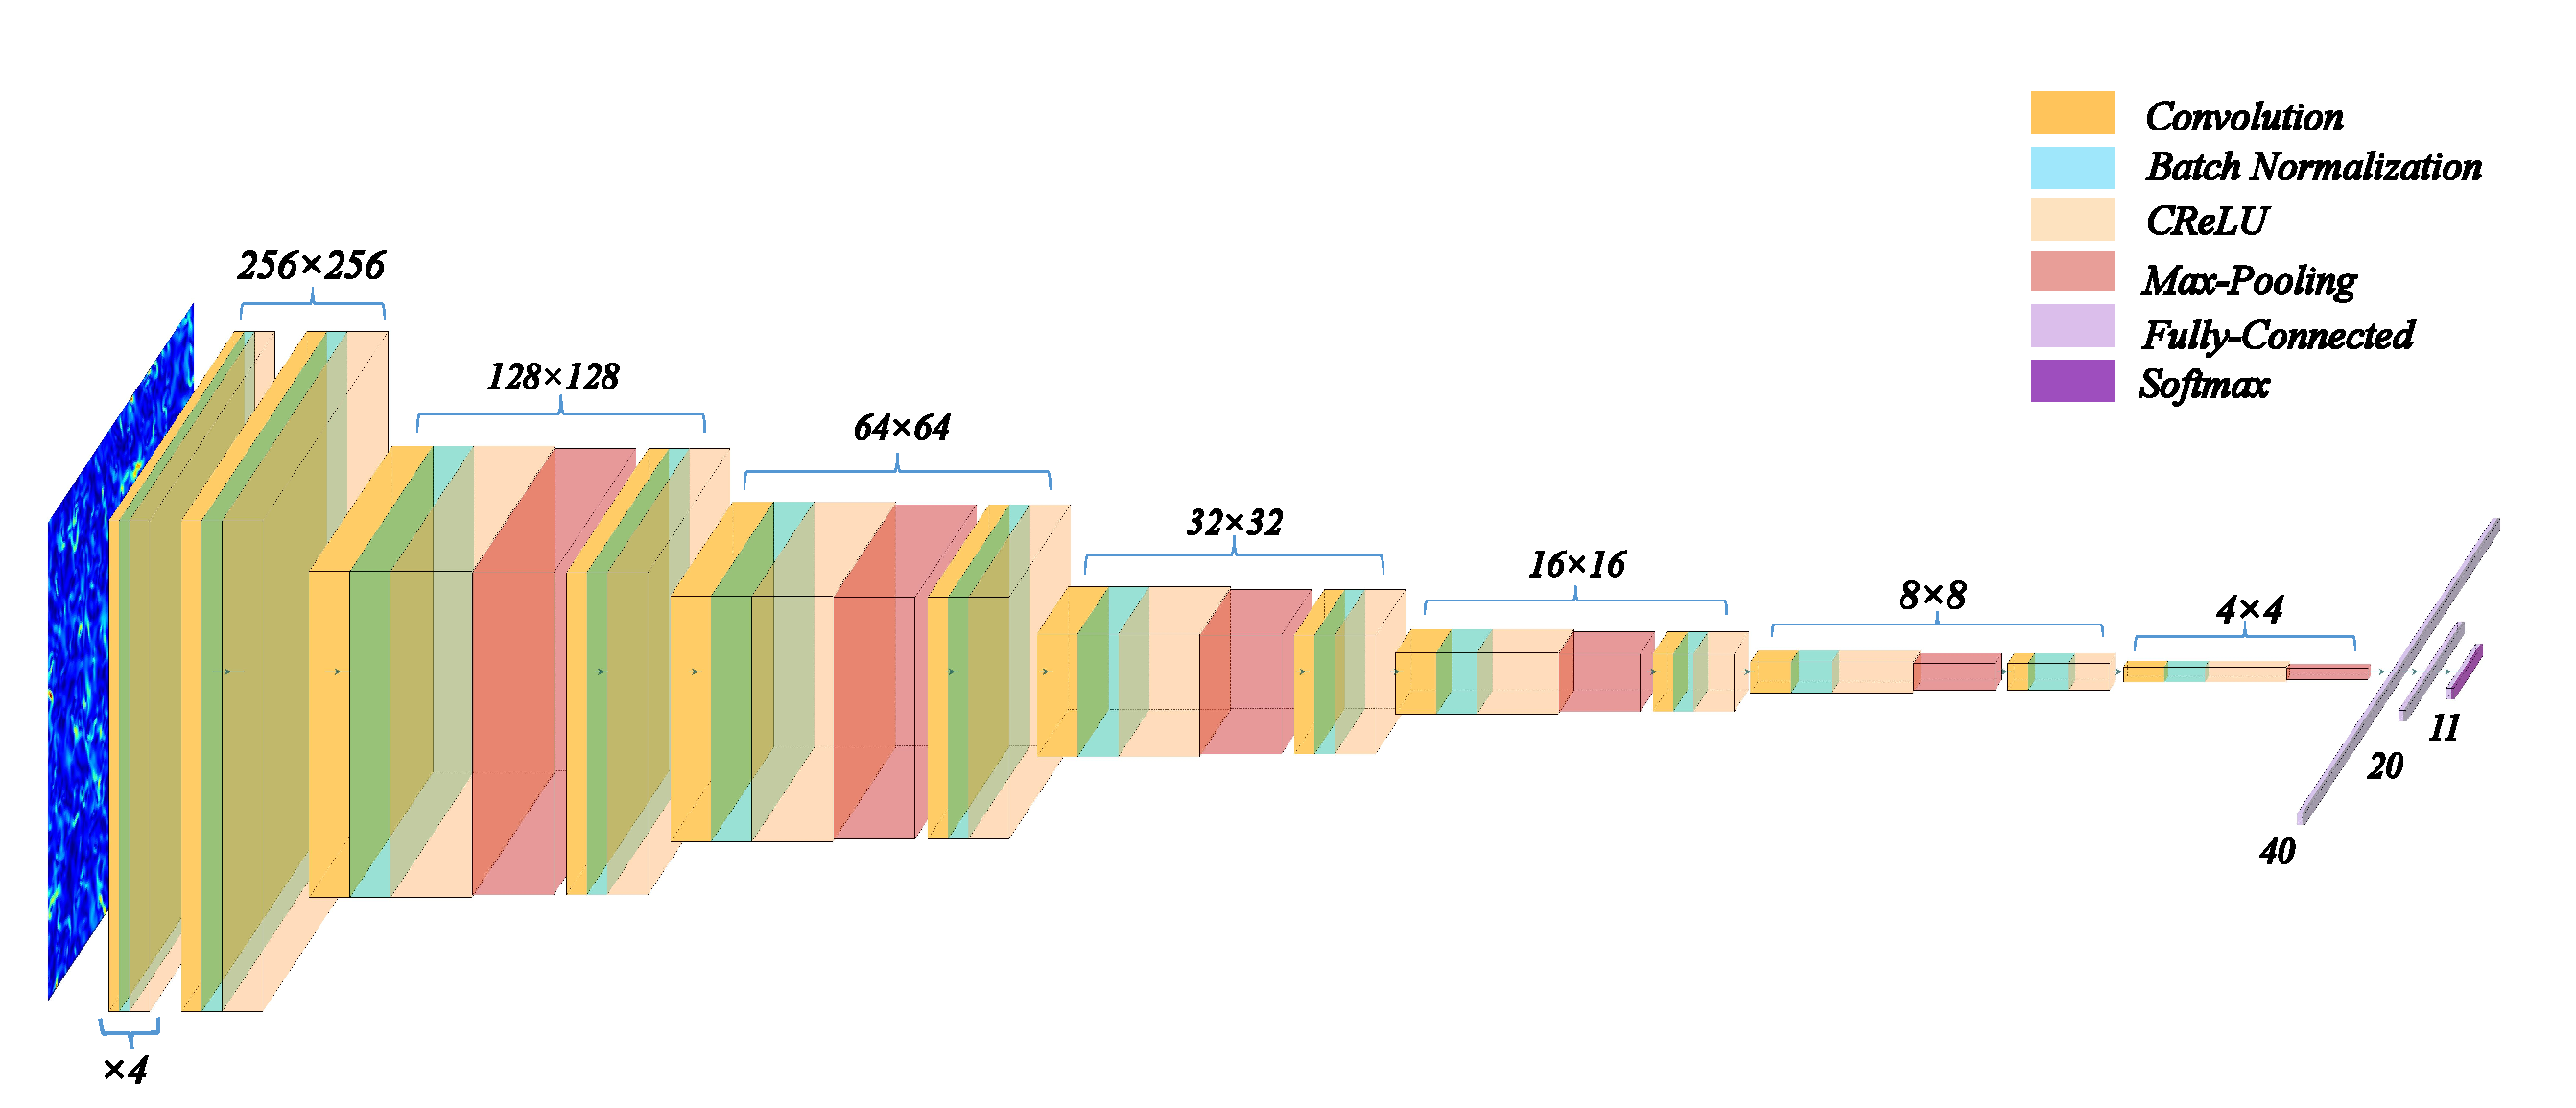
\includegraphics[width=\linewidth , height=0.35\textheight]{figs/arch_vis.pdf}
	\end{center}
	\caption[
			نمایش تجسمی معماری شبکه نهایی و تغییر ابعاد تصویر در طول پیش رفتن در لایه‌های مختلف. طول و عرض حاصل از هر لایه در بالای آن نوشته شده است. عمق هر لایه نیز به ابرپارامترهای آن لایه برمی‌گردد. ورودی شبکه نقشه‌های با ابعاد 
	۲۵۶$\times$۲۵۶
	هستند و خروجی شبکه یا آرایه یک بعدی با ۱۱ عنصر است که هر کدام از عناصر احتمال تعلق داده ورودی به ۱۱ کلاس مختلف از تنش ریسمان را نشان می‌دهد.  
	]{
		نمایش تجسمی معماری شبکه نهایی و تغییر ابعاد تصویر در طول پیش رفتن در لایه‌های مختلف. طول و عرض حاصل از هر لایه در بالای آن نوشته شده است. عمق هر لایه نیز به ابرپارامترهای آن لایه برمی‌گردد. ورودی شبکه نقشه‌های با ابعاد 
		۲۵۶$\times$۲۵۶
		هستند و خروجی شبکه یا آرایه یک بعدی با ۱۱ عنصر است که هر کدام از عناصر احتمال تعلق داده ورودی به ۱۱ کلاس مختلف از تنش ریسمان را نشان می‌دهد.    
		\footnotemark.}
	\label{fig:arch_vis}
\end{figure} 
\footnotetext{برای ساخت این شکل از کد 
	\lr{PlotNeuralNet}
	در لتک استفاده کرده‌ام: \\
	\url{https://github.com/HarisIqbal88/PlotNeuralNet}}
%-------------------------------------------------------------------------
در نتیجه‌ی آزمودن شبکه‌های مختلف به نتایجی دست پیدا کردیم که برای رسیدن به مدل بهینه مفید بودند:
\begin{itemize}
	\item 
	وجود گام یا 
	\lr{stride}
	بزرگتر از ۱ در لایه پیچشی مفیدتر از این است که همه سهم گام‌ها را به لایه ادغام بدهیم. از آن‌جایی که گام بزرگتر از ۱ موجب کاهش بعد تصویر ورودی می‌شود در تعداد گام‌های کل شبکه محدودیت وجود دارد و نمی‌توانیم به همه لایه‌ها سهمی از گام بدهیم.   
	\item
	بهتر است از ادغام بیشینه در شبکه استفاده کنیم. تجربه نشان داده است که ادغام بیشینه بهتر از ادغام میانگین به لبه‌یابی در تصویر کمک می‌کند. 
	\item
	 فیلتر با ابعاد ۵$\times$۵ انتخاب بهینه‌ای است. فیلتر کوچکتر (۳) شبکه را بیش از حد ساده می‌کند و فیلتر بزرگتر (۷) هزینه محاسباتی بسیار بالایی دارد که به استفاده از آن نمی‌ارزد. 
\end{itemize}

پس از طی مراحل طاقت فرسا و زمان‌بر سعی و خطا :) ، به معماری مناسبی برای شبکه عصبی دست یافتیم. 
طبق این دو معیار شبکه‌های مختلف را با هم مقایسه کردیم و در پایان به معماری توصیف شده در جدول 
\ref{Table:arch}
رسیدیم. در شبکه منتخب، در مجموع ۱۶ لایه پیچشی وجود دارد که در ادامه‌ی هر کدام یک لایه ‌BN و لایه تابع فعال‌سازی وجود دارد. علت اینکه تابع فعال‌سازی را به عنوان یک لایه جدا قرار داده‌ایم در حالی که می‌توانست درون لایه پیچشی قرار بگیرد، این است که فعال‌سازی باید بعد از مرحل بهنجارش در BN صورت بگیرد. لایه‌های شبکه در دو بلوک قرار دارند. بلوک اول شامل یک لایه پیچشی( البته به همراه مخلفات!) است که ۴ بار تکرار می‌شود. در این بلوک گام پیچش ۱ است و لایه ادغام نیز وجود ندارد. بنابراین این بلوک منجر به هیچ تغییری در طول و عرض تصویر ورودی نمی‌شود. عمق هر لایه پیچشی  با توجه به تعداد فیلترها مشخص می‌شود و لایه CReLU عمق ورودی را دو برابر می‌کند ولی لایه BN تغییری در عمق ورودی ایجاد نمی‌کند. بلوک دوم شامل ۶ بار تکرار یک الگوست که شامل دو لایه پیچشی است. قسمت اول همانند لایه‌های بلوک اول است اما قسمت دوم شامل لایه پیچشی با گام ۲ است. در انتهای این بلوک یک لایه ادغام با گام ۲ و اندازه ادغام ۲ وجود دارد. لذا بار کاهش ابعاد در این شبکه بر دوش قسمت دوم بلوک دوم است. تصویر پس از گذر از این دو بلوک از لایه‌های پیچشی باید وارد لایه کاملا همبند شود. از ان جایی که خروجی لایه های پیچشی ۲بعدی است و ورودی لایه کاملا همبند باید ۱بعدی است از لایه FLatten  برای تبدیل آرایه دوبعدی به یک بعدی استفاده می‌کنیم. در انتها ۳ لایه کاملا همبند وجود دارد که خروجی لایه آخر یک آرایه یک بعدی با ۱۱ عنصر است، همانگونه که انتظار داشته‌ایم. تابع فعال‌سازی لایه آخر Softmax است که در مسائل طبقه‌بندی چند کلاسه به صورت گسترده به عنوان فعالسازی لایه آخر استفاده می‌شود. شکل
\ref{fig:arch_vis}
چگونگی کاهش ابعاد تصویر ورودی را در طول شبکه نشان می‌دهد.        



%-------------------------------------------------------------------------
\subsection{فرآیند یادگیری}
%----------------------------
\begin{figure}[h!]
	\centering
	\begin{subfigure}{0.5\textwidth}
		\centering
		\includegraphics[scale=0.5]{figs/1_acc_noiseless.png}
		\caption{ تغییرات دقت پیش‌بینی‌ ماشین در طول گام‌های یادگیری.  }
		%		\label{fig:sub1}
	\end{subfigure}%
	\begin{subfigure}{0.5\textwidth}
		\centering
		\includegraphics[scale=0.5]{figs/1_loss_noiseless.jpg}
		\caption{ تغییرات مقدار تابع هزینه در طول گام‌های یادگیری. }
		%		\label{fig:sub2}
	\end{subfigure}
	
	\caption{  تحولات دقت  و مقدار هزینه در طول گام‌های آموزش ماشین 
		برای شبیه‌سازی Healpix ایده‌آل و بدون نوفه. در شکل سمت راست، دقت روی داده‌های آموزش با رنگ سبز و داده‌های آزمون با رنگ قرمز مشخص شده است. مطابق شکل دقت روی داده‌های آزمون گرچه کمی کمتر از  دقت روی داده‌های آموزش است ولی این مقدار تفاوت طبیعی و قابل انتظار است و به معنای برازش بیش از حد نیست. شکل سمت چپ نشان‌دهنده مقادیر تابع هزینه است. مقدار اولیه هزینه، بستگی به انتخاب تابع هزینه دارد. هرچه شدت نوفه بیشتر شود، تابع هزینه به مقادیر بزرگ‌تری همگرا می‌شود.}
	\label{fig:epoch}
\end{figure}
%----------------------------
معماری نهایی مدلی با حدود ۹۰۰۰۰ پارامتر آزاد می‌سازد که آموزش ماشین به معنی پیدا کردن بهترین برازش برای همه این پارامتر‌ها است. این فرآیند برای ورودی‌های با طول و عرض ۲۵۶ پیکسل، به حدودا ۵ ساعت زمان برای اجرا شدن روی یک پردازنده گرافیکی
\LTRfootnote{Graphics processing unit}
\lr{Tesla K80 GPU}
نیاز دارد.
تابع هزینه‌ای که برای آموزش ماشین استفاده کرده‌ایم، تابع Hubber loss معادله
\ref{huber_loss}
است. گرچه نتایج تابع هزینه Cross Entropy معادله
\ref{CE_loss}
 و Logloss 
%\ref{CE_loss}
 نیز امیدبخش بوده است. از AdamOptimizer نیز برای بهینه‌سازی استفاده شده است. مقدار نرخ یادگیری را در ابتدای فرآیند آموزش $0.001$ قرار دادیم و در حین یادگیری هر زمانی که مقدار هزینه در چند مرحله از یادگیری ثابت ماند و پیشرفت زیادی نکرد به مرور کاهش دادیم. نرخ یادگیری تا مقدار $0.000005$ نیز کاهش پیدا می‌کند.
 در طول فرآیند آموزش همواره باید خطر برازش بیش از حد را مدّ نظر قرار داد. برای اینکه مطمئن باشیم برازش بیش از اندازه رخ نداده است باید همواره در بازه‌های زمانی کوتاه دقت روی داده‌های آموزش و روی داده‌های آزمون را مقایسه کنیم. اگر تفاوت معنی‌دار (به طور مثال حداکثر بیش از ۱۰ درصد تفاوت) وجود داشت به این معنی است که مدل در حال برازش بیش از حد شدن است. ترسیم ماتریس درهم‌ریختگی برای داده‌های آموزش و آزمون هم راه دقیقی برای سنجش برازش ماشین است. در مدلی که به برازش بیش از حد دچار نباشد نباید تفاوت فاحشی بین این دو ماتریس وجود داشته باشد. 
  در شکل 
\ref{fig:epoch} 
تحول مقدار هزینه در طول زمان یادگیری و هم‌چنین تغییرات دقت ماشین برای داده‌های Healpix بدون نوفه و کاملا ایده‌آل نشان داده ‌شده است. فرآیند ساخت مدل و آموزش آن توسط بسته نرم‌افزاری تنسورفلو
\LTRfootnote{Tensorflow :\url{www.tensorflow.org}}
\cite{abadi2016tensorflow}
و در محیط پایتون انجام شده است. برای سهولت بیشتر در کار با تنسورفلو، از بسته نرم‌افزاری 
Ngene 
\LTRfootnote{\url{github.com/vafaei-ar/Ngene.git}}
استفاده شده است. کدهای مربوط به این تحقیق در گیت‌هاب
\LTRfootnote{github}
 به آدرس
\url{github.com/M-Torki/DeePlanck.git }
در دسترس است.
  
  
  
  \section{نتایج آموزش ماشین روی داده‌های شبیه‌سازی }
  \label{sec:results}
  
  مطابق روشی که در این فصل شرح داده شد و پس از آن که به یک معماری بهینه برای شبکه پیچشی رسیدیم، شبکه را برای انواع شبیه‌سازی‌هایی که در این تحقیق مدّ نظر است به صورت جداگانه آموزش دادیم. پس از اجرای فرآیند آموزش، متناظر با هر دسته شبیه‌سازی به یک مدل نهایی دست پیدا کردیم. برای گزارش دقت هر مدل و حدی از تنش ریسمان که ماشین قادر به دیدن و تشخیص آن است از دو معیار مقدار پی و ماتریس درهم‌ریختگی استفاده کرده‌ایم که متناظر با هر کدام از این معیارها ۲ کمیت معرفی می‌کنیم:
  \begin{description}
  	\item
  	کمینه قابل اندازه‌گیری یا $G\mu_{mes}$:\\
  	این کمیت برای ماتریس درهم‌ریختگی تنشی است که ماشین با $\%$۹۵ دقت ($\sigma$2) توانایی تشخیص و اندازه‌گیری آن را دارد. این مقدار در ماتریس معادل کلاسی است که آرایه روی قطر متناظر با آن $\%$۹۵ باشد. از آن‌جایی که مقادیر روی قطر گاهی کمی کمتر یا بیشتر از $\%$۹۵ هستند برای به دست آوردن حدود تنشی که دقت اندازه‌گیری آن دقیقا مساوی ۹۵ شود مقادیر روی قطر ماتریس را درون‌یابی می‌کنیم. در اینجا ما برای ساده‌سازی فرض می‌کنیم که رفتار تابع خطی است.
  	علاوه بر ماتریس درهم‌ریختگی، حد کمینه قابل اندازه‌گیری را می‌توان با اطلاعات مقادیر پی برای کلاس‌های مختلف به دست آورد. طبق تعریف ما مقدار تنشی که قابل اندازه گیری است لزوما باید از تمام کلاس‌های دیگر قابل تمایز باشد. یعنی مقدار پی بین توزیع مربوط به این مقدار کمینه و توزیع تمام کلاس‌های دیگر کمتر از $0.05$ باشد که معادل دقت $\sigma$2 است. همانند روش به دست آوردین کمینه قابل اندازه‌گیری با ماتریس، برای محاسبه مقدار دقیق این حد با مقدار پی باید درون‌یابی انجام دهیم.     
  	\item
  	کمینه قابل آشکارسازی یا $G\mu_{det}$:\\
  	آشکارسازی به معنای تشخیص دادن نقشه‌های ریسمان‌دار از نقشه‌ی پوچ و بدون ریسمان است. مشابه حد قابل اندازه‌گیری، این حد را هم از دو منظر ماتریس درهم‌ریختگی و مقدار پی به دست می‌آوریم. از منظر ماتریس درهم‌ریختگی، حد قابل آشکارسازی مقدار تنشی است که کمتر از $\%$۵ نمونه‌های مربوط به آن با کلاس پوچ یا صفر توسط ماشین اشتباه گرفته شده باشد. به عبارتی مقادیر ستون اول در ماتریس برای ما مهم است. اولین کلاسی که آرایه مربوط به آن در ستون اول کوچکتر یا مساوی $0.05$ باشد حد قابل آشکارسازی را مشخص می‌کند. برخلاف قبل که گفتیم مقادیر را درون‌یابی کرده‌ایم، برای این حد به گزارش برچسب کلاس مربوطه اکتفا می‌کنیم. حد قابل آشکارسازی توسط مقادیر پی نیز قابل محاسبه است. برای این کار توزیع پیش‌بینی‌های مربوط به هر کلاس را با توزیع پیش‌بینی‌های کلاس صفر یا پوچ مقایسه می کنیم و مقدار پی مربوطه را به دست می‌آوریم. آستانه مورد نظر در این مورد هم دقت $\sigma$2 یا همان مقدار پی $0.05$ است.   	    
  \end{description}
  در بخش بعدی حدود قابل اندازه‌گیری و حدود قابل آشکارسازی را برای ۷ حالت شبیه‌سازی مختلفی که بررسی کرده‌ایم بیان خواهیم کرد. ماتریس در‌هم‌ریختگی و نمودار‌های مربوط به مقدار پی نیز برای همه شبیه‌سازی‌ها آورده شده است.  
%  \newpage  
  %-------------------------------------------------------------------------
  \subsection{حدود قابل اندازه‌گیری و قابل آشکارسازی به دست آمده}
  \label{subsec:upper_bounds}
  
\subsubsection{آزمایش شبه نسل چهارم تابش زمینه-نوع دوم}
نتایج به دست آمده برای آزمایش شبه نوع دوم نسل چهار، با\\
$N_{side} = 4096$ \\
$SNR=20$\\
$FWHM = 0.9'$
به شرح زیر است:\\
قدرت اندازه‌گیری مدل با معیار ماتریس در‌هم‌ریختگی مقدار 
$G\mu \geq 1.9\times 10^{-7}$
و با معیار مقدار پی 
$G\mu \geq 1.7\times 10^{-7}$
است. هم‌چنین قدرت آشکارسازی مدل با معیار ماتریس در‌هم‌ریختگی مقدار
$G\mu \geq 8.9\times 10^{-8}$
و با معیار مقدار پی 
$G\mu \geq 2.6\times 10^{-8}$
است. اطلاعات مربوط به مقادیر پی در شکل
\ref{fig:s4ii_pv}
و اطلاعات ماتریس درهم‌ریختگی در شکل
\ref{fig:s4ii_cm}
 آمده است.
  	
  	\begin{figure}
  		\centering
  		\begin{subfigure}{0.5\textwidth}
  			\centering
  			\includegraphics[scale=0.5]{figs/pv_m_s4ii.png}
  			\caption{   کمینه تنش قابل اندازه‌گیری برای آزمایش
  				\\	 شبه نوع دوم نسل چهار
  				بر اساس آمار \lr{P\;value}}
  			%		\label{fig:sub1}
  		\end{subfigure}%
  		\begin{subfigure}{0.5\textwidth}
  			\centering
  			\includegraphics[scale=0.5]{figs/pv_d_s4ii.png}
  			\caption{  کمینه تنش قابل آشکارسازی برای آزمایش 
  				\\ شبه نوع دوم نسل چهار
  				بر اساس آمار \lr{P\;value} }
  			%		\label{fig:sub2}
  		\end{subfigure}
  		
  		\caption{حدود قابل اندازه‌گیری و آشکارسازی برای آزمایش شبه نوع دوم نسل چهارم تابش زمینه
  			به وسیله درون‌یابی مقادیر پی.}
  		\label{fig:s4ii_pv}
  	\end{figure}
  	%------------------------
  	\begin{figure}
  		\centering
  		\begin{subfigure}{\textwidth}
  			\centering
  			\includegraphics[scale=0.7]{figs/cm_s4ii.png}
  			\caption{  ماتریس درهم‌ریختگی برای  
  			آزمایش شبه نوع دوم نسل چهار}
  			%		\label{fig:sub1}
  		\end{subfigure}%
  		
  		\begin{subfigure}{0.5\linewidth}
  			\centering
  			\includegraphics[width=\textwidth , height=0.22\textheight]{figs/cm_m_s4ii.png}
  			\caption{  کمینه تنش قابل اندازه‌گیری توسط ماشین برای آزمایش شبه نوع دوم نسل چهار}
  			%		\label{fig:sub2}
  		\end{subfigure}
  		
  		\caption{ماتریس در هم ریختگی برای دسته‌بندی داده‌های آزمایش شبه نوع دوم نسل چهارم تابش زمینه
  			و به دست آوردن حد کمینه قابل اندازه‌گیری توسط ماشین از روی این ماتریس به وسیله درون‌یابی عناصر قطر.}
  		\label{fig:s4ii_cm}
  	\end{figure}
  	
  	
  	
  	%-------------------------------------------------------------------------
  	\subsubsection{آزمایش شبه نسل چهارم تابش زمینه-نوع اول} 
  	نتایج به دست آمده برای آزمایش شبه نوع اول نسل چهار، با\\
  	$N_{side} = 4096$ \\
  	$SNR=15$\\
   	$FWHM = 0.9'$
  	به شرح زیر است:\\
  	قدرت اندازه‌گیری مدل با معیار ماتریس در‌هم‌ریختگی مقدار 
  	$G\mu \geq 1.9\times 10^{-7}$
  	و با معیار مقدار پی 
  	$G\mu \geq 1.6\times 10^{-7}$
  	است. هم‌چنین قدرت آشکارسازی مدل با معیار ماتریس در‌هم‌ریختگی مقدار
  	$G\mu \geq 1.9\times 10^{-7}$
  	و با معیار مقدار پی 
  	$G\mu \geq 1.3\times 10^{-7}$
  	است. اطلاعات مربوط به مقادیر پی در شکل
  	\ref{fig:s4i_pv}
  	و اطلاعات ماتریس درهم‌ریختگی در شکل
  	\ref{fig:s4i_cm}
  	آمده است.
  	
  	
  	
  	\begin{figure}
  		\centering
  		\begin{subfigure}{0.5\textwidth}
  			\centering
  			\includegraphics[scale=0.5]{figs/pv_m_s4i.png}
  			\caption{   کمینه تنش قابل اندازه‌گیری برای آزمایش 
  				\\	 شبه نوع اول نسل چهار
  				بر اساس آمار \lr{P\;value}}
  			%		\label{fig:sub1}
  		\end{subfigure}%
  		\begin{subfigure}{0.5\textwidth}
  			\centering
  			\includegraphics[scale=0.5]{figs/pv_d_s4i.png}
  			\caption{  کمینه تنش قابل آشکارسازی برای آزمایش 
  				\\  شبه نوع اول نسل چهار
  				بر اساس آمار \lr{P\;value} }
  			%		\label{fig:sub2}
  		\end{subfigure}
  		
  		\caption{حدود قابل اندازه‌گیری و آشکارسازی برای آزمایش 
شبه نوع اول نسل چهارم تابش زمینه به وسیله درون‌یابی مقادیر پی.}
  		\label{fig:s4i_pv}
  	\end{figure}
  	%------------------------
  	\begin{figure}
  		\centering
  		\begin{subfigure}{\textwidth}
  			\centering
  			\includegraphics[scale=0.7]{figs/cm_s4i.png}
  			\caption{  ماتریس درهم‌ریختگی برای آزمایش 
  				شبه نوع اول نسل چهار }
  			%		\label{fig:sub1}
  		\end{subfigure}%
  		
  		\begin{subfigure}{0.5\linewidth}
  			\centering
  			\includegraphics[width=\textwidth , height=0.22\textheight]{figs/cm_m_s4i.png}
  			\caption{  کمینه تنش قابل اندازه‌گیری توسط ماشین برای آزمایش 
  				شبه نوع اول نسل چهار }
  			%		\label{fig:sub2}
  		\end{subfigure}
  		
  		\caption{ماتریس در هم ریختگی برای دسته‌بندی داده‌های آزمایش
شبه نوع اول نسل چهارم تابش زمینه و به دست آوردن حد کمینه قابل اندازه‌گیری توسط ماشین از روی این ماتریس به وسیله درون‌یابی عناصر قطر.}
  		\label{fig:s4i_cm}
  	\end{figure}
  	
  	
  	
  	
  	%-------------------------------------------------------------------------
  	
\subsubsection{آزمایش‌ شبه تلسکوپ کیهان‌شناسی آتاکاما}
  	نتایج به دست آمده برای آزمایش شبه تلسکوپ کیهان‌شناسی آتاکاما ، با\\
  	$N_{side} = 4096$ \\
  	$SNR=10$\\
  	$FWHM = 0.9'$
  	به شرح زیر است:\\
  	قدرت اندازه‌گیری مدل با معیار ماتریس در‌هم‌ریختگی مقدار 
  	$G\mu \geq 4.1\times 10^{-7}$
  	و با معیار مقدار پی 
  	$G\mu \geq 3.5\times 10^{-7}$
  	است. هم‌چنین قدرت آشکارسازی مدل با معیار ماتریس در‌هم‌ریختگی مقدار
  	$G\mu \geq 1.9\times 10^{-7}$
  	و با معیار مقدار پی 
  	$G\mu \geq 2.4\times 10^{-7}$
  	است.
  	اطلاعات مربوط به مقادیر پی در شکل
  	\ref{fig:act_pv}
  	و اطلاعات ماتریس درهم‌ریختگی در شکل
  	\ref{fig:act_cm}
  	آمده است.
  	
  	\begin{figure}
  		\centering
  		\begin{subfigure}{0.5\textwidth}
  			\centering
  			\includegraphics[scale=0.5]{figs/pv_m_act.png}
  			\caption{   کمینه تنش قابل اندازه‌گیری برای آزمایش  
  				\\	شبه تلسکوپ آتاکاما
  				بر اساس آمار \lr{P\;value} }
  			%		\label{fig:sub1}
  		\end{subfigure}%
  		\begin{subfigure}{0.5\textwidth}
  			\centering
  			\includegraphics[scale=0.5]{figs/pv_d_act.png}
  			\caption{  کمینه تنش قابل آشکارسازی برای آزمایش 
  				\\ شبه تلسکوپ آتاکاما
  				بر اساس آمار 
  				\lr{P\;value}. }
  			%		\label{fig:sub2}
  		\end{subfigure}
  		
  		\caption{حدود قابل اندازه‌گیری و آشکارسازی برای آزمایش 
شبه تلسکوپ آتاکاما به وسیله درون‌یابی مقادیر پی.}
  		\label{fig:act_pv}
  	\end{figure}
  	%------------------------
  	\begin{figure}
  		\centering
  		\begin{subfigure}{\textwidth}
  			\centering
  			\includegraphics[scale=0.7]{figs/cm_act.png}
  			\caption{  ماتریس درهم‌ریختگی برای آزمایش شبه تلسکوپ آتاکاما }
  			%		\label{fig:sub1}
  		\end{subfigure}%
  		
  		\begin{subfigure}{0.5\linewidth}
  			\centering
  			\includegraphics[width=\textwidth , height=0.22\textheight]{figs/cm_m_act.png}
  			\caption{  کمینه تنش قابل اندازه‌گیری توسط ماشین برای آزمایش شبه تلسکوپ آتاکاما }
  			%		\label{fig:sub2}
  		\end{subfigure}
  		
  		\caption{ماتریس در هم ریختگی برای دسته‌بندی داده‌های آزمایش شبه تلسکوپ آتاکاما
  			و به دست آوردن حد کمینه قابل اندازه‌گیری توسط ماشین از روی این ماتریس به وسیله درون‌یابی عناصر قطر.}
  		\label{fig:act_cm}
  	\end{figure}
  	
  	
  	%-------------------------------------------------------------------------
  	
  \subsubsection{  	شبیه‌سازی  \lr{FFP10}}
   	\begin{itemize}
   		\item \textbf{حالت ایده‌آل بدون نوفه} \\
   		   	نتایج به دست آمده برای شبیه‌سازی‌های بدون نوفه
   		   	\lr{FFP10}
   		   	با\\
   		$N_{side} = 2048$ \\
   		$FWHM = 5'$
   		  به شرح زیر است:\\
   		قدرت اندازه‌گیری مدل با معیار ماتریس در‌هم‌ریختگی مقدار 
   		$G\mu \geq 8.6\times 10^{-8}$
   		و با معیار مقدار پی 
   		$G\mu \geq 8.1\times 10^{-8}$
   		است. هم‌چنین قدرت آشکارسازی مدل با معیار ماتریس در‌هم‌ریختگی مقدار
   		$G\mu \geq 4.1\times 10^{-8}$
   		و با معیار مقدار پی 
   		$G\mu \geq 3.2\times 10^{-8}$
   		است.
   		اطلاعات مربوط به مقادیر پی در شکل
   		\ref{fig:ffp_pv}
   		و اطلاعات ماتریس درهم‌ریختگی در شکل
   		\ref{fig:ffp_cm}
   		آمده است.
   		
		\item \textbf{با نوفه رصدی} \\
		نتایج به دست آمده برای شبیه‌سازی‌های \lr{FFP10}
		با\\
		 $N_{side} = 2048$ \\
 		 $SNR=10$\\
		 $FWHM = 5'$\\
		 به شرح زیر است:\\
		 قدرت اندازه‌گیری مدل با معیار ماتریس در‌هم‌ریختگی مقدار 
		 $G\mu \geq 6.8\times 10^{-7}$
		 و با معیار مقدار پی 
		 $G\mu \geq 3.6\times 10^{-7}$
		 است. هم‌چنین قدرت آشکارسازی مدل با معیار ماتریس در‌هم‌ریختگی مقدار
		 $G\mu \geq 4.1\times 10^{-7}$
		 و با معیار مقدار پی 
		 $G\mu \geq 1.4\times 10^{-7}$
		 است.
		 اطلاعات مربوط به مقادیر پی در شکل
		 \ref{fig:nffp_pv}
		 و اطلاعات ماتریس درهم‌ریختگی در شکل
		 \ref{fig:nffp_cm}
		 آمده است.
		
		 
   	\end{itemize}

  	
  	\begin{figure}
  		\centering
  		\begin{subfigure}{0.5\textwidth}
  			\centering
  			\includegraphics[scale=0.5]{figs/pv_m_ffp.png}
  			\caption{   کمینه تنش قابل اندازه‌گیری برای شبیه‌سازی 
  				\\	\lr{FFP10} 
  				بدون نوفه بر اساس آمار 
  				\lr{P\;value}. }
  			%		\label{fig:sub1}
  		\end{subfigure}%
  		\begin{subfigure}{0.5\textwidth}
  			\centering
  			\includegraphics[scale=0.5]{figs/pv_d_ffp.png}
  			\caption{  کمینه تنش قابل آشکارسازی برای شبیه‌سازی 
  				\\	\lr{FFP10} 
  				بدون نوفه بر اساس آمار 
  				\lr{P\;value}. }
  			%		\label{fig:sub2}
  		\end{subfigure}
  		
  		\caption{حدود قابل اندازه‌گیری و آشکارسازی برای شبیه‌سازی 
  					\lr{FFP10} 
  			بدون نوفه به وسیله درون‌یابی مقادیر پی}
  		\label{fig:ffp_pv}
  	\end{figure}
  	%------------------------
  	\begin{figure}
  		\centering
  		\begin{subfigure}{0.5\textwidth}
  			\centering
  			\includegraphics[scale=0.5]{figs/pv_m_nffp.png}
  			\caption{   کمینه تنش قابل اندازه‌گیری برای شبیه‌سازی 
  				\\	\lr{FFP10} 
  				بر اساس آمار 
  				\lr{P\;value} }
  			%		\label{fig:sub1}
  		\end{subfigure}%
  		\begin{subfigure}{0.5\textwidth}
  			\centering
  			\includegraphics[scale=0.5]{figs/pv_d_nffp.png}
  			\caption{  کمینه تنش قابل آشکارسازی برای شبیه‌سازی 
  				\\	\lr{FFP10} 
  				بر اساس آمار 
  				\lr{P\;value} }
  			%		\label{fig:sub2}
  		\end{subfigure}
  		
  		\caption{حدود قابل اندازه‌گیری و آشکارسازی برای شبیه‌سازی 
  				\lr{FFP10} 
  			به وسیله درون‌یابی مقادیر پی.}
  		\label{fig:nffp_pv}
  	\end{figure}
  	%------------------------
  	\begin{figure}
  		\centering
  		\begin{subfigure}{\textwidth}
  			\centering
  			\includegraphics[scale=0.7]{figs/cm_ffp.png}
  			\caption{  ماتریس درهم‌ریختگی برای شبیه‌سازی 
  					\lr{FFP10} 
  				بدون نوفه }
  			%		\label{fig:sub1}
  		\end{subfigure}%
  		
  		\begin{subfigure}{0.5\linewidth}
  			\centering
  			\includegraphics[width=\textwidth , height=0.22\textheight]{figs/cm_m_ffp.png}
  			\caption{  کمینه تنش قابل اندازه‌گیری توسط ماشین برای شبیه‌سازی 
  					\lr{FFP10} 
  				بدون نوفه }
  			%		\label{fig:sub2}
  		\end{subfigure}
  		
  		\caption{ماتریس در هم ریختگی برای دسته‌بندی داده‌های شبیه‌سازی
  			  		\lr{FFP10}  
  			بدون نوفه و به دست آوردن حد کمینه قابل اندازه‌گیری توسط ماشین از روی این ماتریس به وسیله درون‌یابی عناصر قطر.}
  		\label{fig:ffp_cm}
  	\end{figure}
  	%------------------------
  	\begin{figure}
  		\centering
  		\begin{subfigure}{\textwidth}
  			\centering
  			\includegraphics[scale=0.7]{figs/cm_nffp.png}
  			\caption{  ماتریس درهم‌ریختگی برای شبیه‌سازی 
  				  	\lr{FFP10}  
  			}
  			%		\label{fig:sub1}
  		\end{subfigure}%
  		
  		\begin{subfigure}{0.5\linewidth}
  			\centering
  			\includegraphics[width=\textwidth , height=0.22\textheight]{figs/cm_m_nffp.png}
  			\caption{  کمینه تنش قابل اندازه‌گیری توسط ماشین برای شبیه‌سازی 
  					\lr{FFP10} 
  			}
  			%		\label{fig:sub2}
  		\end{subfigure}
  		
  		\caption{ماتریس در هم ریختگی برای دسته‌بندی داده‌های شبیه‌سازی
  					\lr{FFP10} 
  			و به دست آوردن حد کمینه قابل اندازه‌گیری توسط ماشین از روی این ماتریس به وسیله درون‌یابی عناصر قطر.}
  		\label{fig:nffp_cm}
  	\end{figure}
  	
  	%-------------------------------------------------------------------------
  	
    	
  \subsubsection{  	شبیه‌سازی End-to-End }
  \begin{itemize}
  	\item \textbf{حالت ایده‌آل بدون نوفه} \\
  	نتایج به دست آمده برای شبیه‌سازی‌های بدون نوفه
  	\lr{E2E}
  	با\\
  	$N_{side} = 2048$ \\
  	$FWHM = 5'$
  	به شرح زیر است:\\
  	قدرت اندازه‌گیری مدل با معیار ماتریس در‌هم‌ریختگی مقدار 
  	$G\mu \geq 7.2\times 10^{-7}$
  	و با معیار مقدار پی 
  	$G\mu \geq 1.9\times 10^{-7}$
  	است. هم‌چنین قدرت آشکارسازی مدل با معیار ماتریس در‌هم‌ریختگی مقدار
  	$G\mu \geq 4.1\times 10^{-7}$
  	و با معیار مقدار پی 
  	$G\mu \geq 1.4\times 10^{-7}$
  	است.
  	اطلاعات مربوط به مقادیر پی در شکل
  	\ref{fig:e2eless_pv}
  	و اطلاعات ماتریس درهم‌ریختگی در شکل
  	\ref{fig:E2Eless_cm}
  	آمده است.
  	
  	\item \textbf{با نوفه رصدی} \\
  	نتایج به دست آمده برای شبیه‌سازی‌های \lr{E2E}
  	با\\
  	$N_{side} = 2048$ \\
  	$SNR=8$\\
  	$FWHM = 5'$\\
  	به شرح زیر است:\\
  	قدرت اندازه‌گیری مدل با معیار ماتریس در‌هم‌ریختگی مقدار 
  	$G\mu \geq 8.8\times 10^{-7}$
  	و با معیار مقدار پی 
  	$G\mu \geq 4.9\times 10^{-7}$
  	است. هم‌چنین قدرت آشکارسازی مدل با معیار ماتریس در‌هم‌ریختگی مقدار
  	$G\mu \geq 8.8\times 10^{-7}$
  	و با معیار مقدار پی 
  	$G\mu \geq 3.7\times 10^{-7}$
  	است.
  	اطلاعات مربوط به مقادیر پی در شکل
  	\ref{fig:nsyE2E_pv}
  	و اطلاعات ماتریس درهم‌ریختگی در شکل
  	\ref{fig:nsye2e_cm}
  	آمده است.
  	
  	
  \end{itemize}
  	
  	\begin{figure}
  		\centering
  		\begin{subfigure}{0.5\textwidth}
  			\centering
  			\includegraphics[scale=0.5]{figs/pv_m_e2eless.png}
  			\caption{   کمینه تنش قابل اندازه‌گیری برای شبیه‌سازی 
  				\\			\lr{E2E}
  				بدون نوفه بر اساس آمار
  				\lr{P\;value} }
  			%		\label{fig:sub1}
  		\end{subfigure}%
  		\begin{subfigure}{0.5\textwidth}
  			\centering
  			\includegraphics[scale=0.5]{figs/pv_d_e2eless.png}
  			\caption{  کمینه تنش قابل آشکارسازی برای شبیه‌سازی 
  				\\ 		\lr{E2E}
  				بدون نوفه بر اساس آمار
  				\lr{P\;value}	
  			}
  			%		\label{fig:sub2}
  		\end{subfigure}
  		
  		\caption{حدود قابل اندازه‌گیری و آشکارسازی برای شبیه‌سازی 
  			\lr{E2E}
  			بدون نوفه به وسیله درون‌یابی مقادیر پی.}
  		\label{fig:e2eless_pv}
  	\end{figure}
  	%------------------------
  	\begin{figure}[H]
  		\centering
  		\begin{subfigure}{0.5\textwidth}
  			\centering
  			\includegraphics[scale=0.5]{figs/pv_m_nsye2e.png}
  			\caption{   کمینه تنش قابل اندازه‌گیری برای شبیه‌سازی 
  				\\			\lr{E2E}
  				بر اساس آمار
  				\lr{P\;value} }
  			%		\label{fig:sub1}
  		\end{subfigure}%
  		\begin{subfigure}{0.5\textwidth}
  			\centering
  			\includegraphics[scale=0.5]{figs/pv_d_nsye2e.png}
  			\caption{  کمینه تنش قابل آشکارسازی برای شبیه‌سازی 
  				\\ 		\lr{E2E}
  				بر اساس آمار 
  				\lr{P\;value}	
  			}
  			%		\label{fig:sub2}
  		\end{subfigure}
  		
  		\caption{حدود قابل اندازه‌گیری و آشکارسازی برای شبیه‌سازی 
				\lr{E2E}
  			به وسیله درون‌یابی مقادیر پی .}
  		\label{fig:nsyE2E_pv}
  	\end{figure}
  	%------------------------
  	\begin{figure}[H]
  		\centering
  		\begin{subfigure}{\textwidth}
  			\centering
  			\includegraphics[scale=0.7]{figs/cm_e2eless.png}
  			\caption{  ماتریس درهم‌ریختگی برای شبیه‌سازی 
					\lr{E2E}
  				بدون نوفه }
  			%		\label{fig:sub1}
  		\end{subfigure}%
  		
  		\begin{subfigure}{0.5\linewidth}
  			\centering
  			\includegraphics[width=\textwidth , height=0.22\textheight]{figs/cm_m_e2eless.png}
  			\caption{  کمینه تنش قابل اندازه‌گیری توسط ماشین برای شبیه‌سازی 
					\lr{E2E}	
  				بدون نوفه }
  			%		\label{fig:sub2}
  		\end{subfigure}
  		
  		\caption{ماتریس در هم ریختگی برای دسته‌بندی داده‌های شبیه‌سازی
\lr{E2E}
  			بدون نوفه 
  			و به دست آوردن حد کمینه قابل اندازه‌گیری توسط ماشین از روی این ماتریس به وسیله درون‌یابی عناصر قطر.}
  		\label{fig:e2eless_cm}
  	\end{figure}
  	%------------------------
  	\begin{figure}[H]
  		\centering
  		\begin{subfigure}{\textwidth}
  			\centering
  			\includegraphics[scale=0.7]{figs/cm_nsye2e.png}
  			\caption{  ماتریس درهم‌ریختگی برای شبیه‌سازی 
					\lr{E2E}
  			}
  			%		\label{fig:sub1}
  		\end{subfigure}%
  		
  		\begin{subfigure}{0.5\linewidth}
  			\centering
  			\includegraphics[width=\textwidth , height=0.22\textheight]{figs/cm_m_nsye2e.png}
  			\caption{  کمینه تنش قابل اندازه‌گیری توسط ماشین برای شبیه‌سازی 
					\lr{E2E}
  			}
  			%		\label{fig:sub2}
  		\end{subfigure}
  		
  		\caption{ماتریس در هم ریختگی برای دسته‌بندی داده‌های شبیه‌سازی
\lr{E2E}
  			و به دست آوردن حد کمینه قابل اندازه‌گیری توسط ماشین از روی این ماتریس به وسیله درون‌یابی عناصر قطر.
  		}
  		\label{fig:nsye2e_cm}
  	\end{figure}
  	
  	%------------------------
  	
  	
  	%-------------------------------------------------------------------------


\section{اعمال مدل روی داده‌های پلانک ۲۰۱۸}
\label{sec:data_results}
استراتژی ما در این تحقیق این است که با استفاده از مدلی که به وسیله نقشه‌های شبیه‌سازی ساخته شده‌ است، مقدار تنش ریسمان موجود در داده‌های رصدی را اندازه‌گیری کنیم و یا حد بالایی برای آن بگذاریم. تا این مرحله ما توانسته‌ایم متناظر با هر یک از شبیه‌سازی‌های نسل چهارم تابش زمینه، تلسکوپ آتاکاما و همینطور شبیه‌سازی‌های پلانک مدل‌‌سازی انجام دهیم. حال باید این مدل‌ها را بر روی داده‌های رصدی اعمال کنیم. از آن‌جایی که داده‌های رصدی تابش زمینه پلانک ۲۰۱۸
\cite{calabrese2019planck}
جدیدترین و دقیق‌ترین داده‌ها در این زمان است، ما از نقشه‌های رصدی ماهواره پلانک استفاده می‌کنیم. ۴ دسته از داده‌های رصدی موجود است که در روش تفکیک مولفه با هم تفاوت دارند. این ۴ روش عبارتند از 
SMICA, NILC , SEVEM 
و 
Commander.
از آن‌جایی که این ۴ دسته از نقشه‌های رصدی برتری مشخصی نسبت به یکدیگر ندارند ما برای این تحقیق نقشه‌های تفکیک مولفه
\lr{SMICA}
\LTRfootnote{pla.esac.esa.int $\to$ maps $\to$ CMB maps $\to$ SMICA}
را انتخاب کرده‌ایم که وضوح آن ۵ دقیقه قوسی است.
بخشی از آسمانِ تابش زمینه توسط صفحه کهکشان و یا تعدادی از اجرام بسیار پرنور پوشانده شده و اطلاعات مربوط به دمای این محدوده و نقاط از دست رفته است. در حین کار کردن با داده‌های رصدی توجه به این مسئله حائز اهمیت است. قبل از آن که داده‌ها را به ماشین بدهیم تا پیش‌بینی آن را دریافت کنیم، لازم است که تکه‌هایی از آسمان که بیش از حد مشخصی پوشانده شده اند را از داده‌ها به کلی حذف کنیم. برای این کار نقشه‌ای از نقاط پوشانده شده آسمان در گنجینه پلانک تحت عنوان \gu{نقشه ماسک}
\LTRfootnote{pla.esac.esa.int $\to$ maps $\to$ mask $\to$ cmb $\to$ 2018\;component\;separation\;common\;mask\;in\;intensity}
 موجود است. ماسک نقشه‌ای است که مقدار آن در تمامی پیکسل‌ها ۱ است، جز پیکسل‌هایی که پوشانده شده اند. که این پیکسل‌های پوشیده شده مقدار صفر دارند. ما برای اینکه داده‌ی رصدی را به ماشین بدهیم لازم داریم که تمام فرآیندهایی که روی ورودی‌های ماشین (که شبیه‌سازی‌ها بودند) انجام داده‌ایم را روی داده رصدی نیز تکرار کنیم. پس در ابتدا باید نقشه آسمان را که
  $ N_{side} = 2048$ 
  	را به تکه‌های
 	 256$\times$256
 	  تقسیم کنیم. برای اعمال کردن اثر ماسک، باید تکه‌هایی که شدت ماسک شدن آن‌ها زیاد است را حذف کنیم. آستانه‌ای که ما برای ماسک کردن قرارداد کرده‌ایم، مقدار $\%$ ۹۵ است. به عبارتی تکه‌هایی از آسمان که بیش از $\%$۹۵ پیکسل‌های آن‌ها   پوشانده شده باشد را حذف می‌کنیم. در این تکه‌ها از آسمان میانگین مقادیر پیکسل‌ها کمتر از $0.95$ است. در این فرآیند تقریبا $\%$۶۴ آسمان که معادل ۴۸۹ تکه  256$\times$256 است باقی می‌ماند.
 	  \\
 	  گفتیم که تمام پیش‌پردازش‌هایی که بر روی داده‌های شبیه‌سازی انجام شده است باید عیناً برای داده‌های رصدی نیز تکرار شود. لذا پس از تکه تکه کردن آسمان با ابعاد ۲۵۶ و اعمال اثر ماسک، باید این تکه‌ها را با فیلتر شار پردازش کنیم. در آخر نیز لازم است تصاویر فیلتر شده را همانند داده‌های آموزش بهنجار کنیم. 
 	  		%------------------------
 	
 \begin{figure}
 	\centering
 	\begin{subfigure}{0.5\textwidth}
 		\centering
 		\includegraphics[scale=0.25]{figs/smica.png}
 		\caption{آسمانِ تابش زمینه رصدی}
 		%		\label{fig:sub1}
 	\end{subfigure}%
 	\begin{subfigure}{0.5\textwidth}
 		\centering
 		\includegraphics[scale=0.25]{figs/mask.png}
 		\caption{ نقشه ماسک }
 		%		\label{fig:sub2}
 	\end{subfigure}
 	
 	\caption{ داده‌های منتشر شده توسط ماهواره پلانک در سال ۲۰۱۸. همانگونه که در تصویر (آ) مشاهده می‌کنید، بخشی از آسمان در حدود استوا گویی از دست رفته است. معادل این بخش در شکل (ب) آبی رنگ شده است که نشان‌دهنده بخشی از آسمان است که باید از داده‌ها حذف شوند.} 
 	\label{fig:pr13}
 \end{figure}
    		%------------------------
مدلی که روی داده‌های رصدی اعمال می‌کنیم باید روی شبیه‌ترین شبیه‌سازی‌ها به داده‌های مشاهداتی آموزش دیده باشد. در غیر اینصورت نمی‌توانیم از پیش‌بینی‌های که ماشین روی داده‌های رصدی ارائه می‌کند مطمئن باشیم. بدیهی ترین انتخاب، استفاده از شبیه‌سازی‌های ارائه شده توسط تیم پلانک است که ادعا می‌شود دقیق‌ترین و شبیه‌ترین شبیه‌سازی‌ها به داده‌های این ماهواره است. به همین دلیل ما مدلی که روی شبیه‌سازی‌های \lr{FFP10} آموزش دیده است (ماشینِ \lr{FFP10}  !) را برای پیش‌بینی تنش ریسمان در داده‌های رصدی استفاده می‌کنیم. هیستوگرام پیش‌بینی‌های ماشینِ \lr{FFP10}  روی داده‌های رصدی در شکل
\ref{fig:hist_ffp}
آمده است. در ماشینِ \lr{FFP10}  بدون نوفه، پیش‌بینی ماشین بزرگترین مقدار در بین کلاس‌های $G\mu$ است. یعنی ماشین با دقت نزدیک به $\%$۹۰ مقدار
 $8.9\times10^{-6}$
 را برای تنش ریسمان در داده‌های رصدی گزارش می‌کند. این نتیجه به وضوح غیرمنطقی است زیرا ما می‌دانیم ریسمانی به این بزرگی نمی‌تواند در آسمان وجود داشته باشد. این مسئله یادآور اهمیت مدل‌سازی نوفه در شبیه‌سازی است. اگر نوفه به درستی مدل نشود، نوفه‌ موجود در داده‌های رصدی توسط ماشین به عنوان ریسمان گزارش می‌شود.  
 اما وقتی در شبیه‌سازی اثر نوفه را اعمال می‌کنیم هیچ یک از مقادیر پیش‌بینی‌ شده توسط ماشین در محدوده یادگیری (حد کمینه قابل اندازه‌گیری و آشکارسازی) قرار نمی‌گیرد (کمتر از $\%$۵ کل). لذا این یعنی ریسمانی نمی‌بینیم. 

		%------------------------
\begin{figure}[hb!]
	\centering
	\begin{subfigure}{\textwidth}
		\centering
		\includegraphics[scale=0.5]{figs/hist_ffp.png}
		\caption{ هیستوگرام پیش‌بینی‌ ماشینِ از پیش آموزش‌ دیده روی داده‌های  FFP10 بدون نوفه}
		%		\label{fig:sub1}
	\end{subfigure}%

	\begin{subfigure}{\textwidth}
		\centering
		\includegraphics[scale=0.35]{figs/hist_nffp.png}
		\caption{ هیستوگرام پیش‌بینی‌ ماشینِ از پیش آموزش‌ دیده روی داده‌های  FFP10 }
		%		\label{fig:sub2}
	\end{subfigure}
	
	\caption{هیستوگرام پیش‌بینی‌های ماشین بر روی داده‌های تابش زمینه پلانک  
		۲۰۱۸ که با روش \lr{	SMICA}} تفکیک مولفه شده است. در شکل (آ)، ماشین توسط داده‌های بدون نوفه FFP10 و در شکل (ب) توسط داده‌های نوفه‌دار آموزش دیده است. 
	\label{fig:hist_ffp}
\end{figure}
		%------------------------
اما آیا شبیه‌سازی‌های \lr{FFP10}  بیشترین شباهت را به داده‌های رصدی دارند؟ پیشتر گفتیم که یک مرحله تفکیک مولفه بر روی داده‌های رصدی انجام می‌شود تا اثرات پیش‌زمینه را از پس‌زمینه جدا کند. پس شبیه‌ترین و دقیق‌ترین شبیه‌سازی‌، نقشه‌ای است که همانند داده از مرحله تفکیک مولفه عبور کرده باشد. با توجه به این نکته باید به سراغ شبیه‌سازی 
\lr{E2E}  
برویم. هیستوگرام پیش‌بینی‌های ماشینِ \lr{E2E} بر روی داده‌های رصدی پلانک ۲۰۱۸ در شکل 
\ref{fig:hist_nsye2e}
آمده است. این شکل ممکن است در نگاه اول غلط‌انداز باشد. مگر نه این است که ماشین کلاس 
 $8.9\times10^{-7}$
 را یاد گرفته است؟ آیا پیش‌بینی نزدیک به $\%$۴۰ برای این کلاس به معنی مشاهده ریسمان نیست؟ برای پاسخ به این سوال باید سراغ ماتریس درهم‌ریختگی برای شبیه‌سازی 
 \lr{E2E}
 برویم: شکل 
 \ref{fig:nsye2e_cm}.
 همانطور که از ماتریس پیداست کلاس‌های کوچکتر و مساوی 
  $4.1\times10^{-7}$ 
 جزء محدوده‌ای هستند که ماشین یاد نمی‌گیرد و پیش‌بینی ماشین روی تمام این کلاس‌ها کم و بیش شبیه هم است و بخش قابل توجهی از پیش‌بینی‌ها در کلاس 
  $8.9\times10^{-7}$
  می‌افتد. توزیع پیش‌بینی‌های ماشین روی داده‌های رصدی مشابه کلاس‌هایی است که ماشین یاد نگرفته است. لذا مشاهده ریسمان صورت نگرفته است. به عنوان یک تحلیل موازی، می‌توانیم از مقدار پی برای سنجش تمایزپذیری بین داده‌های رصدی و کلاس‌های بزرگتر از حد آشکارسازی ماشین استفاده کنیم. توزیع مقدار چشم‌داشتی پیش‌بینی‌های ماشین برای داده‌های رصدی را با توزیع مقدار چشم‌داشتی پیش‌بینی‌ها برای شبیه‌سازی‌  \lr{E2E} با روش مقدار پی مقایسه می‌کنیم. البته این مقایسه را برای کلاس‌های  بزرگتر یا مساوی با حد قابل آشکارسازی ماشینِ  \lr{E2E} با روش مقدار پی یعنی   $3.7\times10^{-7}$ انجام می‌دهیم. داده‌های رصدی با دقت $\sigma$۳ قابل تمییز از تمام این کلاس‌ها است و این بدین معنی است که ریسمانی توسط ماشینِ  \lr{E2E} مشاهده نشده است. پس ما می‌توانیم عدد 
\begin{equation}
8.9\times10^{-7}  \; \; \;   (3\sigma) 
\end{equation}

    را به عنوان حد بالا برای شدت تنش ریسمان در داده‌های رصدی پلانک ۲۰۱۸ اعلام کنیم.
		%------------------------
\begin{figure}[ht!]
	\begin{center}
		\includegraphics[width=0.8\linewidth]{figs/hist_nE2E.png}
	\end{center}
	\caption{
		هیستوگرام پیش‌بینی‌های مدل بر روی داده‌های مشاهداتی پلانک ۲۰۱۸. این مدل توسط  شبیه‌سازی‌های \lr{E2E} آموزش دیده است. برای هر دو حالت شبیه‌سازی‌ و مشاهده، از نقشه‌های تفکیک مولفه شده \lr{	SMICA} استفاده شده است.  
	}
	\label{fig:hist_nsye2e}
\end{figure} 

%-------------------------------------------------------------------------------------------------------------
\par
		یک ایده دیگر برای یافتن حد بالای آشکارسازی استفاده از روش طبقه‌بندی دوتایی است. از آن‌جایی که هدف ما تشخیص  نقشه‌های ریسمان‌دار از نقشه‌های پوچ است می‌توانیم مسئله را به طبقه‌بندی دو کلاسه تقلیل دهیم. به گونه‌ای که یک کلاس فقط مربوط به نقشه‌های با تنش صفر، و کلاس دیگر مربوط به تنش‌های مساوی و بزرگتر با یک مقدار خاص باشد. این مقدار تنش خاص ، که حد بالای آشکارسازی را مشخص می‌کند، باید به گونه‌ای انتخاب شود که دقت طبقه‌بندی برای هر دو کلاس بالای $\%$۹۵ شود. برای این کار انقدری مقادیر تنش را جابجا می‌کنیم که به این دقت دست پیدا کنیم. چالشی که در این نوع مسائل با آن روبرو هستیم، مشکل عدم توازن در داده‌های آموزش مربوط به دو کلاس است. برای اینکه به توازن و تعادل در تعداد داده‌های دو کلاس برسیم، در تابع مولد داده‌هایمان قرارداد می‌کنیم که هر دو کلاس با احتمال یکسان تولید شوند. حتی در این صورت هم مشکل طبقه‌بندی این جنس از کلاس‌ها که عدم توازن ذاتی دارند با یکسان کردن تعداد داده‌های آموزشی برای دو کلاس به طور کامل حل نمی‌شود. همانگونه که در شکل 
\ref{fig:binary}
آمده است، این روش برای پیدا کردن حد بالای قابل آشکارسازی موفقیت و پیشرفت چشم‌گیری از جهت پایین‌تر آوردن حد آشکارسازی از خود نشان نمی‌دهد و در نهایت می‌تواند به همان حد قابل اندازه‌گیری با روش طبقه‌بندی ۱۱ کلاسه برسد. لذا ما به انجام این روش برای شبیه‌سازی 
\lr{E2E}
اکتفا کردیم. هیستوگرام پیش‌بینی‌های این ماشین دوتایی نیز بر روی داده‌های رصدی در شکل
\ref{fig:binary} 	  
قسمت (ب) آمده است. ماشین بیش از $\%$۸۰ داده‌های رصدی را به عنوان کلاس صفر یا پوچ گزارش می‌کند. با توجه به دقت ناکافی ماشین در طبقه‌بندی (دقت پایین‌تر از $\%$۹۵)، انتظار نمی‌رود که پیش‌بینی بر روی داده‌های رصدی نیز کاملا دقیق باشد. ‌  
 
		
\begin{figure}
	\centering
	\begin{subfigure}{0.5\textwidth}
		\centering
		\includegraphics[scale=0.4]{figs/e2e_min-det--7.png}
		\caption{   کمینه تنش قابل آشکارسازی برای شبیه‌سازی 
			\\			\lr{E2E}
			با استفاده از روش طبقه‌بندی دوتایی. }
		%		\label{fig:sub1}
	\end{subfigure}%
	\begin{subfigure}{0.5\textwidth}
		\centering
		\includegraphics[scale=0.5]{figs/e2e_min-det_hist--7.png}
		\caption{  هیستوگرام پیش‌بینی‌های ماشین روی داده مشاهداتی ۲۰۱۸ پلانک 	
		}
		%		\label{fig:sub2}
	\end{subfigure}
	
	\caption{نتایج به دست آمده برای طبقه‌بندی دوتایی. در اینجا کلاس صفرم مربوط به نقشه‌های پوچ بدون ریسمان و کلاس یکم شامل همه کلاس‌های بزرگتر و مساوی 
		$8.9\times 10^{-7}$
	است.}
	\label{fig:binary}
\end{figure}
		%------------------------
\renewcommand{\arraystretch}{1.3}
{
	\begin{table*}
		\begin{latin}
			\centering
			\begin{tabular}{ P{5cm} | P{4cm} | P{4cm}  }
				\hline
				%	\multicolumn{3}{c}{} \\
				\multicolumn{3}{c}{Minimum Measurable G$\mu$} \\
				
				\hline
				Experiment 			& Confusion Matrix 		& P value \\
				\hline
				%	                    &						&			\\
				CMB-S4-like(II) 	& 1.9 $\times10^{-7}$  	& 1.7 $\times10^{-7}$ \\
				CMB-S4-like(I)  	& 1.9 $\times10^{-7}$	& 1.6 $\times10^{-7}$ \\
				ACT-like 			& 4.1 $\times10^{-7}$	& 3.5 $\times10^{-7}$ \\
				noise-free FFP10    & 8.6 $\times10^{-8}$	& 8.1 $\times10^{-8}$ \\
				FFP10 				& 6.8 $\times10^{-7}$	& 3.6 $\times10^{-7}$ \\
				noise-free E2E 		& 7.2 $\times10^{-7}$	& 1.9 $\times10^{-7}$   \\
				E2E 				& 8.8 $\times10^{-7}$	& 4.9 $\times10^{-7}$ \\
				
				
			\end{tabular}
		\end{latin}
		\caption{حد کمینه قابل اندازه‌گیری برای انواع شبیه‌سازی‌های تابش زمینه استفاده شده در این تحقیق }
		\label{table:min-mes}
	\end{table*}
}

{
	\renewcommand{\arraystretch}{1.3}
	\begin{table*}
		\begin{latin}
			\centering
			\begin{tabular}{ P{5cm} | P{4cm} | P{4cm}  }
				\hline
				%	\multicolumn{3}{c}{} \\
				\multicolumn{3}{c}{Minimum Detectable G$\mu$} \\
				
				\hline
				Experiment 			& Confusion Matrix 		& P value \\
				\hline
				%	                    &						&			\\
				CMB-S4-like(II) 	& 8.9 $\times10^{-8}$  	& 2.6 $\times10^{-8}$ \\
				CMB-S4-like(I)  	& 1.9 $\times10^{-7}$	& 1.3 $\times10^{-7}$ \\
				ACT-like 			& 1.9 $\times10^{-7}$	& 2.4 $\times10^{-7}$ \\
				noise-free FFP10    & 4.1 $\times10^{-8}$	& 3.2 $\times10^{-8}$ \\
				FFP10 				& 4.1 $\times10^{-7}$	& 1.4 $\times10^{-7}$ \\
				noise-free E2E 		& 4.1 $\times10^{-7}$	& 1.4 $\times10^{-7}$   \\
				E2E 				& 8.9 $\times10^{-7}$	& 3.7 $\times10^{-7}$ \\
				
				
			\end{tabular}
		\end{latin}
		\caption{حد کمینه قابل آشکارسازی برای انواع شبیه‌سازی‌های تابش زمینه استفاده شده در این تحقیق }
		\label{table:min-det}
	\end{table*}
\newpage
\section{تلاش‌های دیگر} 
که عشق آسان نمود اول ولی افتاد مشکل‌ها... \\
پیدا کردن شبکه‌ای که برای هدف ما مناسب باشد در وهله اول میسر نبود. تشخیص ریسمان‌های بسیار کوچکی که در حد و اندازه نوفه موجود در هر آزمایش 	هستند آنقدری که شاید در نگاه اول به نظر برسد راحت و سریع نیست. برای یافتن یک شبکه بهینه پارامترهای بسیار زیادی وجود دارند که بر نتیجه یادگیری اثر می‌گذارند. پیدا کردن بهینه‌ترین مقدار برای هر پارامتر آن هم با روش‌های مبتنی بر سعی و خطا فرآیند پیجیده و بسیار زمان‌گیری است ( حتی اگر محدودیت دسترسی به امکانات پردازش گرافیکی نیز در نظر نگیریم)  در بخش‌های گذشته تنها به مدل نهایی که بهینه‌ترین حالت بود اشاره کردیم. اشاره به تمام‌ مسیری که برای رسیدن به مدل بهینه طی کردیم شاید خارج از حوصله این بحث باشد. در این بخش قصد داریم گوشه‌ای از ایده‌های دیگری که در راه رسیدن به مدل برگزیده به ذهنمان رسید را گزارش کنیم. گرچه برخی از این روش‌ها به نتیجه مطلوبی دست پیدا نکردند ولی اشاره به آن‌ها خالی از لطف نیست. \\
یکی از چالش‌هایی که در تمام شبکه‌های عصبی با آن روبرو هستیم، مشکل نوفه در تصاویر است. شبکه‌های عصبی به خودی خود حساسیت بالایی به نوفه دارند و وجود نوفه می‌تواند یادگیری را در آن‌ها با مشکل جدی روبرو کند. ایده حذف اثر نوفه اولین فکری است که به ذهن خطور می‌کند. اما چگونه؟ روش‌های مختلفی برای این کار می‌تواند وجود داشته باشد ولی ما به چند مورد آن اشاره می‌کنیم. 
\begin{itemize}
	\item 
	استفاده از مدلی که بر روی داد‌های بدون نوفه آموزش دیده است با روشی تحت عنوان «یادگیری انتقالی»
	\LTRfootnote{Transfer Learning}.
	یادگیری انتقالی در حوزه یادگیری ماشین کاربردهای گسترده‌ای دارد. در حالت کلی می‌توانیم از مدل‌هایی که پیشتر حتی بر داده‌های متفاوتی آموزش دیده اند استفاده کنیم و یادگیری را از آن‌ها به مسئله خودمان انتقال دهیم. برای مسئله نوفه نیز این کار ممکن است. می‌توانیم در ابتدا شبکه را بر روی داده‌های ایده‌آل بدون نوفه آموزش دهیم تا در مسیر درست یادگیری قرار گیرد. سپس بخشی از وزن‌های به دست آمده در مدل را به اصطلاح منجمد کنیم تا دیگر نتوانند تغییر کنند. در عوض به تعدادی لایه و وزن اجازه تغییر بدهیم تا خود را با داده جدید، که داده‌های نوفه‌دار هستند تطبیق دهند. این روش در مسئله ما مثمر ثمر بوده است.
	\item
	کم کردن اثر نوفه با استفاده از هموار کردن تصویر. فیلتر‌های گوناگونی برای حذف و یا کم کردن نوفه در تصویر وجود دارند که از جمله این روش‌ها می‌توان به تارکردن گاوسی 
	\LTRfootnote{Gaussian Bluring}
	اشاره کرد که به حذف نوفه گاوسی کمک می‌کند. به طور خاص فیلتر دومنظوره یا
	\lr{Bilateral}
	علاوه بر حذف نوفه گاوسی به حفظ لبه‌ها در تصویر کمک می‌کند. این فیلترهای گاوسی در opencv 
	\LTRfootnote{\url{https://opencv.org/}}
	که بسته نرم‌افزاری برای پردازش تصویر است قابل دسترسی است. 
	\item
	حذف نوفه با استفاده از شبکه‌های خودرمزنگار
	\LTRfootnote{Auto-Encoder}
	عمیق. ایده جالبی پشت شبکه‌های خودرمزنگار وجود دارد. در این شبکه‌ها ورودی و خروجی شبکه یکی هستند. ما از شبکه می‌خواهیم که تصویری را به عنوان ورودی دریافت کند و با عبور دادن از شبکه‌های پیچشی همانند مسائل معمول در این شبکه‌ها ابعاد تصویر را کاهش دهد. اما قسمت دوم شبکه به گونه‌ای است که از ماشین می‌خواهیم ابعاد تصویر را مجددا بزرگ کند تا تصویر ورودی را دوباره از نو بسازد. یعنی در بخش اول ماشین رمزگذاری انجام می‌دهد و در بخش دوم باید رمزی که ساخته است را رمزنگاری کند. در این فرآیند کم شدن ابعاد بخش بزرگی از اطلاعات اضافه و غیرمفید از تصویر حذف می‌شوند و در عوض اطلاعات بسیار مهم باقی می‌مانند. می‌توان از این شبکه‌ها برای حذف نوفه استفاده کرد به این صورت که ورودی ماشین تصاویر نوفه‌دار باشند و خروجی ماشین تصاویر بدون نوفه. ما این روش را برای دو حالت امتحان کردیم. یکی اینکه نوفه را همان نوفه رصدی مربوط به تلسکوپ بگیریم و دیگری اینکه کل بخش گاوسی شبیه‌سازی را نوفه قلمداد کنیم و فقط سیگنال ریسمان را به عنوان داده بدون نوفه به شبکه بدهیم. رویکرد دوم موفق نبود زیرا به دلایلی که شاید خیلی شهودی نباشد ماشین برای ریسمان تنها و بدون قسمت گاوسی نمی‌تواند طبقه‌بندی انجام دهد. اما رویکرد اول به نظر نویسنده جالب می‌آید که جای کار بیشتری دارد. در شکل 
	\ref{fig:denoiser}
	یک نمونه از تلاشی که برای حذف نوفه با استفاده از شبکه خودرمزنگار صورت گرفته، آورده شده است.      
\end{itemize}


\begin{figure}[h!]
	\centering
	\begin{subfigure}{\textwidth}
		\centering
		\includegraphics[scale=0.5]{figs/denoiser1.png}
	\end{subfigure}
	\begin{subfigure}{\textwidth}
		\centering
		\includegraphics[scale=0.5]{figs/denoiser2.png}
	\end{subfigure}
	
	\caption{
		دو نمونه‌ از پیش‌بینی‌های‌ یک شبکه خودرمزنگار عمیق برای حذف اثر نوفه از داده ورودی. داده‌های ورودی این ماشین نقشه‌های FFP10 نوفه‌دار هستند و داده‌های خروجی همان نقشه ورودی اما بدون نوفه است. تصاویر سمت چپ در این شکل، نقشه‌های بدون نوفه هستند که به عنوان خروجی به شبکه داده می‌شوند و اشکال سمت راست تصاویری هستند که توسط شبکه رمزنگاری و تولید شده‌اند.
	} 
	\label{fig:denoiser}
\end{figure}

نکته دیگری که توجه ما را به خود جلب کرده است، تاثیری است که بازه تنش ریسمان مورد استفاده در فرآیند آموزش می‌گذارد. شاید این سوال برایتان پیش آمده باشد که اگر به دنبال ریسمان‌های کوچک هستیم چرا مقادیر بزرگتر تنش را وارد کلاس‌ها می‌کنیم. پاسخ این است که اگر این کار را نکنیم ماشین برای یادگیری در مسیر درست قرار نمی‌گیرد و از ابتدای کار کاملا گیج می‌شود. اگر تعداد کلاس‌های با تنش‌ بزرگ زیاد باشد هم ماشین کلاس‌های کوچک را یاد نمی‌گیرد. احتمالا به این علت که با یاد گرفتن کلاس‌های بزرگ به اندازه کافی تشویق می‌شود و ضرورتی برای تلاش بیشتر حس نمی‌کند! یک ایده‌ای که به ذهن می‌رسد انتقال یادگیری از کلاس‌های بزرگ به کلاس‌های کوچک‌تر است. به این صورت که ماشین اول کلاس‌های بزرگ را یاد بگیرد و بعد لایه‌ها را منجمد کنیم تا کلاس‌های کوچکتر را ببیند. ایده دیگر گام به گام کردن یادگیری است. به این صورت که ماشین در ابتدای یادگیری مفادیر بزرگ را ببیند و به مرور تنش‌های بزرگ را از مجموعه داده حذف و تنش‌های کوچکتر را اضافه کنیم. ایده دیگر نیز تقلیل طبقه‌بندی به یک مسئله دوکلاسه است که در بخش آخر این فصل کمی درباره آن بیشتر می‌بینیم. تمام ایده‌های ذکرشده عملی شده است اما برخلاف انتظار کمک قابل نوجهی به یادگیری نکرده‌اند.
\par
روش دیگری که به ذهن می‌رسد استفاده از مدل‌های از پیش آموزش‌دیده
\LTRfootnote{pre-trained models}
است. مشابه چیزی که برای انتقال یادگیری از داده بدون نوفه به داده‌های نوفه‌دار گفتیم، مدل‌هایی در حوزه یادگیری ماشین وجود دارند که از پیش برای هدف دلخواهی، مثلا برای تشخیص عدد دست نویس در تصویر، طی روزها بر روی پردازنده‌های بسیار قوی آموزش دیده اند. انتقال یادگیری از این شبکه‌ها برای مسئله‌های دیگر شاخه شگفت‌انگیزی از یادگیری ماشین است. استفاده از این مدل‌‌ها در بسیاری از مسائل به بالا بردن دقت کمک بسیار زیادی می‌کند. علی‌رغم اینکه این مدل‌ها در برخی مسائل بسیار مفید اند، اما در مسئله ما استفاده از این مدل‌ها نتیجه امیدبخشی در پی نداشت، لذا وقت بیشتری روی این روش نگذاشتیم.

%-------------------------------------------------------------------------

\newpage
\setcounter{footnote}{0}
\chapter{بحث و جمع‌بندی}
\label{ch:conclusion}
همانطور که در فصل 
\ref{ch:cmb}
درباره آن صحبت کردیم، دمای تابش زمینه کیهانی افت‌و‌خیز‌هایی از مرتبه $10^{-5}$ دارد. ناهمسانگردی‌های CMB منشا متفاوتی دارند. بخشی از این ناهمسانگردی‌ها از کیهان اولیه می‌آیند. اما عوامل دیگری نیز می‌توانند در ایجاد ناهمسانگردی در CMB تاثیرگذار باشند. در فصل
\ref{ch:cosmic_string}  
گفتیم که ریسمان‌های کیهانی، نواقص توپولوژیکی هستند که وجود آن‌ها در برخی نظریات تورمی پیش‌بینی شده است و ممکن است در کیهان اولیه و در اثر شکست تقارن ناشی از پایین آمدن دما تشکیل شده باشند. ریسمان‌های کیهانی یکی از عواملی هستند که می‌توانند ناهمسانگردی در تابش زمینه ایجاد کنند. کمیت مربوط به شدت ریسمان که معرفی کردیم، کمیت بی‌بعد تنش ریسمان یا $G\mu$ است. (که $\mu$ چگالی بر واحد خط ریسمان و G ثابت گرانش است.) مشاهده ریسمان می‌تواند دریچه جدیدی به سوی کیهان اولیه باشد و رد و تایید نظریه‌های موجود مرتبط کمک کند. قید گذاشتن بر مقدار $G\mu$ نیز به جهت محدود کردن بازه جستجو مفید است. 
تا کنون تحقیقاتی در زمینه مقید کردن مقدار $G\mu$ انجام گرفته است که هر کدام با توجه به فرضیاتی که در حل مسئله به کار برده اند، حد بالایی را برای تنش ریسمان پیشنهاد کرده‌اند. به طور مثال بررسی طیف تابش زمینه برای داده‌های ماهواره پلانک مقادیر 
$f_{10} \leq 0.015 $
که معادل 
$G\mu \leq 1.5 \times 10^{-7}$
برای مدل ریسمان نامبو-گاتو و 
$f_{10} \leq 0.033 $
یا 
$G\mu \leq 3.6 \times 10^{-7}$
را برای مدل آبلین-هیگز گزارش کرده است.
\cite{ade2014planck}
با استفاده از پردازش تصویر و مطالعات آماری مقدار  
$G\mu \geq 1.2 \times 10^{-7}$
برای تنش ریسمان
 \cite{vafaei2017multiscale}
و با استفاده از روش‌های یادگیری ماشین درختی مقدار 
$G\mu \geq 3.0 \times 10^{-8}$
برای شبیه‌سازی‌های نسل چهارم تابش زمینه گزارش شده است. 
\cite{vafaei2018cosmic}
استفاده از روش شبکه‌های عصبی نیز مقدار
$G\mu \geq 2.3 \times 10^{-9}$
برای شبیه‌سازی بدون نوفه
\cite{ciuca2017bayesian, ciuca2019inferring}
 و 
 $G\mu \geq 1.2 \times 10^{-7}$
 برای داده با نوفه شبه تلسکوپ آتاکاما گزارش شده است.
 \cite{ciuca2020information}
در این تحقیق برای ردیابی ریسمان از اثر گات-کایزر-استبینز بر تابش زمینه کیهانی استفاده کردیم. ابزاری که برای 
تشخیص تنش ریسمان در نقشه‌های تابش زمینه به کار بردیم، شبکه‌های عصبی پیچشی است. در فصل
\ref{ch:deep_learning}
درباره علم داده و یادگیری ماشین سخن گفتیم و شبکه‌های عصبی را معرفی کردیم. گفتیم که مزیت روش‌های مبتنی بر یادگیری عمیق این است که ماشین با داده‌های خام آموزش می‌بیند و در حین فرآیند آموزش بهترین ویژگی‌هایی که در تصویر برای رسیدن به هدف مفید هستند را استخراج می‌کند. بنابراین ما را از چالش بزرگ انتخاب ویژگی‌های خوب و مناسب رها می‌کند. در این پژوهش قصد داشتیم به دو سوال پاسخ دهیم:
\\
کوچکترین تنش ریسمان قابل تشخیص در شبیه‌سازی‌های مختلف تابش زمینه چقدر است؟ \\
آیا می‌توانیم با استفاده از رهیافت یادگیری عمیق و شبکه‌های عصبی شبکه ریسمان را در داده‌های رصدی تابش زمینه تشخیص دهیم؟    \\
راهکار ما برای حل مسئله این است که نقشه شبیه‌سازی شده از تابش زمینه در حضور ریسمان را به عنوان ورودی و مقادیر  $G\mu$ متناظر با هر نقشه ورودی را به عنوان هدف و خروجی به یک شبکه عصبی پیچشی بدهیم تا ماشین مدلی بسازد که بتواند مقدار $G\mu$ را به هر نقشه ورودی متناظر کند. 
برای این کار در ابتدا مجموعه‌ای از شبیه‌سازی‌های متداول تابش زمینه را آماده کردیم تا با استفاده از شبیه‌سازی‌های شبکه ریسمان، نقشه‌ CMB در حضور ریسمان را بسازیم. برای نزدیک کردن شبیه‌سازی به رصدهای واقعی اثر بیم و نوفه رصدی را نیز بر نقشه‌ها اعمال کردیم. معرفی بخش‌های مختلف در شبیه‌سازی در فصل 
\ref{ch:simulations}
آورده شده است.پس از طی مراحل پیش‌پردازش، داده‌ها را به عنوان ورودی به ماشینی که بهینه‌ترین انتخاب باشد می‌دهیم تا آموزش ببیند. این فرآیند را برای سه دسته از آزمایش‌های رصدی تابش زمینه تکرار کردیم. دسته اول آزمایش شبه نسل چهار تابش زمینه، دسته دوم آزمایش شبه تلسکوپ کیهان‌شناسی آتاکاما و دسته سوم آزمایش‌های شبه ماهواره پلانک است. نتایج آموزش ماشین بر ۷ نوع از این آزمایش‌ها در جدول 
\ref{table:min-mes} 
و
\ref{table:min-det}
خلاصه شده است.
\par
پس از اینکه با استفاده از داده‌های شبیه‌سازی مدلی ساختیم که به هر نقشه ورودی بتواند مقدار $G\mu$ را متناظر کند، به سراغ پاسخ دادن به سوال دوم می‌رویم. ما می‌توانیم نقشه‌های تابش زمینه رصدی را به عنوان ورودی به ماشینی که از پیش با داده‌های شبیه‌سازی آموزش دیده است بدهیم تا مقدار تنش ریسمان موجود در داده‌ها را پیش‌بینی کند. ما از داده‌های CMB پلانک ۲۰۱۸ استفاده می‌کنیم که دقیق‌ترین رصد تابش زمینه هستند. سوالی که پیش می‌آید این است که از مدل  ساخته شده بر روی کدام یک از ۷ گونه آزمایشی که پیشتر اشاره کردیم استفاده کنیم. بدیهی است که باید به سراغ شبیه‌ترین آزمایش به داده‌های رصدی پلانک ۲۰۱۸ برویم. از بین آزمایش‌های شبه پلانک، نقشه‌های شبیه‌سازی End-to-End همانند داده‌های رصدی از الگوریتم تفکیک مولفه عبور کرده‌اند و لذا شبیه‌ترین آزمایش به رصد هستند. ماشینی که بر روی داده‌های آزمایش 
\lr{E2E}
آموزش دیده است، قادر است 
$G\mu \geq 8.8 \times 10^{-7}$
را اندازه‌گیری کند. با اعمال مدل \lr{E2E} بر داده‌های پلانک و مشاهده پیش‌بینی‌های ماشین برای آن، هیستوگرام پیش‌بینی‌های ماشین برای داده‌های CMB را رسم کردیم که در شکل
\ref{fig:hist_nsye2e}
آمده است. با توجه به اینکه پیش‌بینی‌های ماشین برای داده رصدی کاملا مشابه با توزیع پیش‌بینی‌های ماشین برای یک دسته از شبیه‌سازی‌های پوچ با تنش ریسمان صفر(و یا کمتر از حد یادگیری ماشین) در شکل
\ref{fig:nsye2e_cm}
است، نتیجه می‌گیریم که ماشین ریسمانی نمی‌بیند. پس مقدار  
$8.8 \times 10^{-7}$
را به عنوان حد بالای تنش ریسمان در داده‌های دمایی تابش زمینه کیهانی پلانک ۲۰۱۸ اعلام می‌کنیم.
\par
این تحقیق در ادامه دو مقاله
\cite{vafaei2017multiscale , vafaei2018cosmic}
انجام شده است. رویکرد تحقیق پیشین ، پردازش تصویر و استفاده از ویژگی‌های آماری برای دنبال کردن ردپای ریسمان بوده است. اما در این تحقیق از رویکرد یادگیری عمیق استفاده کردیم زیرا معتقدیم که شبکه‌های عصبی از قدرتمندترین ابزار برای آشکارسازی و استخراج ویژگی از تصاویر هستند که ما را از انتخاب میان بی‌شمار ابزار آماری و... بی‌نیاز می‌کنند. اعمال مدل بر روی داده‌های رصدی نیز رویکردی جدید است. تحقیق انجام‌شده طی این پایان‌نامه در دو کنفرانس داخلی ارائه شده است و پیش‌بینی می‌شود که با یک مقاله به پایان برسد.     

%\renewcommand{\arraystretch}{1.3}
%{
%\begin{table*}
%\begin{latin}
%\centering
%\begin{tabular}{ P{5cm} | P{4cm} | P{4cm}  }
%	\hline
%%	\multicolumn{3}{c}{} \\
%	\multicolumn{3}{c}{Minimum Measurable G$\mu$} \\
%
%	\hline
%	Experiment 			& Confusion Matrix 		& P value \\
%	\hline
%%	                    &						&			\\
%	CMB-S4-like(II) 	& 1.9 $\times10^{-7}$  	& 1.7 $\times10^{-7}$ \\
%	CMB-S4-like(I)  	& 1.9 $\times10^{-7}$	& 1.6 $\times10^{-7}$ \\
%	ACT-like 			& 4.1 $\times10^{-7}$	& 3.5 $\times10^{-7}$ \\
%	noise-free FFP10    & 8.6 $\times10^{-8}$	& 8.1 $\times10^{-8}$ \\
%	FFP10 				& 6.8 $\times10^{-7}$	& 3.6 $\times10^{-7}$ \\
%	noise-free E2E 		& 7.2 $\times10^{-7}$	& 1.9 $\times10^{-7}$   \\
%	E2E 				& 8.8 $\times10^{-7}$	& 4.9 $\times10^{-7}$ \\
%
%
%\end{tabular}
%\end{latin}
%\caption{حد کمینه قابل اندازه‌گیری برای انواع شبیه‌سازی‌های تابش زمینه استفاده شده در این تحقیق }
%\label{table:min-mes}
%\end{table*}
%}
%
%{
%		\renewcommand{\arraystretch}{1.3}
%	\begin{table*}
%		\begin{latin}
%			\centering
%			\begin{tabular}{ P{5cm} | P{4cm} | P{4cm}  }
%				\hline
%				%	\multicolumn{3}{c}{} \\
%				\multicolumn{3}{c}{Minimum Detectable G$\mu$} \\
%				
%				\hline
%				Experiment 			& Confusion Matrix 		& P value \\
%				\hline
%				%	                    &						&			\\
%				CMB-S4-like(II) 	& 8.9 $\times10^{-8}$  	& 2.6 $\times10^{-8}$ \\
%				CMB-S4-like(I)  	& 1.9 $\times10^{-7}$	& 1.3 $\times10^{-7}$ \\
%				ACT-like 			& 1.9 $\times10^{-7}$	& 2.4 $\times10^{-7}$ \\
%				noise-free FFP10    & 4.1 $\times10^{-8}$	& 3.2 $\times10^{-8}$ \\
%				FFP10 				& 4.1 $\times10^{-7}$	& 1.4 $\times10^{-7}$ \\
%				noise-free E2E 		& 4.1 $\times10^{-7}$	& 1.4 $\times10^{-7}$   \\
%				E2E 				& 8.9 $\times10^{-7}$	& 3.7 $\times10^{-7}$ \\
%				
%				
%			\end{tabular}
%		\end{latin}
%		\caption{حد کمینه قابل آشکارسازی برای انواع شبیه‌سازی‌های تابش زمینه استفاده شده در این تحقیق }
%		\label{table:min-det}
%	\end{table*}
}



%% APPENDICES
%\addcontentsline{toc}{chapter}{پیوست‌ها}
%\begin{appendix}
%	
%	\chapter{}
%	\label{ccgpack}
%	\input{sections/ccgpack}
%	
%	%\chapter{بسته‌های نرم‌افزاری استفاده شده}
%	%\label{packs}
%	%\input{sections/packs}
%	
%	\chapter{ابزار‌های تحلیل مقیاسی}
%	\label{img_hist}
%	\input{sections/image_process}
%	
%\end{appendix}
	
\chapter{مراجع}

\begin{latin}
\bibliographystyle{ieeetr}
\bibliography{bib}
\end{latin}

\newpage
\begin{latin}
\begin{abstract}
Cosmic strings are one of the most important topological defects that may have formed in the early universe due to symmetry breaking. Tension or $G\mu$ of string is a dimensionless quantity that represents energy per unit length.     
Due to the strings existence, line-like patterns in the CMB is formed which known as the Gott-Kaiser-Stebbins effect. In this research we are trying to answer the following questions: \\ 
What is the smallest string tension which can be detected in the CMB? And if it is not possible to detect one, what is the upper bound of string tension in the background radiation? For this purpose, we use Convolutional neural networks (CNNs), which are important tools in data science and deep learning which are widely used in pattern recognition in images.
\par
First, we simulate cosmic strings induced CMB maps. We also add the telescope beam and observational noise.
For training, we feed the machine with simulated maps and give the corresponding $G\mu$  as output to a CNN.
We used 3 common simulations of CMB: ACT-like, CMB-S4-like, and the Planck simulations (FFP10 , E2E). The results show that the minimum detectable tension in End-to-End maps, which are the most similar simulations to \textit{Planck 2018} observational data, is
$ G\mu \geq 8.9 \times 10^{-7} $
\par
For \textit{Planck 2018} data, the results is consistent with no string detection. So the upper bound of string tension in the \textit{Planck 2018} CMB temperature is
$ G\mu \leq 8.9 \times 10^{-7} $ .

\lkeyword{Cosmic Microwave Background, Cosmic string, Simulation, Deep learning, Convolutional Neural Networks}

\end{abstract}
\end{latin}


\begin{titlepage}
\begin{latin}
%   \vspace*{\stretch{1.پ0}}
   \begin{center}پ
      \includegraphics[width=0.3\textwidth]{figs/logo.eps}\\
      \vspace{0.2cm}
      {\Large Shahid Beheshti University}\\
      {\Large Faculty of Physics}\\
      \vspace{1.3cm}
      {A thesis submitted in partial fulfillment for the degree of M.Sc.}\\
      {(Gravity and Cosmology)}\\
      \vspace{0.7cm}
      {\LARGE
         Convolutional Neural Networks in the Search of Cosmic Strings in CMB data} \\

      \vspace{0.5cm}
      {\Large by :}\\
      {\Large Motahare Torki}\\
      \vspace{0.5cm}
      {\Large Supervisor :}\\
      {\Large Marzieh Farhang}\\
      \vspace{0.5cm}
      {\Large Advisor :}\\
      {\Large Alireza Vafaei Sadr}\\
      \vspace{0.5cm}
      {\Large 2020} \\
      \vspace{0.5cm}
   \end{center}
%   \vspace*{\stretch{2.0}}
\end{latin}
\end{titlepage}

%\PrepareForLatinPages
%\date{October 6, 2011}
%\title{\sffamily Thesis Class in XeLaTeX}
%\author{\sffamily Mohsen SHARIFI TABAR}
%\university{Sharif University of Technology\\Department of Mathematical Sciences}
%\subject{Pure Mathematics}
%\supervisor{\sffamily Dr. Supervisor}
%\consult{\sffamily Dr. Consult}
%\begin{abstract}{first latin keyword, second latin keyword, third latin keyword.}
%There is no special abstract for this thesis.
%\end{abstract}
%\makethesistitle
\end{document}
